\documentclass[12pt,a4paper]{book}
\usepackage[utf8]{inputenc}
\usepackage[english]{babel}

\usepackage{amsmath}
\usepackage{amsfonts}
\usepackage{amssymb}
\usepackage{amsthm}

\usepackage{tocloft}
\cftsetindents{sec}{1.5em}{3.5em}

\usepackage{graphicx}
\usepackage{caption}
\usepackage{subcaption}
\usepackage{lmodern}
\usepackage{tikz}
\usepackage{titlesec}
\usepackage{environ}
\usepackage{xcolor}
\usepackage{fancyhdr}
\usepackage[colorlinks = true, linkcolor = black]{hyperref}
\usepackage{xparse}
\usepackage{enumitem}
\usepackage{comment}
\usepackage{wrapfig}
\usepackage[capitalise]{cleveref}
\usepackage{circledsteps}
\usepackage{epsdice}
\usepackage{soul}

\usepackage[left=2cm,right=2cm,top=2cm,bottom=2cm]{geometry}
\usepackage{multicol}
\usepackage[indent=0pt]{parskip}

\usepackage{subfiles}

\newcommand{\spaceP}{\vspace*{0.5cm}}
\newcommand{\Span}{\mathrm{Span}\,}
\newcommand{\range}{\mathrm{range}\,}
\newcommand{\ra}{\rightarrow}

\DeclareMathOperator{\re}{Re}
\DeclareMathOperator{\im}{Im}
%\DeclareMathOperator{\mod}{mod}

\newcommand{\mC}{\mathbb{C}}
\newcommand{\mR}{\mathbb{R}}
\newcommand{\mN}{\mathbb{N}}
\newcommand{\mZ}{\mathbb{Z}}
\newcommand{\mD}{\mathbb{D}}
\newcommand{\mT}{\mathbb{T}}

%% Redefining sections
\renewcommand{\thechapter}{\Alph{chapter}}
%\renewcommand{\thesection}{\Alph{chapter}.\arabic{section}}
\renewcommand{\thesection}{\thechapter.\arabic{section}}

\setcounter{tocdepth}{2}

\newcommand{\sectionformatContents}[1]{%
		\begin{tikzpicture}[baseline=(title.base)]
        \node[rectangle, draw] (title) {#1};
    	\end{tikzpicture}
    
    	\noindent\hrulefill
   }
   
\newcommand{\sectionformat}[1]{%
    	\begin{tikzpicture}[baseline=(title.base)]
        \node[rectangle, draw] (title) {\thesection \hspace{0.25cm} #1};
    	\end{tikzpicture}
    	\hrulefill
}

\newcommand{\chapterformat}[1]{%
	\ul{Chapter {\thechapter}: #1}
	}

\titleformat%
    {\section}% <command> is the sectioning command to be redefined, i. e., \part, \chapter, \section, \subsection, \subsubsection, \paragraph or \subparagraph.
    {\normalfont\large\scshape}% <format>
    {}% <label> the number
    {0em}% <sep> length. horizontal separation between label and title body
    {\centering\sectionformat}% code preceding the title body  (title body is taken as argument)

\titleformat
	{\chapter}% <command> is the sectioning command to be redefined, i. e., \part, \chapter, \section, \subsection, \subsubsection, \paragraph or \subparagraph.
    {\normalfont\Huge\scshape}% <format>
    {}% <label> the number
    {0em}% <sep> length. horizontal separation between label and title body
    {\centering\chapterformat}% code preceding the title body  (title body is taken as argument)

\newif\ifhNotes 

\hNotesfalse

\ifhNotes
	\newcommand{\hideNotes}[1]{%
	\phantom{#1}
	}
	\newcommand{\hideNotesU}[1]{%
	\underline{\hspace{1mm}\phantom{#1}\hspace{1mm}}
	}
\else
	\newcommand{\hideNotes}[1]{#1}
	\newcommand{\hideNotesU}[1]{\textcolor{blue}{#1}}
\fi

% default values copied from titlesec documentation page 23
% parameters of \titleformat command are explained on page 4

%% Set counters for sections to none
%\setcounter{secnumdepth}{0}

%% Set the footer/headers
\pagestyle{fancy}
\fancyhf{}
\renewcommand{\headrulewidth}{0pt}
\renewcommand{\footrulewidth}{2pt}
\lfoot{P.-O. Paris{\'e}}
\cfoot{MATH 471}
\rfoot{Page \thepage}

%% Defining example environment
\newcounter{example}[chapter]
\newcounter{theorem}[chapter]
\newcounter{definition}[chapter]
\newcounter{problem}[chapter]
\NewEnviron{problem}%
	{%
	\noindent\refstepcounter{problem}\fcolorbox{gray!40}{gray!40}{\textsc{\textcolor{black}{Problem~\theproblem}}}%
	%\fcolorbox{black}{white}%
		{  %\parbox{0.95\textwidth}%
			{
			\BODY
			}%
		}%
	}
\NewEnviron{example}%
	{%
	\noindent\refstepcounter{example}\fcolorbox{gray!40}{gray!40}{\textsc{\textcolor{red}{Example~\theexample}}}%
	%\fcolorbox{black}{white}%
		{  %\parbox{0.95\textwidth}%
			{
			\BODY
			}%
		}%
	}

% Theorem environment
\NewEnviron{theorem}%
	{%
	\noindent\refstepcounter{theorem}\fcolorbox{gray!40}{gray!40}{\textsc{\textcolor{blue}{Theorem~\thetheorem}}}%
	%\fcolorbox{black}{white}%
		{  %\parbox{0.95\textwidth}%
			{
			\BODY
			}%
		}%
	}
	
\NewEnviron{lemma}%
	{%
	\noindent\refstepcounter{theorem}\fcolorbox{gray!40}{gray!40}{\textsc{\textcolor{blue}{Lemma~\thetheorem}}}%
	%\fcolorbox{black}{white}%
		{  %\parbox{0.95\textwidth}%
			{
			\BODY
			}%
		}%
	}
	
\NewEnviron{proposition}%
	{%
	\noindent\refstepcounter{theorem}\fcolorbox{gray!40}{gray!40}{\textsc{\textcolor{blue}{Proposition~\thetheorem}}}%
	%\fcolorbox{black}{white}%
		{  %\parbox{0.95\textwidth}%
			{
			\BODY
			}%
		}%
	}
	
\NewEnviron{corollary}%
	{%
	\noindent\refstepcounter{theorem}\fcolorbox{gray!40}{gray!40}{\textsc{\textcolor{blue}{Corollary~\thetheorem}}}%
	%\fcolorbox{black}{white}%
		{  %\parbox{0.95\textwidth}%
			{
			\BODY
			}%
		}%
	}
	
\NewEnviron{scholium}%
	{%
	\noindent\refstepcounter{theorem}\fcolorbox{gray!40}{gray!40}{\textsc{\textcolor{blue}{Scholium~\thetheorem}}}%
	%\fcolorbox{black}{white}%
		{  %\parbox{0.95\textwidth}%
			{
			\BODY
			}%
		}%
	}
	
\NewEnviron{definition}%
	{%
	\noindent\refstepcounter{definition}\fcolorbox{gray!40}{gray!40}{\textsc{\textcolor{black}{Definition~\thedefinition}}}%
	%\fcolorbox{black}{white}%
		{  %\parbox{0.95\textwidth}%
			{
			\BODY
			}%
		}%
	}
	
\NewEnviron{sol}%
	{%
	 {\noindent\underline{\textbf{Solution.}}}
	 	{
	 		{
	 		\BODY \hfill$\triangle$
	 		}
	 	}
	 }
	 
\NewEnviron{sol*}%
	{%
	 {\noindent\underline{\textbf{Solution.}}}
	 	{
	 		{
	 		\BODY
	 		}
	 	}
	 }

\NewEnviron{notes}%
	{%
	\noindent \fcolorbox{gray!40}{gray!40}{\textsc{\textcolor{blue}{Solution.}}}%
	%\fcolorbox{black}{white}%
		{  %\parbox{0.95\textwidth}%
			{
			\textcolor{blue}{%
			\BODY
			}
			}%
		}%
	}
%%% Ignorer les notes
\excludecomment{notes}

\usepackage{chngcntr}

\counterwithin{theorem}{chapter}
\counterwithin{definition}{chapter}
\counterwithin{example}{chapter}
\counterwithin{problem}{chapter}

% see here: https://tex.stackexchange.com/questions/156622/how-to-number-theorems-within-a-chapter

\renewcommand{\contentsname}{Blablabla}

\begin{document}

\vspace*{4cm}

\noindent\hrulefill
\begin{center}
\begin{center}
\begin{minipage}{0.6\textwidth}
\begin{Huge}
\textsc{University of Hawai'i}
\end{Huge}
\end{minipage}
\begin{minipage}{0.12\textwidth}
\includegraphics[scale=0.05]{../../../manoaseal_transparent.png}
\end{minipage}
\end{center}
\noindent\hrulefill

\vspace*{2cm}

{\Huge \textsc{Probability (M471)}} 

\vspace*{2cm}

\vspace*{0.5cm}

{\Large \textsc{Lecture Notes}}

\vspace*{2cm}

\noindent \textsc{Created by: Pierre-Olivier Paris{\'e}} \\
\textsc{Fall 2023}
\end{center}

\thispagestyle{empty}

\newpage 

\phantom{This page was intentionally left blank}

\thispagestyle{empty}

\newpage 

\begin{center}
\Huge{\ul{\textsc{A Note to the Reader}}}\addcontentsline{toc}{chapter}{A Note to the Reader}
\end{center}

\vspace*{1cm}

These notes were written during the Fall 2023 semester while I was teaching the course \textit{Probability} (M471) at the University of Hawai'i at Mānoa. They were inspired by two main resources:
\begin{itemize}
\item \textit{Probability: An Introduction} by Geoffrey Grimmett and Dominic Welsh.
\item \textit{Mathematical Statistics with Applications} by Dennis D. Wackerly, William Mendenhall III, and Richard L. Scheaffer.
\end{itemize}

I aimed to model these notes on a class I wish I had at the undergraduate level. One thing I wished I had seen in my undergraduate probability class is how closely probability is tied to measure theory. This is why, in Chapter A, I provide a gentle introduction to Probability Space and how it is used to construct a probability measure. I tried to make this encounter with measure theory as friendly as possible and hope I have accomplished that goal.

Chapters B and C introduce the basic concepts of probability and discrete random variables. The last four chapters (D, E, F, G) introduce continuous random variables and their vector-valued analogues. Each chapter concludes with exercises followed by their solutions.

I hope these notes will help readers grasp the essence of probability.

\vspace*{1cm}

\begin{flushright}
Pierre-Olivier Paris{\'e}\\
Honolulu, O'ahu, Hawai'i \\
December 2023 
\end{flushright}

\vfill 


\includegraphics[scale=1]{CC-BY-SA.png}

\textbf{Creative Commons License (CC BY-SA):}   Probability (M471) \copyright 2023 by Pierre-Olivier Parisé is licensed under CC BY-SA 4.0. To view a copy of this license, visit \url{https://creativecommons.org/licenses/by-sa/4.0/}.

\newpage 

\phantomsection
\addcontentsline{toc}{chapter}{Contents}
\tableofcontents

\thispagestyle{empty}

\newpage

%%%%%%%%%%%%%%%%%%%%%%%%%%%%%%%%%%%%%%%%
%%%%%%%%%%%% CHAPTER A %%%%%%%%%%%%%%%%%
\chapter{Basic Probability}

\section{Sample Space}

\begin{definition}
All possible outcomes of an experiment is called the \underline{sample space}. It is denoted by $S$.
\end{definition}

\begin{example}\label{Ex:MoreSampleSpaces}
\begin{enumerate}[label=\alph*)]
\item\label{Ex:SampleSpaceFlip2Coins} Say we flip a coin twice. The result of a flip is head (``h'') or is tail (``t''). Then, the possible outcomes are $S = \{ (t, t), (t, h), (h, t), (h, h) \}$. Notice that we could also write $S = \{ tt, th, ht, hh \}$ to record all the possible outcomes.
\item\label{Ex:SampleSpaceChemist} Suppose we are interested in the number of reactions in a chemical process. Then the sample space will be $S = \{ \text{All non-negative integers} \} = \{1 , 2 , \ldots \}$.
\item\label{Ex:WaveSampleSpace} If the outcome of an experiment is the height of the waves in Waikiki, then $S = [0, \infty )$ with the measurements in feet. \textit{[Hopefully, it is not negative!]}
\end{enumerate}
\end{example}

\underline{Note:}
	\begin{itemize}
	\item A sample space is \underline{finite} if the number of outcomes in the sample space is finite.
	\item A sample space is \underline{discrete} (or \underline{countable}) if the outcomes in $S$ can be listed. So a finite sample space is a discrete sample space.
	\item Otherwise, the sample space is \underline{uncountable}.
	\end{itemize}
	
\section{Event Space}

\begin{example}
\begin{enumerate}[label=\alph*)]
\item Taking the experiment from \cref{Ex:MoreSampleSpaces}.\ref{Ex:SampleSpaceFlip2Coins}, if $A = \{ (h, h) , (h, t) \}$, then $A$ can be seen as the realization of the event that a head occurs on the first coin.
\item Based on the experiment from \cref{Ex:MoreSampleSpaces}.\ref{Ex:SampleSpaceChemist}, if $A = \{ 200 , 201 , 202, 203, 204, 205 \}$, then $A$ is the event that the number of reactions in a chemical process is between $200$ and $205$. If $A_i = \{ i \}$, for some $i \geq 0$, then the event ``There are $200$ or more reactions'' is an (infinite) combination of the events $A_i$, for $i \geq 200$, written as $\cup_{i = 200}^\infty A_i$.
\end{enumerate}
\end{example}

Unfortunately, in the uncountable case, the notion of an event is way more delicate. An intuitive fact would be that the probability of a single real number to occur is zero (in \cref{Ex:MoreSampleSpaces}.\ref{Ex:WaveSampleSpace}, that the wave height will be exactly $2$ feet is almost impossible!). If we allow the family of events to be all subsets, Banach and Kuratowski proved in 1929 that there is no notion of probability, call it $P$, defined on \underline{all} subsets of the interval $[0, 1]$ satisfying $P (\{ a \} ) = 0$ for every $0 \leq a \leq 1$. For this reason, we have to restrict the family of events and there will be events for which we can't attach a notion of probability.

\begin{definition}\label{D:EventSpace}
If $S$ is a sample space which is finite, then the \underline{event space} $\mathcal{A}$ is a family of subsets of $S$ satisfying the following axioms:
	\begin{enumerate}[label=\alph*)]
	\item $\mathcal{A}$ contains $\varnothing$ or $\mathcal{A}$ contains $S$.
	\item If $A$ is an event (belongs to $\mathcal{A}$), then its complement $\overline{A}$ is also an event.
	\item If $A$ and $B$ are two events, then $A \cup B$ is also an event.
	\end{enumerate}
\end{definition}

\underline{\textbf{Note:}}
	\begin{itemize}
	\item The elements of an event $A$ are called \underline{outcomes}.
	\item An \underline{event $A$ occurs} if one of its outcomes is observed.
	\item We will see later how to modify \cref{D:EventSpace}  to incorporate uncountable sample space.
	\end{itemize}
	
	\vspace*{16pt}
	
	\begin{example}
	We toss a regular 6-faced dice. We observe the number of dots on the upper face of the die.
		\begin{enumerate}[label=\alph*)]
		\item $S = \{ \epsdice{1}, \epsdice{2}, \epsdice{3}, \epsdice{4}, \epsdice{5}, \epsdice{6} \}$.
		\item $\mathcal{A} = \{ \varnothing , \{ \epsdice{1} \} , \{ \epsdice{2} \} , \ldots , \{ \epsdice{1}, \epsdice{2} \} , \ldots , \{ \epsdice{1} , \epsdice{2} , \epsdice{3} \} , \ldots , S \}$ is an event space (all subsets).
		\item Let $A = \{ \epsdice{1} , \epsdice{2} \}$, $B = \{ \epsdice{1} , \epsdice{3} \}$, and $C = \{ \epsdice{2}, \epsdice{4}, \epsdice{6} \}$. Then, $A \cup B = \{ \epsdice{1} , \epsdice{2}, \epsdice{3} \}$, $A \cap B = \{ \epsdice{1} \}$, and $\overline{A} = \{\epsdice{3}, \epsdice{4}, \epsdice{5}, \epsdice{6} \}$ are all events.
		\item $B \cap C = \varnothing$, so $B$ and $C$ are mutually exclusive. $A$ and $B$ are not mutually exclusive because $A \cap B = \{ \epsdice{1} \}$. $A$ and $C$ are not mutually exclusive because $A \cap C = \{ \epsdice{2} \}$.
		\end{enumerate}
	\end{example}
	
	\underline{\textbf{Note:}}
	
	\begin{itemize}
	\item If $S$ is finite, then the family $\mathcal{A}$ of all subsets of $S$ is an event space. In this case, this will be the default event space and all possible subsets of $S$ will be considered events. 
	\item In particular, every subset with one outcome will be events. They are called \underline{atomic events} or \underline{simple events}. They can be used to decompose more complicated events.
	\end{itemize}
	
%\newpage

\section{Axioms of Probability}
%\addcontentsline{toc}{subsection}{\thesection \,\,\,\, Axioms of Probability}

\begin{example}\label{Ex:DiceProbability}
We throw a 6-faced dice, so $S = \{ \epsdice{1}, \epsdice{2}, \epsdice{3}, \epsdice{4}, \epsdice{5} , \epsdice{6} \}$. The dice is fair, meaning it is equally likely the die will land on any face. We define a function $P : 2^S \ra \mR$ such that
	\begin{align*}
	P (A) = \frac{|A|}{6} \quad (A \subset S).
	\end{align*}
We notice that
	\begin{enumerate}[label=\alph*)]
	\item For any event $A \subset S$, then $|A| \leq 6$ and so $0 \leq P (A) \leq 1$.
	\item In particular, we have $P(S) = 1$.
	\item\label{Ex:DiceProbDecompositionAtomic} Finally, if $A = \{ \text{the outcome is divisible by 3} \}$, then $A = \{ \epsdice{3} , \epsdice{6} \}$ and
		\begin{align*}
		P (A) = P (\{ \epsdice{3} \} ) + P (\{ \epsdice{6} \}) .
		\end{align*}
	In other words, if $A$ and $B$ are two events with $A \cap B = \varnothing$, then $P (A \cup B ) = P (A) + P (B)$.
	\end{enumerate}
We call $P$ a probability measure because it satisfies the three axioms of a probability. \hfill $\triangle$
\end{example}

\vspace*{16pt}

\begin{definition}
Let $S$ be a sample space and $\mathcal{A}$ be an event space. A function $P : \mathcal{A} \ra \mR$ is a \underline{probability measure} if
	\begin{enumerate}[label=\alph*)]
	\item\footnote{Part a) states that the probability of an outcome to be in $A$ is a number $P (E)$ between $0$ and $1$.} For any event $A$, $0 \leq P (A) \leq 1$. 
	\item\footnote{Part b) states that, with probability $1$, the outcome will be in the sample space $S$.} We have $P(S) = 1$.
	\item\footnote{Part c) states that, for a sequence of mutually exclusive events the probability of at least one of these events occurring is just the sum of their respective probabilities.} If $A$ and $B$ are events that are mutually exclusive (meaning $A \cap B = \varnothing$), then
		\begin{align*}
		P ( A \cup B ) = P (A) + P (B) .
		\end{align*}
	\end{enumerate}
\end{definition}
\underline{Note:}
	\begin{itemize}
	\item The Axioms of Probability were introduced by Andrei Kolmogorov in 1933 in his book \textit{Foundations of the Theory of Probability}.
	\item A \underline{probability space} is a triplet $(S, \mathcal{A} , P )$, where $S$ is a sample space, $\mathcal{A}$ is an event space, and $P$ is a probability measure.
	\item If $A$, $B$, $C$ are three mutually exclusive events, then $P (A \cup B \cup C ) = P (A ) + P (B) + P (C)$.
	\end{itemize}

	\begin{theorem}
	If $(S , \mathcal{A} , P)$ is a probability space and $A$ is an event, then $P (\overline{A}) = 1 - P (A)$. In particular, $P (\varnothing)= 0$.
	\end{theorem}
	\begin{proof}
	Assume that $(S, \mathcal{A}, P)$ is a probability space and that $A$ is an event. We can write $S = A \cup \overline{A}$, with $A \cap \overline{A} = \varnothing$. From property b) in the definition of a probability measure, we have $P (S) = 1$. But from property c) of a probability measure, we have
		\begin{align*}
		1 = P (A \cup \overline{A}) = P (A) + P (\overline{A})
		\end{align*}
	and therefore $P (\overline{A}) = 1 - P (A)$. Since $\varnothing = \overline{S}$ and $P (S) = 1$, we have $P (\varnothing) = 1 - P (S) = 0$.
	\end{proof}

%\newpage


\section{Computing Probabilities in the Finite Case}
%\addcontentsline{toc}{subsection}{\thesection \,\,\,\, Computing Probabilities in the Finite Case}
We assume that the event space, in the examples below, is the family of all subsets of the sample space.

\begin{example}
A manufacturer has five seemingly identical computer terminals available for shipping. Unknown to her, two of the five are defective. A particular order calls for two of the terminals and is filled by \underline{randomly} selecting two of the five that are available. Let $A$ denote the event that the order is filled with two non-defective terminals. Find $P(A)$.
\end{example}

\begin{sol*}
\begin{enumerate}[label=\Circled{\arabic*}]
\item \underline{Define the sample space.} Let $D_1$ and $D_2$ stand for defective terminals and $F_1$, $F_2$ and $F_3$ stand for functioning terminals. Then, the sample space
	\begin{align*}
	S =& \{ \{D_1 , D_2 \}, \{D_2 , F_1 \}, \{F_1 , F_2 \}, \{F_2 , F_3\}, \{D_1 , F_1 \}, \{D_2 , F_2 \}, \{F_1 , F_3\}, \\
	& \quad \{D_1 , F_2 \}, \{D_2 , F_3\}, \{D_1 , F_3 \} \} \text{.}
	\end{align*}
\item \underline{Define the probability measure.} Since all terminals are chosen at random, each terminal is selected equally likely. Therefore, we define the value of the probability measure $P$ on the atomic events: 
	\begin{align*}
	P ( \{ D_1 , D_2 \} ) = P ( \{ D_2 , F_1 \} ) = \cdots = P (\{ D_1 , F_3 \} ) = \frac{1}{|S|} = \frac{1}{10} .
	\end{align*}
We can check that this definition gives rise to a probability measure.
\item \underline{Decompose the event into atomic events.} We see that 
	\begin{align*}
	A = \{ \{ F_1 , F_2 \} , \{ F_2 , F_3 \} , \{ F_1 , F_3 \} \} .
	\end{align*}
Therefore, using the third property of the probability measure, we get
	\begin{align*}
	P (A) = P (\{ F_1 , F_2 \}) + P (\{ F_2 , F_3 \} ) + P (\{ F_1 , F_3 \} ) = \frac{3}{10} = 0.3 . \tag*{$\triangle$}
	\end{align*}
\end{enumerate}
\end{sol*}

\underline{\textbf{Note:}}
	\begin{itemize}
	\item When every outcome in a finite sample space $S$ is equally likely to occur, then each atomic event $A$ has $P (A) = 1/ |S|$.
	\item Therefore, we have $P (A) = |A| / |S|$ for any $A \subset S$.
	\item When $S$ is finite, finding the probability of an event is usually recast as a counting problem.
	\end{itemize}
	
\subsubsection{Combinatorial Tools for Counting}

\begin{example}
Consider 20 randomly selected people in a room. Ignoring leap years and assuming that there are only 365 possible distinct birthdays that are equiprobable, what is the probability that each person in the 20 has a different birthday?
\end{example}

\begin{sol*}
\begin{enumerate}[label=\Circled{\arabic*}]
\item If the person are given an order, starting from $1$ and ending at $20$, then an outcome will be a list of $20$ numbers ranging from $1$ to $365$. Therefore, using the product rule, we have $|S| = (365)^{20}$. 
\item Since each birthday are equally likely, then the value of the probability measure $P$ on an atomic event $A$ (a list of $20$ numbers ranging from $1$ to $365$) is
	\begin{align*}
	P (A) = \frac{1}{(365)^{20}}
	\end{align*}
\item We won't list all the outcomes of $A$, but we will find $|A|$ instead. The first person can have his birthday on one of the 365 days, the second person can have his birthday on one of the 364 remaining days, $\ldots$, the $20$th person can have his birthday on one of the 346 remaining days. So,
	\begin{align*}
	|A| = 365 \times 364 \times \cdots \times 346
	\end{align*}
and therefore, using the Property c) of a probability measure:
	\begin{equation*}
	P (A) = \frac{365 \times 364 \times \cdots \times 346}{(365)^{20}} \approx 0.5885 . \tag*{$\triangle$}
	\end{equation*}
\end{enumerate}
\end{sol*}

\underline{\textbf{Product Rule:}} If $G_1$, $G_2$, $\ldots$, $G_N$ are sets of objects with $|G_1|$, $|G_2|$, $\ldots$, $|G_N|$ elements, then it is possible to form $|G_1| \times |G_2| \times \cdots \times |G_N|$ lists of objects containing one element from each set.

\vspace*{10pt}

\begin{example}
Seven horses identified by the numbers $1$, $2$, $3$, $4$, $5$, $6$, and $7$ are in a race and any of the horses have an equal chance to win the race. What is the probability that the horse \#3 wins the race?
\end{example}

\begin{sol*}
\begin{enumerate}[label=\Circled{\arabic*}]
\item The sample space is formed for all list of $7$ horses, representing the positions of the horses at the finish line. There are $P_7^7 = 7!$ such lists.
\item Since every horse is equally likely to win, the probability of each possible list is $1 / 7!$.
\item Let $A$ be the event that the horse \#3 wins the race. This means $A = \{ (3, a, b, c, d, e, f) \, : \, a, b, c, d, e, f \text{ is the number of the 6 remaining horses} \}$. Since the first horse in every outcome from $A$ is fixed, there are only six remaining horses. Therefore, $|A| = 6!$. Therefore, $P (A) = 6! / 7! = 1/7 \approx 0.1429$. \hfill $\triangle$
\end{enumerate}
\end{sol*}

\underline{\textbf{Permutation}} is an ordered arrangement of $r$ distinct objects taken from $n$ objects. The number of ways of ordering $n$ distinct objects taken $r$ at a time will be designated by the symbol $P_r^n$. We have
	$$
	P_r^n = n (n - 1) (n - 2) \cdots (n - r + 1) = \frac{n!}{(n - r)!}.
	$$

\underline{\textbf{Multinomial Coefficients}} gives the number of ways of partitioning $n$ distinct objects into $k$ distinct groups containing $n_1$, $n_2$, $\ldots$, $n_k$ objects, respectively, where each object appears in exactly one group and $n_1 + n_2 + \cdots + n_k = n$, is
	\begin{align*}
	\binom{n}{n_1 n_2 \cdots n_k} = \frac{n!}{n_1! n_2! \cdots n_k!} .
	\end{align*}
	
\vspace*{16pt}

\begin{example}
A company wants to select two applicants for a job out of $5$. These applicants are ranked according to their competency, $1$ is the most competent, and $5$ is the most incompetent. This ranking is unknown to the company and the company assume that it is equally likely to select a candidate. Let $A$ denote the event that exactly one of the two best applicants appears in a selection of two applicants. Find $P(A)$.
\end{example}

\begin{sol*}
\begin{enumerate}[label=\Circled{\arabic*}]
\item Denote $c_1$, $c_2$, $c_3$, $c_4$, and $c_5$ the ranking of the candidates. Then $S$ is composed of $\binom{5}{2} = 10$ elements. We can list them
	\begin{align*}
	S = \{ \{ c_1 , c_2 \} , \{ c_1 , c_3 \} , \{ c_1 , c_4 \} , \{ c_1 , c_5 \} , \{ c_2 , c_3 \} , \{ c_2 , c_4 \} , \{ c_2 , c_5 \} , \{ c_3 , c_4 \} , \{ c_3 , c_5 \} , \{ c_4 , c_5 \} \} .
	\end{align*}
\item Since every candidate is equally likely to be selected, this means that the probability of two candidates to be selected is $1/ \binom{5}{2} = 1/10$.
\item Let's count the number of elements in the event $A$. One candidate should be selected from the best $2$, and the second one should be selected from the three others, so $|A| = \binom{2}{1} \binom{3}{1} = 2 \times 3 = 6$. Therefore, $P (A) = \frac{6}{10} = 0.6$. \hfill $\triangle$
\end{enumerate}
\end{sol*}

\underline{\textbf{Combinations}} are an arrangement, where the order of the group of $r$ objects is unimportant. We use the symbol $C_r^n$ or $\binom{n}{r}$. We have
	\begin{align*}
	C_r^n = \binom{n}{r} = \frac{n!}{r! (n - r)!} .
	\end{align*}



\subsubsection{When The Odds are not Equally Likely}

\begin{example}
The odds are two to one that, when $A$ and $B$ play tennis, $A$ wins. Suppose that $A$ and $B$ play two matches. What is the probability that $A$ wins at least one match?
\end{example}

\begin{sol*}
\begin{enumerate}[label=\Circled{\arabic*}]
\item The sample space will be the pairs of letters $A$ and $B$. For example, $(A, A)$ means that $A$ won match one and two. So, the sample space $S$ has $4$ elements 
	\begin{align*}
	S = \{ (A, A) , (A, B) , (B, A) , (B, B) \} .
	\end{align*}
\item The odds are $2:1$ that $A$ wins over $B$. So, this means
	\begin{align*}
	P ( \{ (A , A) \} ) = \frac{4}{9} , P ( \{ (A, B) \} ) = P ( \{ (B, A) \} ) = \frac{2}{9} , P ( \{ (B, B) \} ) = \frac{1}{9} .
	\end{align*}
\item We see that $A = \{ (A, A) , (A, B) , (B, A) \}$. Therefore,
	\begin{align*}
	P (A) = P ( \{ (A, A) \} ) + P (\{ (A, B) \} ) + P (\{ (B, A) \}) = \frac{4}{9} + \frac{4}{9} = \frac{8}{9} \approx 0.89 . \tag*{$\triangle$}
	\end{align*}
\end{enumerate}
\end{sol*}

\begin{theorem}
Given the probability space $(S, 2^S , P )$ is a probability space, where $S$ is finite, there exists $p_1$, $p_2$, $\ldots$, $p_N$, with $N = |S|$, such that
	\begin{align*}
	P (A_i) = p_i
	\end{align*}
for every atomic even $A_i$, $i = 1 , 2, \ldots , N$ and
	\begin{align*}
	p_1 + p_2 + \cdots + p_N = 1 .
	\end{align*}
\end{theorem}
\begin{proof}
Let $S = \{ s_1 , s_2, \ldots , s_N \}$. Therefore, each atomic event is $A_i = \{ s_i \}$, for $i = 1 , 2, \ldots , N$. From the properties of a probability, we know that $p_i := P (A_i)$ is between $0$ and $1$, for $i = 1 , 2, \ldots , N$. Since $\cup_{i = 1}^N A_i = S$, $A_i \cap A_j = \varnothing$ when $i \neq j$ and $P (S) = 1$, we obtain the desire conclusion.
\end{proof}

\underline{\textbf{Note:}} 
\begin{itemize}
\item The converse is also true. Given $N \geq 1$ numbers $p_1$, $p_2$, $\ldots$, $p_N$ between $0$ and $1$, there is a finite probability space $(S , \mathcal{A} , P )$ such that $|S| = N$ and $P (A_i ) = p_i$, for every atomic event $A_i$, $i = 1 , 2, \ldots , N$. Moreover, $\mathcal{A}$ can be taken to be the family of all subsets of $S$.
\item This means, in the case of a finite sample space $S$, it is not necessary to construct explicitly the probability space.
\end{itemize}


\section{Probability Space For Infinite Sample Spaces}
%\addcontentsline{toc}{subsection}{\thesection \,\,\,\, Probability Space For Infinite Sample Spaces}

\begin{example}
A coin is tossed infinitely many times so that $S$ is the set of infinite strings of the letter t's (tail) and h's (head). For example, the string $hhthh\cdots$ means that the coin landed on head, head, tail, head, head, etc. Let $A_i$ be the event that the coin lands on head on the $i$-th toss. Then the event $A = \cup_{i = 1}^\infty A_i$ means the coin lands head for at least one toss.
\end{example}

In the previous example:
	\begin{itemize}
	\item If $A_1$, $A_2$, $\ldots$ are sets, then the new set $\cup_{i = 1}^\infty A_i$ is defined to be the set for which at least one element is in some $A_i$, that is 
		\[
			\cup_{i = 1}^\infty A_i = \{ x \in S \, : \, \exists i \text{ such that } x \in A_i \} .
		\]
	\item If $A_1$, $A_2$, $\ldots$ are sets, then the new set $\cap_{i = 1}^\infty A_i$ is defined to be the set of all common elements of every $A_i$, that is
		\[
			\cap_{i = 1}^\infty A_i = \{ x \in S \, : \, \forall i , \, x \in A_i \} .
		\]
	\end{itemize}

For infinite sample space, the definition of an event space must be modified to allow infinite unions of events.

\begin{definition}
Let $S$ be a sample space and let $\mathcal{A}$ be a family of subsets of $S$. Then $\mathcal{A}$ is called an event space if
	\begin{enumerate}[label=\alph*)]
	\item $\varnothing \in \mathcal{A}$ (or $S \in \mathcal{A}$).
	\item If $A$ is an event (so an element of $\mathcal{A}$), then $\overline{A}$ is also an event.
	\item If $A_1$, $A_2$, $\ldots$ are events, then $\cup_{i = 1}^\infty A_i$ is also an event.
	\end{enumerate}
\end{definition}

Therefore, for a function to be a probability measure, finite unions must be replaced by infinite unions.

\begin{definition}
Let $S$ be a sample space and let $\mathcal{A}$ be an event space. A function $P : \mathcal{A} \ra \mR$ is a probability measure if
	\begin{enumerate}[label=\alph*)]
	\item For any event $A$, $0 \leq P (A) \leq 1$;
	\item $P (S) = 1$;
	\item If $A_1$, $A_2$, $\ldots$ are mutually disjoint events (meaning that $A_i \cap A_j = \varnothing$, for $i \neq j$), then
		\begin{align*}
		P \Big( \bigcup_{i = 1}^\infty A_i \Big) = \sum_{i = 1}^\infty P (A_i ) .
		\end{align*}
	\end{enumerate}
\end{definition}

\begin{example}
Let $S = \{ 1 , 2, 3, \ldots \}$ the set of natural numbers and let $\mathcal{A} = 2^S$. Let $p_1$, $p_2$, $\ldots$ be a sequence of numbers in $[0, 1]$ such that $\sum_{i = 1}^\infty p_i = 1$. Definite the function $P$ by
	\begin{align*}
	P (A) = \sum_{i \in A} p_i \quad (A \subset S ).
	\end{align*}
Then $P$ is a probability measure and $(S, \mathcal{A} , P )$ is a probability space. Examples of concrete $p_i$'s would be $p_i = \frac{1}{i (i + 1)}$.
\end{example}

\underline{\textbf{Note:}} 
	\begin{itemize}
		\item When $S$ is a discrete space, the family $2^S$ can be used to create a probability space $(S, 2^S , P)$, for some probability measure $P$.
		\item The third axiom is called, in the literature, $\sigma$-additivity of the probability measure.
	\end{itemize}

\begin{theorem}\label{T:ProbBMinusA}
If $A$ and $B$ are events from a probability space $(S, \mathcal{A} , P)$ and $A \subset B$, then $P (B \cap \overline{A}) = P (B) - P (A)$.
\end{theorem}

\textit{Proof.}
Assume that $(S, \mathcal{A} , P)$ is a probability space and that $A$ and $B$ are two events with $A \subset B$. Then $B = A \cup (B \cap \overline{B})$ and $A \cap B \cap \overline{A} = \varnothing$. Therefore, with $A_1 = A$, $A_2 = B \cap \overline{A}$, and $A_i = \varnothing$, for $i = 3, 4, \ldots$, we obtain
	\begin{align}
	P (B) = P (A) + P (B \cap \overline{A}) \quad \Rightarrow \quad P (B) - P (A) = P (B \cap \overline{A}) . \tag*{$\square$} 
	\end{align}

\subsubsection{Continuity of Probability Measures}

\begin{theorem}
Let $(S , \mathcal{A} , P )$ be a probability space. Let $A_1$, $A_2$, $\ldots$ be events such that $A_i \subset A_{i + 1}$, for every $i \geq 1$. Then
	\begin{align*}
	P \Big( \bigcup_{i = 1}^\infty A_i \Big) = \lim_{n \ra \infty} P (A_n ) .
	\end{align*}
\end{theorem}
\begin{proof}
Define a list of events as followed: $B_1 = A_1$, $B_2 = A_2 \cap \overline{A}_1$, $B_3 = A_3 \cap \overline{A}_2$, $\ldots$, $B_i = A_i \cap \overline{A}_{i - 1}$, for $i \geq 2$. Then, $B_i \cap B_j = \varnothing$ for $i \neq j$ and
	\begin{align*}
	\bigcup_{i = 1}^\infty A_i = \bigcup_{i = 1}^\infty B_i .
	\end{align*}
Therefore,
	\begin{align*}
	P \Big( \bigcup_{i = 1}^\infty A_i \Big) = P \Big( \bigcup_{i = 1}^\infty B_i \Big) = \sum_{i = 1}^\infty P (B_i ) .
	\end{align*}
But $B_1 = A_1$ so that $P (B_1) = P (A_1)$ and $B_i = A_i \cap \overline{A}_{i-1}$ when $i \geq 2$, so that $P (B_i) = P (A_i) - P (A_{i -1})$, by Theorem \ref{T:ProbBMinusA}. From the definition of series:
	\begin{align*}
	\sum_{i = 1}^\infty P (B_i ) = \lim_{n \ra \infty} \sum_{i = 1}^n P (B_i) &= \lim_{n \ra \infty} P (B_1) + P (B_2) + \ldots + P (B_n ) \\
	&= \lim_{n \ra \infty} P (A_1 ) + P (A_2) - P (A_1) + \ldots + P (A_n) - P (A_{n-1}) \\
	&= \lim_{n \ra \infty} P (A_n) .
	\end{align*}
This ends the proof.
\end{proof}

\begin{comment}

\section{Problems Set}

\subsection*{Sample Space}

	\begin{problem}
	Write down the sample space for each of the following experiments and write if it is finite, discrete, or continuous.
		\begin{enumerate}[label=\alph*)]
		\item Number of committees of $2$ people taken from a group of $3$ people.
		\item Number of people at the beach every day.
		\item The magnitude of the wind speed on a given day.
		\end{enumerate}
	\end{problem}
	
	\subsection*{Event Space}
	
	\begin{problem}
	Suppose three 2-sided fair coins are flipped. 
		\begin{enumerate}[label=\alph*)]
		\item Describe the sample space $S$ of this experiment.
		\item Let $A = \{ \text{the first two tosses are head} \}$. Express $A$ in terms of atomic events.
		\item Let $B = \{ \text{ the last two tosses are head} \}$. Express $A$ in terms of atomic events.
		\item Find $A \cap B$ and interpret it.
		\end{enumerate}
	\end{problem}
	
	\begin{problem}
	Let $S = \{ \epsdice{1} , \epsdice{2} , \epsdice{3} , \epsdice{4} , \epsdice{5} , \epsdice{6} \}$ be the sample space from the experiment of tossing a $6$-faced die. Construct an event space with exactly $4$ events. Can you construct an event space with $6$ events?
	\end{problem}
	
	\begin{problem} % This one
	Let $S$ be the sample space and let $\mathcal{A}$ be an event space for $S$.
		\begin{enumerate}[label=\alph*)]
		\item If $A$, $B$ and $C$ are events, show that $A \cup B \cup C$ is an event.
		\item If $A$ and $B$ are events, then show that $A \cap B$ is an event. \textit{[Hint: Use de Morgan's laws to rewrite $A \cap B$.]}
		\end{enumerate}
	\end{problem}
	
	\subsection*{Axioms of Probability}
	\begin{problem}
	 An unfair coin is tossed two times. So $S = \{ (h, h) , (h, t) , (t, t) , (t, h) \}$ and assume $\mathcal{A}$ is all the subsets of $S$. Assume that a probability measure $P$ is defined by
		\begin{align*}
		P ( \{ (h, h) \} ) = \frac{1}{9} , P ( \{ (h, t) \} ) = P ( \{ (t, h) \} = \frac{2}{9} , P ( \{ (t, t) \}) = \frac{4}{9} .
		\end{align*}
		\begin{enumerate}[label=\alph*)]
		\item Let $A = \{ \text{The result of the first toss is tail} \}$. Find $P (A)$.
		\item Let $A = \{ \text{At least one of the tosses is tail} \}$. Find $P (A)$.
		\end{enumerate}
	\end{problem}
	 
	\begin{problem} % This one
	Let $(S, \mathcal{A} , P )$ be a probability space. Show the following assertions:
		\begin{enumerate}[label=\alph*)]
		\item If $A$, $B$, and $C$ are events such that $A \cap B = A \cap C = B \cap C = \varnothing$, then $P (A \cup B \cup C ) = P (A ) + P (B) + P (C)$.
		\item If $A$ and $B$ are events with $A \subset B$, then $P (A) \leq P (B)$.
		\end{enumerate}
	\end{problem}

	\begin{problem}
	Let $(S, \mathcal{A}, P )$ be a probability space. If $A$ and $B$ are two events, then show that
	\begin{align*}
	P (A \cup B) = P (A) + P (B) - P (A \cap B) .
	\end{align*}
	\end{problem}
	
	\begin{problem}
	Let $S$ be a non-empty set and let $A$ be a non-empty subset of $S$ such that $A$ is not all of $S$. If $\mathcal{A} = \{ \varnothing , A , \overline{A} , S \}$, then show that all probability measures on $\mathcal{A}$ have the form
	\begin{align*}
	P (\varnothing ) = 0 & & P (A ) = p \\
	P (\overline{A}) = 1 - p && P (S) = 1 
	\end{align*}
	for some number $p$ satisfying $0 \leq p \leq 1$.
	\end{problem}
	
	\begin{problem}
	Let $S = \{ s_1 , s_2 , \ldots , s_N \}$ be a sample space with exactly $N$ outcomes, and let $\mathcal{A}$ be the family of all subsets of $S$. Show that the function $P : \mathcal{A} \ra \mR$ defined by
	\begin{align*}
	P (A) = \frac{|A|}{N} \quad (A \text{ is an event})
	\end{align*}
	is a probability measure.
	\end{problem}
	
	\subsection*{Computing Probabilities in the Finite Case}
	
	\begin{problem}
	If two dice are rolled, what is the probability that the sum of the upturned faces will equal $7$?
	\end{problem}
	
	\begin{problem}
	If $3$ balls are ``randomly drawn'' from a bowl containing $6$ orange balls and $5$ blue balls, what is the probability that one of the drawn balls is orange and the other two blue?
	\end{problem}

	\begin{problem} % This one
	A boxcar contains six complex electronic systems. Two of the six are to be randomly selected for thorough testing and then classified as defective or not defective. Two of the six systems are defective. Find the probability that one of the two systems selected will be defective.
	\end{problem}
	
	\subsection*{Probability Space For Infinite Sample Spaces}
	
	\begin{problem}
	Suppose we toss a fair coin infinitely many times. Let $B_i$ denote the event ``the $i$-th toss lands heads''. Interpret the event $B = \cup_{i = 1}^\infty B_i$ and find $P (B)$. \textit{[Hint: Use the continuity of probability measures.]}
	\end{problem}

	\begin{problem} % This one
	Let $B_1$, $B_2$, $\ldots$ be the list of events defined in the proof of Theorem 1. Show that
	\begin{align*}
	\bigcup_{i = 1}^\infty A_i = \bigcup_{i = 1}^\infty B_i .
	\end{align*}
	\end{problem}




	\section{Solutions to Problems Set}
\setcounter{problem}{0} 

\subsection*{Sample Space}
	
	\begin{problem}
	\begin{enumerate}[label=\alph*)]
	\item If the people are labeled $a$, $b$ and $c$, then
		\begin{align*}
		S = \{ \{ a , b \} , \{ a , c \} , \{ b , c \} \} .
		\end{align*}
	\item $S = \{ 0 , 1, 2, \ldots \}$ (all non-negative integers). Here since the human population is constantly changing, it is safer to assume that any positive integer is plausible (hopefully not zero, otherwise it would mean the end of our kind...)
	\item $S = [0, \infty )$ (only the magnitude of the wind speed).\hfill$\triangle$
	\end{enumerate}
	\end{problem}
	
	\subsection*{Event Space}
	
	\begin{problem}
	\begin{enumerate}[label=\alph*)]
	\item Let $h$ stands for ``head'' and $t$ stands for ``tail''. Then
		\begin{align*}
		S = \{ hhh, hht, hth, thh, htt, tht, tth, ttt \} .
		\end{align*}
	\item $A = \{ hhh \} \cup \{ hht \}$.
	\item $B = \{ hhh \} \cup \{ thh \}$.
	\item $A \cap B = \{ hhh \}$. This means all tosses were head.\hfill$\triangle$
	\end{enumerate}
	\end{problem}
	
	\begin{problem}
	Here is an example of an event space with $4$ events:
		\begin{align*}
		\mathcal{A} = \{ \varnothing , \{ \epsdice{1} \} , \{ \epsdice{2} , \epsdice{3} , \epsdice{4} , \epsdice{5} , \epsdice{6} \}, S \} .
		\end{align*}
	The family $\mathcal{A}$ contains $\varnothing$. Also, $\overline{\varnothing} = S$ which is in $\mathcal{A}$, $\overline{\{ \epsdice{1} \}} = \{ \epsdice{2} , \epsdice{3} , \epsdice{4} , \epsdice{5} , \epsdice{6} \}$ which is in $\mathcal{A}$, $\overline{\{ \epsdice{2} , \epsdice{3} , \epsdice{4} , \epsdice{5} , \epsdice{6} \}} = \{ \epsdice{1} \}$ which is in $\mathcal{A}$, and $\overline{S} = \varnothing$ which is in $\mathcal{A}$. Therefore, it satisfies property b). Finally, we can see that 
		\begin{itemize}
		\item $\varnothing \cup \{ \epsdice{1} \} = \epsdice{1}$, $\varnothing \cup \{ \epsdice{2} , \epsdice{3} , \epsdice{4} , \epsdice{5} , \epsdice{6} \} = \{ \epsdice{2} , \epsdice{3} , \epsdice{4} , \epsdice{5} , \epsdice{6} \}$ and $\varnothing \cup S = S$ are all in $\mathcal{A}$.
		\item $\{ \epsdice{1} \} \cup \{ \epsdice{2} , \epsdice{3} , \epsdice{4} , \epsdice{5} , \epsdice{6} \} = S$ and $\{ \epsdice{1} \} \cup S = S$ are all in $\mathcal{A}$.
		\item $\{ \epsdice{2} , \epsdice{3} , \epsdice{4} , \epsdice{5} , \epsdice{6} \} \cup S = S$ is in $\mathcal{A}$. 
		\end{itemize}
	Therefore, it satisfies property c). Since $\mathcal{A}$ satisfies the requirements in the definition of an event space, it is an event space.
	
	Suppose that $\mathcal{A}$ contains six events, say
		\begin{align*}
		\mathcal{A} = \{ \varnothing , \{ \epsdice{1} \} , \{ \epsdice{2} \} , \{ \epsdice{2} , \epsdice{3} , \epsdice{4} , \epsdice{5} , \epsdice{6} \} , \{ \epsdice{1} , \epsdice{3} , \epsdice{4} , \epsdice{5} , \epsdice{6} \} , S \} .
		\end{align*}
	The family $\mathcal{A}$ cannot be an event space because it does not satisfy property c) of the definition of an event space. Indeed, if $A = \{ \epsdice{1} \}$ and $B = \{ \epsdice{2} \}$, then $A, B$ are events, but $A \cup B = \{ \epsdice{1} , \epsdice{2} \}$ is not an event because it does not belong to $\mathcal{A}$. \hfill$\triangle$
	\end{problem}
	
	\begin{problem}
	\begin{enumerate}[label=\alph*)]
	\item Since $A$ and $B$ are events, then $A \cup B$ is also an event (by b) in the definition). Since $A \cup B$ is an event and $C$ is an event, then $(A \cup B) \cup C$ is also an event (again by b) in the definition). 
	\item Applying de Morgan's laws, we have $A \cap B = \overline{\overline{A} \cup \overline{B}}$. Since $A$ and $B$ are events, then $\overline{A} \cup \overline{B}$ is also an event (by b) and c) in the definition). Applying b) from the definition, we see that $\overline{ \overline{A} \cup \overline{B}}$ is an event. Therefore, $A \cap B$ is an event. \hfill $\triangle$
	\end{enumerate}
	\end{problem}
	
	\subsection*{Axioms of a Probability}
	\begin{problem}
	\begin{enumerate}[label=\alph*)]
	\item We have $A = \{ (t, h) , (t, t) \} = \{ (t, h) \} \cup \{ (t, t \}$. Since $\{ (t, h) \} \cap \{ (t, t) \} = \varnothing$, from the properties of a probability measure, we have
		\begin{align*}
		P (A) = P (\{ (t, h) \}) + P (\{ (t, t) \}) = \frac{2}{9} + \frac{4}{9} = \frac{2}{3} .
		\end{align*}
	\item We have $A = \{ (h, t) , (t, h) , (t, t) \}$. Using the properties of a probability measure twice, we get
		\begin{align*}
		P (A) = P (\{ (h, t) \}) + P (\{ (t, h) \}) + P (\{ (t, t) \}) = \frac{2}{9} + \frac{2}{9} + \frac{4}{9} = \frac{8}{9} . \tag*{$\triangle$}
		\end{align*}
	\end{enumerate}
	\end{problem}
	
	\begin{problem}
	\begin{enumerate}[label=\alph*)]
	\item We have
		\begin{align*}
		(A \cup B) \cap C = (A \cap C) \cup (B \cap C) = \varnothing \cup \varnothing = \varnothing .
		\end{align*}
	Therefore, $A \cup B$ and $C$ are mutually exclusive and
		\begin{align*}
		P (A \cup B \cup C) = P (A \cup B ) + P (C) .
		\end{align*}
	Since $A$ and $B$ are mutually exclusive, we have $P (A \cup B) = P (A) + P (B)$. Therefore,
		\begin{align*}
		P (A \cup B \cup C) = P (A) + P (B) + P (C) .
		\end{align*}
	\item We have $B = A \cup (B \cap \overline{A})$. Therefore
		\begin{align*}
		A \cap (B \cap \overline{A}) = A \cap \overline{A} \cap B = \varnothing \cap B = \varnothing
		\end{align*}
	so that $A$ and $B \cap \overline{A}$ are mutually exclusive. From the properties of a probability measure, we have
		\begin{align*}
		P (B) = P (A) + P (B \cap \overline{A}) .
		\end{align*}
	Since $P (B \cap \overline{A}) \geq 0$, then 
		\begin{align*}
		P (A) \leq P (A) + P (B \cap \overline{A}) = P (B) . \tag*{$\triangle$}
		\end{align*}
	\end{enumerate}
	\end{problem}

	\begin{problem}
	We can rewrite $A \cup B$ as
		\begin{align*}
		A \cup B = (A \cap \overline{B}) \cup (A \cap B) \cup (\overline{A} \cap B ) .
		\end{align*}
	The three sets on the right hand-side are all mutually exclusive, so from b) in the Definition of a probability measure, we have
		\begin{align*}
		P (A \cup B) = P(A \cap \overline{B}) + P (A\cap B) + P (\overline{A} \cap B ) .
		\end{align*}
	However, $A = (A \cap \overline{B}) \cup (A \cap B)$ with $A \cap \overline{B} \cap A \cap B = \varnothing$, so that
		\begin{align*}
		P (A) = P (A \cap \overline{B}) + P (A \cap B)
		\end{align*}
	and similarly,
		\begin{align*}
		P (B) = P (\overline{A} \cap B) + P (A \cap B) .
		\end{align*}
	So, adding the last two quantities together and subtracting $P (A \cap B)$, we get
		\begin{align*}
		P (A) + P (B) - P (A \cap B) & = P (A \cap \overline{B}) + P (\overline{A} \cap B) + 2 P (A \cap B) - P (A \cap B) \\
		&= P (A \cap \overline{B}) + P (\overline{A} \cap B) - P (A \cap B) . \tag*{$\triangle$}
		\end{align*}		
	\end{problem}

	\begin{problem}
	Let $P : \mathcal{A} \ra \mR$ be a probability measure. In particular, we have $P (S) = 1$. From Definition \ref{T:ProbBMinusA}, we also have $P (\varnothing ) = 0$. It remains to show that $P (A) = p$ and $P (\overline{A}) = 1 - p$, for some $0 \leq p \leq 1$. 
	
	Set $p = P (A)$ which is a number between $0$ and $1$ because $P (A)$ is between $0$ and $1$. Since $A \cap \overline{A} = \varnothing$, we have $P (A) + P (\overline{A}) = 1$ and therefore $P (\overline{A}) = 1 - p$. This completes the proof. \hfill$\triangle$
	\end{problem}
	
	\begin{problem}
	We will show that $P$ satisfies the three conditions of a probability measure.
	\begin{enumerate}[label=\alph*)]
	\item Let $A \subset S$. Since $|A| \leq |S| = N$, then $P (A) = |A| / N \leq 1$.
	\item We have $|S| = N$, so that $P (S) = N / N = 1$.
	\item Let $A \subset S$ and $B \subset S$ such that $A \cap B = \varnothing$. Since $A$ and $B$ are disjoint, we have $|A \cup B| = |A| + |B|$. Therefore,
		\begin{align*}
		P (A \cup B) = \frac{|A \cup B|}{N} = \frac{|A|}{N} + \frac{|B|}{N} = P (A) + P (B) .
		\end{align*}
	\end{enumerate}
	Therefore, the three conditions in the definition of a probability measure are satisfied and $P$ as defined is indeed a probability measure.\hfill$\triangle$
	\end{problem}
	
	\subsection*{Computing Probabilities in the Finite Case}
	
	\begin{problem}
	\begin{enumerate}[label=\Circled{\arabic*}]
	\item The sample space $S$ has $36$ outcomes. The outcome is a pair of faces from a regular $6$-faced die. For example $(\epsdice{1} , \epsdice{2})$ belongs to $S$.
	\item Assuming each outcome are equally likely, we have that each atomic event has probability $1/36$ of occuring.
	\item Let $A$ denote the event ``the sum of the upturned faces equals $7$''. Then we have
		\begin{align*}
		A = \{ (\epsdice{1} , \epsdice{6}) , (\epsdice{2} , \epsdice{5}) , (\epsdice{3} , \epsdice{4}) , (\epsdice{4} , \epsdice{3}) , (\epsdice{5} , \epsdice{2}) , (\epsdice{6} , \epsdice{1}) \} .
		\end{align*}
	We have $|A| = 6$ and therefore $P (A) = \frac{6}{36} = \frac{1}{6}$. \hfill $\triangle$
	\end{enumerate}
	\end{problem}
	
	\begin{problem}
	\begin{enumerate}[label=\Circled{\arabic*}]
	\item If $o$ stands for the color orange and $b$ stands for the color blue, then the outcomes of $S$ are strings formed from the letters $o$ and $b$. For example, $oob$ is a possible outcome and it means the first and second balls are orange and the third ball is blue. The sample space is then
		\begin{align*}
		S = \{ ooo, oob, obo, boo, obb, bob, bbo, bbb \}
		\end{align*}
	which means $|S| = 8$.
	\item The probability of getting an orange ball is $6/11$ and of getting a blue ball is $5/11$. Therefore,
		\begin{align*}
		P (\{ ooo \}) = \frac{216}{1331} , \quad  P (\{ oob \}) = P ( \{ obo \}) = P (\{ boo \}) = \frac{180}{1331}, \\
		 P (\{ obb \}) = P (\{ bob \}) = P (\{ bbo \}) = \frac{150}{1331} , \quad P (\{ bbb \}) = \frac{125}{1331} .
		\end{align*}
	\item Let $A$ denote the event ``one ball is orange and two balls are blue''. Then, we have $A = \{ obb , bob, bbo \}$. Therefore, we get
		\begin{align*}
		P (A) = P (\{ obb \}) + P (\{ bob \}) + P (\{ bbo \}) = 3 \times \frac{150}{1331} = \frac{450}{1331} \approx 0.3381 . \tag*{$\triangle$}
		\end{align*}
	\end{enumerate}
	\end{problem}
	
	\begin{problem}
	\begin{enumerate}[label=\Circled{\arabic*}]
	\item Let $d_1$, $d_2$ be the defective systems and let $n_1$, $n_2$, $n_3$, $n_4$ be the non defective systems. An example of a possible outcome is $\{ d_1 , n_2 \}$ which means one of the systems selected is defective and the other is not. Let $S$ be the sample space. Then there are $\binom{6}{2} = 15$ combinations of two systems out of the six. Therefore, $|S| = 15$.
	\item Each system are equally likely, so $P (A) = \frac{1}{15}$, where $A$ is an atomic event. Hence, for any event $A$, we have $P (A) = |A| / 15$.
	\item Let $A$ be the event ``one of the two systems is defective''. There are $2$ defective system and then $4$ non defective systems. Therefore, $|A| = 2 \times 4 = 8$ possible outcomes in $A$ and 
		\begin{align*}
		P (A) = \frac{8}{15} . \tag*{$\triangle$}
		\end{align*}
	\end{enumerate}
	\end{problem}
	
	\subsection*{Probability Space for Infinite Sample Spaces}
	
	\begin{problem}
	The event $B$ can be interpreted in the following way: at least one toss lands heads. Let $A_n := \cup_{i = 1}^n B_i$. It is easier to compute the probability of the complement $\overline{A}_n$. The event $\overline{A}_n$ can be interpreted as ``all tosses lands tails''. Since there is $n$ tosses and each of them has a probability $1/2$ of landing tails, we see that $P (\overline{A}_n) = (1/2)^n$. Therefore, $P (A_n) = 1 - (1/2)^n$. Since $A_n \subset A_{n + 1}$ and $B = \cup_{n = 1}^\infty A_n$, using the continuity of probability measures, we see that
		\begin{align*}
		P (B) = \lim_{n \ra \infty} P (A_n) = \lim_{n \ra \infty} 1 - (1/2)^n = 1 . \tag*{$\triangle$}
		\end{align*}
	\end{problem}

	\begin{problem}
	By definition $B_1 = A_1$ and $B_i = A_{i} \cap \overline{B}_{i - 1}$, for $i \geq 2$. Using the property that if $C$ and $D$ are two subsets of a bigger set $S$, then $C \cap D \subset C$, we see that $B_i \subset A_i$ for every $i \geq 1$. If an outcome $x$ is in $\cup_{i = 1}^\infty B_i$, then it should be in at least one $B_i$. But $B_i \subset A_i$, so the outcome $x$ should be in $A_i$. Therefore the outcome should be in $\cup_{i = 1}^\infty A_i$.
	
	On the other hand, if an outcome $x$ is in $\cup_{i = 1}^\infty A_i$, then it should be in one $A_i$ for some $i \geq 1$. If $i = 1$, then $A_1 = B_1$ and $x$ belongs to $B_1$. In this case, $x$ belongs to $\cup_{i = 1}^\infty B_i$. Assume $i \geq 2$. Then Either $x$ belongs to $A_{i-1}$ or $x$ belongs to $A_{i} \cap \overline{A}_{i-1}$ because $A_{i-1} \subset A_{i}$. If $x$ belongs to $A_{i} \cap \overline{A}_{i=1}$, then $x$ belongs to $B_{i}$ and so $x$ belongs to $\cup_{i = 1}^\infty B_i$ in this case. Otherwise, $x$ belongs to $A_{i-1}$. If $i -1 = 1$, then we're done because $x$ belongs to $B_1$. Otherwise, split again in two cases: either $x$ belongs to $A_{i - 2}$ or $x$ belongs to $A_{i - 1} \cap \overline{A}_{i -2}$. If $x$ belongs to $A_{i - 1} \cap \overline{A}_{i - 2}$, then $x$ belongs to $B_{i - 1}$ and therefore in $\cup_{i = 1}^\infty B_i$. Otherwise, $x$ belongs to $A_{i - 2}$. If $i - 2 = 1$, then we are done because $A_{i - 2} = B_1$. Otherwise, split again in two cases: either $x$ belongs to $A_{i - 3}$ or $x$ belongs to $A_{i - 2} \cap \overline{A}_{i - 3}$. This process will eventually terminate because $i$ is a finite integer. Therefore, the outcome $x$ will be in some $B_j$, for some $j \geq 1$ and this means it will belong to $\cup_{j = 1}^\infty B_j$. \hfill$\triangle$
	\end{problem}

\end{comment}

%%%%%%%%%%%%%%%%%%%%%%%%%%%%%%%%%%%%%%%%
%%%%%%%%%%%% CHAPTER B %%%%%%%%%%%%%%%%%
\chapter{Conditional Probability and Independence}


\section{Conditional Probabilities}

\begin{example}\label{Ex:DiceConditional}
Suppose two dice are tossed and each of the 36 outcomes are equally likely to occur. If the first die landed on a \epsdice{3}, then, given this information, what is the probability that the sum of the $2$ dice equals $8$?

Let $A$ be the event ``sum of the two dice equals 8''. Let $B$ be the event ``the first die landed on \epsdice{3}''. Then 
	\begin{align*}
	A &= \{ (\epsdice{2} , \epsdice{6} ) , (\epsdice{3} , \epsdice{5} ) , (\epsdice{4} , \epsdice{4} ) , (\epsdice{5} , \epsdice{3} ) , (\epsdice{6} , \epsdice{2} ) \}\\
	B &= \{ (\epsdice{3}, \epsdice{1} ) , (\epsdice{3} , \epsdice{2}) , (\epsdice{3},\epsdice{3}) , (\epsdice{3}, \epsdice{4}) , (\epsdice{3}, \epsdice{5}) , (\epsdice{3}, \epsdice{6}) \} .
	\end{align*}
Knowing that $B$ has occurred, then the probability for $A$ to occur within $B$ is
	\begin{align*}
	P (A \text{ knowing } B) = \frac{|A \cap B|}{|B|} = \frac{| \{ (\epsdice{3} , \epsdice{5} ) \}|}{6} = \frac{1}{6} .
	\end{align*}
If we want to compute the probability from the complete sample space, 
	\begin{align*}
	P ( A \text{ knowing } B ) = \frac{|A \cap B| / |S|}{|B| / |S|} = \frac{P (A \cap B )}{P (B)}.	\tag*{$\triangle$}
	\end{align*}
\end{example}

\begin{definition}
Let $(S , \mathcal{A} , P )$ be a probability space and $A$, $B$ be events such that $P (B) > 0$. The \underline{conditional probability} of $A$ given that $B$ has occurred\footnote{We also say the probability of $A$ conditional to $B$.} is denoted by $P (A | B )$ and is given by the following formula:
	\begin{align}
	P (A | B ) = \frac{P (A \cap B )}{P ( B)} . \label{Eq:ConditionalFormula}
	\end{align}
\end{definition}

\begin{example}
An urn contains $10$ blue balls, $5$ red balls, and $10$ green balls. A ball is chosen at random from the urn and it is noted that it is not one of the green balls. What is the probability that it is red?
\end{example}

\begin{sol*}
\begin{enumerate}[label=\Circled{\arabic*}]
\item The sample space is $S = \{ b, r, g \}$, where $b$ stands for blue, $r$ stands for red and $g$ stands for green.
\item We have $P (\{ b \} ) = \frac{10}{25} = 0.4$, $P (\{ r \} ) = \frac{5}{25} = 0.2$ and $P (\{ g \} ) = 0.4$.
\item Let $A$ be the event ``the ball picked is red'' and let $B$ be the event ``the ball picked is green''. The probability we are looking for is $P (A | \overline{B} )$. By the formula, we have
	\begin{align*}
	 P (A | \overline{B}) = \frac{P (A \cap \overline{B})}{P (\overline{B})} = \frac{P (A)}{1 - P (B)} = \frac{1/5}{3/5} = \frac{1}{3} . \tag*{$\triangle$}
	\end{align*}
\end{enumerate}
\end{sol*}

\underline{\textbf{Note:}} Instead of applying \eqref{Eq:ConditionalFormula}, it is sometimes easier to work with the \underline{reduced sample space} as in \cref{Ex:DiceConditional}. \textit{[Show them with the last example.]}

\begin{corollary}\label{Cor:MultiplicationRule}
If $(S, \mathcal{A} , P )$ is a probability space and $A, B$ are events, then
	\begin{align*}
	P (A \cap B ) = P (B) P (A|B ) .
	\end{align*}
\end{corollary}

\begin{example}
Celine is undecided as to whether to take a French or a Chemistry class. The probability of obtaining an $A$ grade if Celine takes French is $1/2$ and if Celine takes Chemistry is $2/3$. If Celine decides to base her course choice on a flip of a fair coin, what is the probability that Celine gets an $A$ in Chemistry?
\end{example}

\begin{sol*}
\begin{enumerate}[label=\Circled{\arabic*}]
\item Let $f$ stands for ``French class'' and $c$ stands for ``Chemistry class''. We combine this with $A$ which stands for an $A$ grade and $O$ which stands for other grades. So the sample space is $S = \{ (f, A ) , (f, O ) , (c, A) , (c, O ) \}$. 
\item Let $F$ be the event ``Celine takes French'' and $C$ be the event ``Celine takes Chemistry''. Then, we have $P (F) = P (C) = 1/2$. We can still recover the probabilities of each atomic event because we know the conditional probabilities!
\item Let $H$ be the event that Celine receives an $A$ grade in whatever class she takes. We try to find the probability of $\{ (c, A ) \} = H \cap C$. We know that $P (H | C ) = 2/3$, so we have
	\begin{align*}
	P (H \cap C) = P (C) P (H | C) = (1/2) (2/3) = \frac{1}{3} . \tag*{$\triangle$}
	\end{align*}
\end{enumerate}
\end{sol*}

\section{Bayes' Formula}

\begin{theorem}
If $(S, \mathcal{A} , P )$ is a probability space and $A, B$ are events with $P (B) > 0$, then
	\begin{align}
	P (A) = P (A|B) P (B) + P (A|\overline{B}) P (\overline{B}) . \label{Eq:BayesFormula}
	\end{align}
\end{theorem}
\begin{proof}
We know that $P (A | B) = P (A \cap B) / P (B)$ and $P (A | \overline{B}) = P (A \cap \overline{B}) / P (B)$. Therefore,
	\begin{align*}
	P (A | B) P (B) + P (A | \overline{B}) P (\overline{B}) = P (A \cap B) + P (A \cap \overline{B}) .
	\end{align*}
But $(A \cap B) \cup (A \cap \overline{B}) = A$ and $A \cap B$, $A \cap \overline{B}$ are mutually exclusive. This implies
	\begin{align*}
	P (A \cap B) + P (A \cap \overline{B}) = P (A) .
	\end{align*}
This completes the proof.
\end{proof}

\begin{example}
An insurance company believes that people can be divided into two classes: those who are accident prone and those who are not. Their statistics show that:
	\begin{itemize}
	\item If a person is accident-prone, this person will have an accident at some time within a fixed $1$-year period with probability $.4$.
	\item If a person is non-accident-prone, this person will have an accident at some time within a fixed $1$-year period with probability $.2$.
	\end{itemize}
We assume that $30\%$ of the population is accident prone.
	\begin{enumerate}[label=\alph*)]
	\item What is the probability that a new policyholder will have an accident within a year of purchasing a policy?
	\item If a new policyholder has an accident within a year of purchasing a policy, what is the probability that the person is accident prone?
	\end{enumerate}
\end{example}
 
\begin{sol*}
\begin{enumerate}[label=\alph*)]
\item Let $A$ denote the event ``new policyholder will have an accident within a year''. Let $B$ be the event ``new policyholder is accident-prone''. Using \eqref{Eq:BayesFormula}, we have
	\begin{align*}
	P (A) &= P (B) P (A|B) + P (\overline{B}) P (A | \overline{B}) \\
	&= (0.3)(0.4) + (0.7)(0.2) = 0.26 .
	\end{align*}
\item We are looking for the probability $P (B|A)$. Using the definition, we have
	\begin{align*}
	P (B|A) = \frac{P (A \cap B)}{P (A)} = \frac{P (B) P (A|B)}{P (A)} = \frac{(0.3)(0.4)}{(0.26)} = \frac{6}{13} \approx 0.4615 . \tag*{$\triangle$}
	\end{align*}
\end{enumerate}
\end{sol*}

\begin{theorem}
Let $(S , \mathcal{A} , P )$ be a probability space. If $B$ is an event with $P (B) > 0$, then the function $Q : \mathcal{A} \ra \mR$ defined by
	\begin{align*}
	Q (A) = P (A | B)
	\end{align*}
is a probability measure.
\end{theorem}
\begin{proof}
\begin{enumerate}[label=\alph*)]
\item We first show that $0 \leq P (A) \leq 1$. If $A$ and $B$ are events, then $A \cap B \subset B$ and therefore $Q (A) = P (A|B) = P (A \cap B) / P (B) \leq 1$.
\item We then show that $P (S) = 1$. Since $S \cap B = B$, we have $Q(S) = P (S|B) = P (B)/P (B) = 1$.
\item Finally we show that $Q$ is $\sigma$-additivity. Let $A_1$, $A_2$, $\ldots$ be mutually exclusive events. Then $A_1 \cap B$, $A_2 \cap B$, $\ldots$ are also mutually exclusive events and $\big( \cup_{i = 1}^\infty A_i \big) \cap B = \cup_{i = 1}^\infty (A_i \cap B )$. Therefore,
	\begin{align*}
	Q \Big( \bigcup_{i = 1}^\infty A_i \Big) = P \Big( \bigcup_{i = 1}^\infty A_i \Big| B \Big) = \frac{P \Big( \bigcup_{i = 1}^\infty (A_i \cap B) \Big)}{P (B)} &= \frac{\sum_{i = 1}^\infty P (A_i \cap B)}{P (B)} \\
	&= \sum_{i = 1}^\infty \frac{P (A_i \cap B)}{P (B)} \\
	&= \sum_{i = 1}^\infty P (A_i | B) = \sum_{i = 1}^\infty Q (A_i) .
	\end{align*}
This completes the proof. \qedhere
\end{enumerate}

\end{proof}

\begin{example}
In a show, you are asked to choose between three doors disposed in front of you at random. Behind one of the door is a big money price and behind the other two, nothing... You choose to open the first door, but before the game host opens the door, he opens at random one of the other two doors, say door 3, to show you there is nothing behind it. He then asks you: Do you want to switch door? What should you do, switch door or not?
\end{example}

\begin{sol*}
Let $A$ be the event ``Door 1 has \textbf{the price behind it}.'' and let $B$ be the event ``the host shows a door \textbf{with nothing behind} it''. The probability we are looking for is $P (A | B)$. Notice that $P (A) = 1/3$.

We have
	\begin{align*}
	P (A |B) = \frac{P (A \cap B)}{P (B)} = \frac{P (B | A) P (A)}{P (B)} .
	\end{align*} 
We get $P (B |A) = 1 / 2$ because the host will have the choice to show one of the door with no price behind. Also, we have $P (B | \overline{A}) = 1$ because the host will show the other door with nothing behind it given that nothing is behind door $1$. Now, using Bayes' formula,
	\begin{align*}
	P (B) = P (B | A) P (A) + P (B |\overline{A}) P (\overline{A}) = (1/2) (1/3) + (1) (2/3) = 1/2 .
	\end{align*}
Therefore,
	\begin{align*}
	P (A | B) = \frac{(1/2) (1/3)}{(1/2)} = \frac{1}{3} .
	\end{align*}
Since conditional probability is a probability measure, we have $P (\overline{A} | B) = 1 - 1/3 = 2/3$. So there is a $2/3$ chance that the price is behind door 2 or door 3 with the new information (not $1/2$). \hfill $\triangle$
\end{sol*}

The Monty Hall's Problem has attracted a lot of attention from mathematicians and, especially a brilliant woman, Marilyn Vos Savant. The following website \url{https://www.statisticshowto.com/probability-and-statistics/monty-hall-problem/#Bayes} explains clearly the history behind the problem and its different solutions.

\subsubsection*{Partition Theorem}

Bayes' Formula generalizes to more than one event. 

\begin{theorem}
If $B_1$, $B_2$, $\ldots$ are mutually exclusive events such that $\cup_{i = 1}^\infty B_i = S$ and $A$ is an event, then
	\begin{align*}
	P (A) = \sum_{i = 1}^\infty P (A | B_i) P (B_i ) .
	\end{align*}
\end{theorem}

\textbf{\underline{Note:}} A consequence of this last result is that 
	\begin{align*}
	P (A) = \sum_{i = 1}^N P (A | B_i) P (B_i )
	\end{align*}
where $B_1$, $B_2$, $\ldots$, $B_N$ are mutually exclusive events with $\cup_{i = 1}^N B_i = S$.
	
\begin{example}
Suppose that we have $3$ cards identical in form. They each have the following characteristics:
	\begin{description}
	\item[1st card] Both sides are red.
	\item[2st card] Both sides are colored black.
	\item[3rd card] One side is colored red and the other side black.
	\end{description}
The three cards are mixed up in a hat, and 1 card is randomly selected and put down on the ground. If the upper side of the chosen card is colored red, what is the probability that the other side is colored black?
\end{example}

\begin{sol*}
The sides of the cards are important. Denote by $RR$ the event that the card is all red, by $BB$ the card is all black, and by $RB$ the card is red-black.

Let $A$ be the event that the upperside of the card is red. Then,
	\begin{align*}
	P (RB|R) = \frac{P (RB \cap R)}{P(R)} &= \frac{P (RB) P(R|RB)}{P(R|RR)P(RR) + P(R|BB)P(BB) + P(R|RB)P(RB)} \\
	&= \frac{(1/3) (1/2)}{(1) (1/3) + (0) (1/3) + (1/2) (1/3)} \\
	&= \frac{1/6}{1/2} = \frac{1}{3} . \tag*{$\triangle$}
	\end{align*}
\end{sol*}

\subsubsection*{Odd Ratio}

\begin{definition}
Let $(S , \mathcal{A} , P )$ be a probability space. The \underline{odds ratio} of an event $A$ is defined by $P (A)/ P (\overline{A})$
\end{definition}

\underline{\textbf{Note:}} 
\begin{itemize}
\item If the odds ratio is equal to $\alpha$, then it is common to say that the odds are $\alpha$ to $1$ ($\alpha : 1$) in favor of the event $A$. 
\item If we know that an event $B$ has occured, then the new odds ratio of an event $A$, knowing $B$, is
	\begin{align}
	\frac{P (A|B)}{P (\overline{A}|B)} = \frac{P (A)}{P (\overline{A})} \frac{P (B|A)}{P (B|\overline{A})} . \label{Eq:NewOddRatio}
	\end{align}
\end{itemize}

\begin{example}
If coin $X$ is flipped, it comes up heads with probability $1/4$, whereas if coin $Y$ is flipped it comes up heads with probability $3/4$. Suppose that one of these coins is randomly chosen and is flipped twice. If both flips land heads, what is the probability that coin $Y$ was the one flipped?
\end{example}

\begin{sol}
Intuitively, it should be coin $B$ that was flipped because it has a higher chance to land heads. The odds ratio makes this intuition more mathematically rigorous.

Let $A$ denote the event ``coin $Y$ is flipped''. Let $B$ be the event ``both flips land heads''. We have that
	\begin{align*}
	\frac{P (A|B)}{P (\overline{A} | B)} = \frac{P (A)}{P (\overline{A})} \frac{P (B|A)}{P (\overline{B} | A )} = \frac{P (B|A)}{P (\overline{B} | A )}
	\end{align*}
because $P (A) = P (\overline{A}) = 1/2$. We have $P (B|A) = 9/16$ and $P (\overline{B} |A) = 1/16$. Therefore,
	\begin{align*}
	 \frac{P (B|A)}{P (\overline{B} | A )} = 9 ,
	\end{align*}
and there is a $9:1$ chance that coin $Y$ was flipped. So $P (A|B) = \frac{9}{10}$.
\end{sol}

\section{Independent Events}

\begin{definition}
Let $(S , \mathcal{A} , P )$ be a probability space and let $A, B$ be two events with $P (A) > 0$ and $P (B) > 0$. We say that $A$ and $B$ are \underline{independent} if
	\begin{align*}
	P (A | B ) = P (A) .
	\end{align*}
Otherwise, $A$ and $B$ are called \underline{dependent}.
\end{definition}

\underline{\textbf{Note:}} 
	\begin{itemize}
	\item So $A$ and $B$ are independent if the information that the event $B$ has occurred does not influence the probability that the event $A$ occurs. 
	\item Since $P (A | B) P (B) = P (A \cap B)$, then $A$ and $B$ are independent when $P (A) P (B) = P (A \cap B)$.
	\end{itemize}

\vspace*{16pt}

\begin{example}
A card is selected at random from an ordinary deck of $52$ playing cards. If $A$ is the event that the selected card is an ace and $B$ is the event that it is a spade, then show that $A$ and $B$ are independent.
\end{example}

\begin{sol}
Every card is supposed to be equally likely. Then $P (A) = \frac{4}{52} \approx 0.0769$. We have $P (A \cap B) = \frac{1}{52} \approx 0.0192$ and $P (B) = \frac{1}{4} = 0.25$. Therefore,
	\begin{align*}
	P (A | B) = \frac{1/52}{1/4} = \frac{4}{52} = P (A).
	\end{align*}
So $A$ and $B$ are independent.
\end{sol}

\begin{example}\label{Ex:IndependentEventDice}
Suppose that we toss $2$ fair dice. Let $A$ denote the event that the sum of the dice is $6$ and $B$ denote the event that the first die equals $3$. Are $A$ and $B$ independent?
\end{example}

\begin{sol}
Since the dice is fair, we have $P (A) = \frac{5}{36}$, $P (B) = \frac{6}{36}$ and $P (A \cap B) = \frac{1}{36}$. Therefore,
	\begin{align*}
	P (A | B) = \frac{P (A \cap B)}{P (B)} = \frac{1/36}{6/36} = \frac{1}{6} \neq \frac{5}{36} = P (A) .
	\end{align*}
So $A$ and $B$ are dependent.
\end{sol}

\vspace*{16pt}

\begin{example}
Two fair dice are thrown. Let $A$ denote the event that the sum of the dice is $7$. Let $B$ denote the event that the first die equals $4$ and let $C$ be the event that the second die equals $3$. From \cref{Ex:IndependentEventDice}, we know that $A$ and $B$ are independent. We can also show that $A$ and $C$ are independent. However, $A$ and $B \cap C$ are not independent.  
\end{example}

\underline{\textbf{Note:}} If an event $A$ is independent of an event $B$ and of an event $C$, then we can't conclude that $A$ is independent of $B \cap C$.

\begin{definition}
Three events $A$, $B$, $C$ are said to be \underline{independent} if
	\begin{enumerate}[label=\alph*)]
	\begin{multicols}{2}
	\item $P (A) P (B) = P (A \cap B)$;
	\item $P (A) P( C) = P (A \cap C)$;
	\item $P (B )P (C ) = P (B) P (C)$;
	\item $P (A \cap B \cap C ) = P (A) P (B) P (C)$.
	\end{multicols}
	\end{enumerate}
\end{definition}

\underline{\textbf{Note:}}
	\begin{itemize}
	\item A group of events $A_1$, $A_2$, $\ldots$, $A_n$ is said to be independent if for each subgroup of $r$ events $A_{i_1}$, $A_{i_2}$, $\ldots$, $A_{i_r}$ 
		\begin{align*}
		P \Big( \bigcap_{j = 1}^r A_{i_j} \Big) = \prod_{j = 1}^r P (A_{i_j} ) .
		\end{align*}
	\item An infinite group of events is said to be independent if every finite subgroups are independent.
	\end{itemize}

\subsubsection*{Experiments Made Up From Sub-experiments}

\begin{example}
An experiment consists of continually tossing a coin, where each toss are independent from each other. The coin lands on head with probability $p$ and on tail with probability $1 - p$. What is the probability that
	\begin{enumerate}[label=\alph*)]
	\item at least $1$ head occurs in the first $n$ tosses;
	\item exactly $k$ heads occur in the first $n$ tosses;
	\item all tosses result in heads?
	\end{enumerate}
\end{example}
\begin{sol*}
\begin{enumerate}[label=\alph*)]
\item Let $A_i$ be the event ``the $i$-th toss is head. The probability that at least one head occurs is represented by $A = \cup_{i = 1}^n A_i$. However, it is easier to compute the complement, which is $\overline{A} = \cap_{i = 1}^n \overline{A}_i$. By independence, we have
	\begin{align*}
	P \Big( \bigcap_{i = 1}^n \overline{A}_i \Big) = P (\overline{A}_1) P (\overline{A}_2) \cdots P (\overline{A}_n) = (1 - p)^n .
	\end{align*}
Since $P (A) + P (\overline{A}) = 1$, we get
	\begin{align*}
	P (A) = 1 - (1 - p)^n .
	\end{align*}
\item Let $B$ be the event ``$k$ heads occur in the first $n$ tosses''. There are $\frac{(n - k)!}{j! (n - k - j)!}$ ways of getting $j$ heads in the last $n - k$ tosses. Therefore, 
	\begin{align*}
	P (B) = \sum_{j = 0}^{n - k} \frac{(n - k)!}{j! (n - k - j)!} p^{n - j} (1 - p )^{j} .
\end{align*} 
For example, if $p = 1/2$, $n= 3$ and $k = 1$, then
	\begin{align*}
	P (B) = \sum_{j = 0}^2 \frac{2!}{j! (2 - j)!} (0.5)^{3 - j} (0.5)^{j} = 0.5 .
	\end{align*}
\item If $C$ denotes the event ``all tosses are head'', then we have $C = \cap_{i = 1}^\infty A_i$. Notice that the complement is $\cup_{i = 1}^\infty \overline{A}_i$, which is the event ``the coin lands on tail at least once''. Based on the calculations from a), we have that $P (\cup_{i = 1}^n \overline{A}_i ) = 1 - p^n$. Since $\cup_{i = 1}^{n} \overline{A}_i \subset \cup_{i = 1}^{n + 1} \overline{A}_i$, we can use the continuity property of probability measure and get
	\begin{align*}
	P ( \overline{C} ) = P \Big( \bigcup_{i= 1}^\infty \overline{A}_i \Big) = \lim_{n \ra \infty} P \Big( \bigcup_{i= 1}^n \overline{A}_i \Big) = \lim_{n \ra \infty} 1 - p^n = 1.
	\end{align*}
Therefore, $P (C) = 1 - P (\overline{C}) = 0$. So, it's unlikely that all tosses will land on head! \textit{[Ask them if this means impossible.]} \hfill $\triangle$
\end{enumerate}
\end{sol*}

\underline{\textbf{Note:}} 
\begin{itemize}
\item It is useful to see an event as the completion of successive independent smaller steps, called \underline{subexperiments}.
\item If all the subexperiments are the same, then they are called \underline{trials}.
\end{itemize}


\begin{comment}
\section{Problems Set}

\subsection*{Conditional Probabilities}
	
	\begin{problem}
	Let $(S, \mathcal{A} , P )$ be a probability space. Suppose two events $A$ and $B$ are given such that $P (A) = 0.5$, $P(B) = 0.3$, and $P (A \cap B) = 0.1$. Find
		\begin{enumerate}[label=\alph*)]
		\begin{multicols}{3}
		\item $P(A|B)$.
		\item $P (A | A \cup B)$.
		\item $P (A \cap B | A \cup B )$.
		\end{multicols}
		\end{enumerate}			
	\end{problem}

	\begin{problem}
	A balanced die is tossed once. What is the probability the die lands on a $1$, given that an odd number was obtained?
	\end{problem}

	\begin{problem}
	Two fair dice are rolled. What is the probability that at least one lands on 6 given that the dice land on different numbers?
	\end{problem}

	\begin{problem}
	Let $(S , \mathcal{A} , P)$ be a probability space. Suppose that two events $A$ and $B$ are given such that $P (A) > 0$, $P (B) > 0$. Prove that if $P (A) < P (A | B)$, then $P (B) < P (B | A)$.
	\end{problem}
	
	\begin{problem}
	Suppose that $A \subset B$ and that $P (A) > 0$ and $P (B) > 0$. Show that $P (B | A) = 1$ and $P (A | B) = P (A) / P (B)$.
	\end{problem}
	
	\begin{problem}
	If $A$ and $B$ are mutually exclusive events and $P (B) > 0$, show that
	\begin{align*}
	P (A | A \cup B) = \frac{P (A)}{P (A) + P (B)} .
	\end{align*}
	\end{problem}
	
	\begin{problem}
	Let $(S, \mathcal{A}, P )$ be a probability space. If $A, B$ are events with $P (A) > 0$ and $P (B) > 0$, then show that
		\begin{align*}
		\frac{P (A|B)}{P (\overline{A} | B)} = \frac{P (A)}{P (\overline{A})} \frac{P (B|A)}{P (B|\overline{A})} .
		\end{align*}
	\end{problem}
	
	\subsection*{Bayes' Formula}
	
	\begin{problem}
	A laboratory blood test is 95\% effective in detecting a certain disease when it is, in fact, present. However, the test also yields a ``false positive'' result for 1\% of the healthy people tested\footnote{That is, if a healthy person is tested, then, with probability 0.01, the test result will imply the person has the disease.}. If 0.5\% of the population actually have the disease, what is the probability a person has the disease given that the test result is positive?
	\end{problem}

	\begin{problem}
	A total of 46\% of the voters in a certain city classify themselves as Independents, whereas 30\% classify themselves as Liberals and 24\% as Conservative. In a recent local election, 35\% of the Independents, 62\% of the Liberals, and 58\% of the Conservatives voted. A voter is chosen at random. Given that this person voted in the local election, what is the probability that the person is a) an Independent? b) a Liberal? c) a Conservative?
	\end{problem}
	
	\begin{problem}
	When a dice $x$ is tossed it lands on \epsdice{2} with probability $1/2$ and all the other outcomes are equally likely to happen. When a dice $y$ is tossed, it lands on \epsdice{3} with probability $1/2$ and all the other outcomes are equally likely to happen. Suppose that one of these dice is randomly chosen and then tossed. What is the probability that dice $x$ was tossed, if the die landed on \epsdice{2}?
	\end{problem}
	
	\subsection*{Independent Events}
	
	\begin{problem}
	Three brands of coffee, $x$, $y$, and $z$, are to be ranked according to taste by a judge. Define the following events. $A$: ``Brand $x$ is preferred to $y$, $B$: ``Brand $x$ is ranked best'', $C$: ``Brand $x$ is ranked second best'' and $D$: ``Brand $x$ is ranked third best''. If the judge actually has no taste preference and randomly assigns ranks to the brands, is event $A$ independent of (a) event $B$? (b) event C? (c) event $D$?
	\end{problem}
	
	\begin{problem}
	Cards are dealt, one at a time, from a standard 52-card deck. If $A_i$ denotes the event ``the $i$-th card dealt is a spade''. Are $A_1$ and $A_2$ independent?
	\end{problem}	

	\begin{problem}
	A system composed of $5$ separate components is said to be a parallel system if it functions when at least one of the components functions. For such a system, if component $i$, independent of other components, functions with probability $p_i$, $i = 1, 2, \ldots , 5$, what is the probability that the system functions?
	\end{problem}
	
	\begin{problem}
	Let $(S , \mathcal{A} , P )$ be a probability space. Prove that 
		\begin{enumerate}[label=\alph*)]
		\item If $A$ and $B$ are independent events with $0 < P (A), P (B) < 1$, then $A$ and $\overline{B}$ are independent.
		\item If $A$ and $B$ are independent events with $0 < P (A) , P (B) < 1$, then $\overline{A}$ and $\overline{B}$ are independent.
		\end{enumerate}
	\end{problem}



\section{Solutions to Problems Set}
\setcounter{problem}{0} 

\subsection*{Conditional Probabilities}
	
	\begin{problem}
	\begin{enumerate}[label=\alph*)]
	\item $P (A |B) = \frac{P (A \cap B)}{P (B)} = 0.1 / 0.3 = 1/3$.
	\item We have
		$$
		P (A | A \cup B) = \frac{P (A \cap (A \cup B))}{P (A \cup B)} = \frac{P (A)}{P (A \cup B)}.
		$$
	But, we have
		\begin{align*}
		P (A \cup B) = P (A) + P (B) - P (A \cap B) = 0.5 + 0.3 - 0.1 = 0.7 .
		\end{align*}
	Therefore, $P (A | A \cup B) = 0.5 / 0.7 = 5/7$.
	\item We have
		\begin{align*}
		P (A \cap B | A \cup B) = \frac{P ((A \cap B) \cap (A \cup B)}{P (A \cup B)}. 
		\end{align*}
	But, $A \cap B \subset A \cup B$, so $(A \cap B) \cap (A \cup B) = A \cap B$. Therefore, 
		\begin{align*}
		P (A \cap B | A \cup B) = \frac{0.1}{0.7} = \frac{1}{7} . \tag*{$\triangle$}
		\end{align*}
	\end{enumerate}		
	\end{problem}

	\begin{problem}
	The sample space is $S = \{ \epsdice{1} , \epsdice{2} , \epsdice{3} , \epsdice{4} , \epsdice{5} , \epsdice{6} \}$ and each single outcome are equally likely. So, $P (A) = 1/6$ for each atomic event $A$. Let $A$ be the event ``dice lands on a $1$'' and $B$ the event ``dice lands on a odd number''. Then we have
		\begin{align*}
		P (A |B ) = \frac{P (A \cap B)}{P (B)} = \frac{P (\{ \epsdice{1} \})}{P (\{ \epsdice{1} , \epsdice{3} , \epsdice{5} \})} = \frac{1/6}{1/2} = \frac{1}{3} . \tag*{$\triangle$}
		\end{align*}
	\end{problem}

	\begin{problem}
	The sample space $S$ is all pairs of rolled dice. Every outcome is equally likely, so $P (S) = 1/36$, for every atomic event $A$.
	
	Let $A$ denote the event ``at least one die lands on $6$'' and let $B$ denote the event ``both dice landed on different numbers''. We have $P (A) = 11/36$ because $|A| = 11$, $P (B) = 30/36$ because $|B| = 30$ and $P (A \cap B ) = 10 / 36$ because $A \cap B$ is all pairs containing a six except the pair $( \epsdice{6} , \epsdice{6} )$. Therefore,
		\begin{align*}
		P (A | B) = \frac{10/36}{30/36} = \frac{1}{3} .
		\end{align*}
	We see that $P (A | B) > P (A)$, which means knowing $B$ makes $A$ more likely to happen. \hfill $\triangle$
	\end{problem}

	\begin{problem}
	Assume that $P (A) < P (A |B)$. By definition of the conditional probability, we have
		\begin{align*}
		P (B |A) = \frac{P (B \cap A)}{P (A)}
		\end{align*}
	According to Corollary 1 in the lecture notes, we have $P (B \cap A ) = P (A \cap B) = P (B) P (A | B)$. Therefore, we obtain a new expression for $P (B | A)$:
		\begin{align}
		P (B | A) = \frac{P (B) P (A | B)}{P (A)}
		\end{align} 
	Now, $P (A) < P (A | B)$ implies that
		\begin{align}
		\frac{P (B) P (A | B)}{P (A)} > \frac{P (B) P (A)}{P (A)} = P (B) .
		\end{align} 
	Therefore, we obtain $P (B |A) >  P(B)$, or $P (B) < P (B |A)$. \hfill $\triangle$
	\end{problem}
	
	\begin{problem}
	Assume that $A \subset B$ and $P (A) > 0$, $P (B) > 0$. Since $A \subset B$, we have $A \cap B = A$ and therefore
		\begin{align*}
		P (B |A) = \frac{P (B \cap A)}{P (A)} = \frac{P (A)}{P (A)} = 1 .
		\end{align*}
	Also, we have
		\begin{align*}
		P (A | B) = \frac{P (A \cap B)}{P (A)} = \frac{P (A)}{P (B)}. \tag*{$\triangle$}
		\end{align*} 
	\end{problem}
	
	\begin{problem}
	Assume that $A$ and $B$ are mutually exclusive events with $P (B) > 0$. Then we have
		\begin{align*}
		P (A | A \cup B) = \frac{P (A \cap (A \cup B))}{P (A \cup B)} .
		\end{align*}
	We have $A \cap (A \cup B) = (A \cap A) \cup (A \cap B) = A \cup (A \cap B )$. Since $A$ and $B$ are mutually exclusive, we know that $A \cap B = \varnothing$ and therefore 
		$$
		A \cap (A \cup B) = A \cup \varnothing = A.
		$$
	Plugging that into the equation for $P (A | A \cup B)$, we obtain
		\begin{align}
		P (A | A \cup B) = \frac{P (A)}{P (A \cup B)} .
		\end{align} 
	Also, $P (A \cup B) = P (A) + P (B)$ because $A$ and $B$ are mutually exclusive. Replacing in the last equation, we see that
		\begin{align*}
		P (A | A \cup B) = \frac{P (A)}{P (A ) + P (B)} . \tag*{$\triangle$}
		\end{align*}
	\end{problem}
	
	\subsection*{Bayes' Formula}
	
	\begin{problem}
	Let $A$ denotes the event ``a person has the desease'' and let $E$ be the event ``the test detects the desease''. From the information in the problem, we have
		\begin{align*}
		P (E | A) = 0.95 , \quad P (E | \overline{A}) = 0.01 \quad \text{ and } \quad P (A ) = 0.005 .
		\end{align*}
	We are searching for $P (A|E)$. We have
		\begin{align*}
		P (A | E) = \frac{P (A \cap E )}{P (E)} = \frac{ P (E | A)P (A)}{P (E)} .
		\end{align*}
	To find $P (E)$, we use Bayes' formula:
		\begin{align*}
		P (E) = P (E |A) P (A) + P (E | \overline{A}) P (\overline{A}) = 0.95 \cdot 0.005 + 0.01 \cdot 0.995 = 0.0147 .
		\end{align*}
	Therefore, we get
		\begin{align*}
		P (A | E ) = \frac{ 0.95 \cdot 0.005}{0.0147} \approx 0.3231 . \tag*{$\triangle$}
		\end{align*}
	\end{problem}

	\begin{problem}
	Let $I$ denotes the event ``A voter is independent'', $L$ denotes the event ``A voter is liberal'', and $C$ denotes the event ``A voter is conservative''. We have $P (I) = 0.46$, $P (L ) = 0.30$, and $P (C) = 0.24$.
	\begin{enumerate}[label=\alph*)]
	\item Let $B$ denotes the event ``A voter went voting at the local at the local election''. We have
		\begin{align*}
		P (I | B) = \frac{P (I \cap B)}{P (B)} = \frac{P (I) P (B | I)}{P (B)} .
		\end{align*}
	From the information in the problem, we have $P (B | I ) = 0.35$, $P (B|L) = 0.62$, $P (B|C) = 0.58$. From Bayes' formula with three events, we have
		\begin{align*}
		P (B) &= P (B | I ) P (I) + P (B | L )P (L) + P (B | C) P (C) \\
		&= 0.35 \cdot 0.46 + 0.62 \cdot 0.30 + 0.58 \cdot 0.24 \\
		&= 	0.4862 
		\end{align*}
	and
		\begin{align*}
		P (I | B) = \frac{0.46 \cdot 0.35}{0.4862} \approx 0.3311 .
		\end{align*}
	\item We have
		\begin{align*}
		P (L | B) = \frac{P (L \cap B)}{P (B)} = \frac{P (L) P (B | L)}{P (B)} = \frac{0.30 \cdot 0.62}{0.4862} \approx 0.3826 .
		\end{align*}
	\item We have
		\begin{align*}
		P (C | B) = \frac{P (C \cap B)}{P (B)} = \frac{P (B) P (B|C)}{P (B)} = \frac{0.24 \cdot 0.58}{0.4862} \approx 0.2863 .
		\end{align*}
	[Notice that $P (I |B) + P (L | B) + P (C | B) = 1$ (this comfirms that the mapping $Q (A) = P (A | B)$ is a probability measure.] \hfill $\triangle$
	\end{enumerate}
	\end{problem}
	
	\begin{problem}
	Let $X$ be the event ``the die $x$ is tossed'' and let $Y$ be the event ``the die $y$ is tossed''. We have $P (X) = P (Y) = 1/2$ because the dice are chosen randomly.
	
	Let $A$ be the event ``The die tossed was a \epsdice{2}''. We have $P (A | X) = 1/2$ from the hypothesis and $P (A | Y) = 1/10$ because there is $1/2$ chance that it lands on \epsdice{3}, so $1/10$ chance it lands on any other outcomes. We are looking for $P (X | A)$. We have
		\begin{align*}
		P (X | A) = \frac{P (X \cap A)}{P (A)} = \frac{P (X) P (A | X)}{P (A)} .
		\end{align*}
	We use Bayes' formula to find that
		\begin{align*}
		P (A) = P (X) P (A | X) + P (Y) P (A | Y) = 0.5 \cdot 0.5 + 0.5 \cdot 0.1 = 0.3 .
		\end{align*}
	Therefore, 
		\begin{align*}
		P (X | A) = \frac{0.5 \cdot 0.5}{0.3} \approx 0.8333 . \tag*{$\triangle$}
		\end{align*}
	\end{problem}

\begin{problem}
	Let $(S, \mathcal{A}, P )$ be a probability space. If $A, B$ are events, then show that
		\begin{align*}
		\frac{P (A|B)}{P (\overline{A} | B)} = \frac{P (A)}{P (\overline{A})} \frac{P (B|A)}{P (B|\overline{A})} .
		\end{align*}

	We have $P (A | B) = \frac{P (A \cap B)}{P (B)}$ and $P (\overline{A} | B) = \frac{P (\overline{A} \cap B)}{P (B)}$. Therefore,
		\begin{align*}
		\frac{P (A | B)}{P (\overline{A} | B)} = \frac{P (A \cap B)}{P (\overline{A} \cap B)} .
		\end{align*}
	We also have $P (A \cap B) = P (A) P (B |A)$ and $P (\overline{A} \cap B) = P (\overline{A}) P (B | \overline{A})$. Replacing this into the last equation of the quotient, we obtain
		\begin{align*}
		\frac{P (A |B)}{P (\overline{A} | B)} = \frac{P (A) P (B | A)}{P (\overline{A}) P (B | \overline{A})} . \tag*{$\triangle$}
		\end{align*}
	\end{problem}
	
	\subsection*{Independent Events}
	
	\begin{problem}
	The sample space is given by the different rankings of the brands: 
		\begin{align*}
		S = \{ xyz, xzy, yxz, yzx, zxy, zyx \}
		\end{align*}
	where, for example, $xyz$ means brand $x$ is the best and brand $z$ is the worst. For atomic event, the probability to occur is $1/6$.
	
	\begin{enumerate}[label=\alph*)]
	\item We have $A = \{ xyz, xzy, zxy \}$, $B = \{ xyz, xzy \}$, and $A \cap B = \{ xyz , xzy \}$. Therefore,
		\begin{align*}
		P (A | B) = \frac{P (A \cap B)}{P (B)} = \frac{1/3}{1/3} = 1 \neq \frac{1}{2} = P (A) .
		\end{align*}
	We get $P (A | B) \neq P (A)$ and the events $A$ and $B$ are dependent. Notice that $B \subset A$ and this is why $P (A | B) = 1$.
	\item We have $C = \{ yxz , zxy \}$ and so $P (C) = 1/3$. We have $A \cap C = \{ zxy \}$ and $P (A \cap C) = \frac{1}{6}$. Since $P (A \cap C) = P (A) P (C)$, the event $A$ and $C$ are independent.
	
	\item We have $D = \{ yzx , zyx \}$ and so $P (D) = \frac{1}{3}$. We have $A \cap D = \varnothing$ and so $P (A \cap D ) = 0$. Since $P (A \cap D) \neq P (A) P (D)$, the event $A$ and $D$ are dependent. \hfill $\triangle$
	\end{enumerate}
	\end{problem}
	
	\begin{problem}
	We have $P (A_1) = 1/4$, because there are four suites in a regular deck of 52 cards. However, given $A_1$, we have that $P (A_2 | A_1) = 12 / 51 = 4 / 17$ because there are $12$ spades left and $51$ cards left in total. Also, we have $P (A_2 | \overline{A}_1 ) = \frac{13}{51}$ because there are $13$ spades left if we now that the first card dealt was not a spade and there are $51$ cards left in total. Therefore,
		\begin{align*}
		P (A_2) = P (A_1) P (A_2 | A_1) + P (\overline{A}_1) P (A_2 | \overline{A}_1) = \Big( \frac{1}{4} \Big) \Big( \frac{4}{17} \Big) + \Big( \frac{3}{4} \Big) \Big( \frac{13}{51} \Big) = 0.25 .
		\end{align*}
	Therefore, we see that $P (A_2) \neq P (A_2 | A_1 )$. This means $A_1$ and $A_2$ are not independent. \hfill $\triangle$
	\end{problem}

	\begin{problem}
	Let $A_i$ be the event ``The component $i$ is functional''. From the assumptions, $A_1$, $A_2$, $A_3$, $A_4$, and $A_5$ are independent events. From Problem \ref{Prob:IndependenceOfComplement}, we also know that $\overline{A}_1$, $\overline{A}_2$, $\overline{A}_3$, $\overline{A}_4$, and $\overline{A}_5$ are independent events. Let $A$ be the event ``The system functions''. Then $A = \cup_{i = 1}^5 A_i$. It is easier to compute $P (\overline{A})$ because of the independence. We have $\overline{A} = \cap_{i = 1}^5 \overline{A}_i$ by de Morgan's law. Therefore, by independence, we have
		\begin{align*}
		P (\overline{A}) &= P (\overline{A}_1) P (\overline{A}_2) P (\overline{A}_3) P (\overline{A}_4) P (\overline{A}_5) \\
		&= (1 - p_1) (1 - p_2) (1 - p_3) (1 - p_4) (1 - p_5) . \tag*{$\triangle$}
		\end{align*}
	\end{problem}
	
	\begin{problem}\label{Prob:IndependenceOfComplement}
	Let $A$ and $B$ be independent events. 
	\begin{enumerate}[label=\alph*)]
	\item We want to show that $P (A | \overline{B}) = P (A)$, so that $A$ and $\overline{B}$ are independent. From the definition of conditional probabilities, we have
		\begin{align*}
		P (A | \overline{B}) = \frac{P (A \cap \overline{B})}{P (\overline{B})} .
		\end{align*} 
	But, we know from Chapter $A$ that $P (A \cap \overline{B}) = P (A) - P (A \cap B)$. Therefore,
		\begin{align*}
		P (A | \overline{B}) = \frac{P (A) - P (A \cap B)}{P (\overline{B})} .
		\end{align*} 
	But $A$ and $B$ are independent, which means $P (A \cap B) = P (A) P (B)$ and plugging this in the last equation gives
		\begin{align*}
		P (A | \overline{B}) = \frac{P (A) (1 - P (B))}{\overline{B}} .
		\end{align*} 
	Using the fact that $P (\overline{B}) = 1 - P (B)$,
		\begin{align*}
		P (A) P (\overline{B}) = \frac{P (A) P (\overline{B})}{P (\overline{B})}
		\end{align*}
	which simplifies to
		\begin{align*}
		P (A | \overline{B})  = P (A)
		\end{align*}
	since $P (\overline{B}) > 0$.
	Therefore, $A$ and $\overline{B}$ are independent. 
	\item We want to show that $\overline{A}$ and $\overline{B}$ are independent. From Part a), we know that $A$ and $\overline{B}$ are independent. Therefore, using Part a) with the event $\overline{B}$ in place of $A$ and the event $A$ in place of $B$, we deduce $\overline{B}$ and $\overline{A}$ are independent. This is what we wanted to prove. \hfill $\triangle$
	\end{enumerate}
	\end{problem}

\end{comment}

%%%%%%%%%%%%%%%%%%%%%%%%%%%%%%%%%%%%%%%%
%%%%%%%%%%%% CHAPTER C %%%%%%%%%%%%%%%%%
\chapter{Random Variables}

In the definitions and theorems in this chapter, we assume a probability space $(S, \mathcal{A}, P)$ is given.

\section{Discrete Random Variables}
Loosely speaking, a \underline{discrete random variable} is a map $X : S \rightarrow \mR$.

\begin{example}\label{Ex:TossCoinThreeTimes}
Suppose a fair coin is tossed $3$ times in a row. Then our sample space $S$ are all the possible triplets of letters $t$ or $h$ (for tail and head respectively). The event space is $\mathcal{A} = 2^S$, and every outcome have an equal probability, so that $P (A) = 1/8$ for every atomic event $A$.

Let $X$ denotes ``the number of heads appearing'', then $X$ is a discrete random variable. 

The possible values of $X$, called the \underline{image} of $X$, is $\mathrm{im} X = \{ 0 , 1, 2, 3 \}$. 
\end{example}

\begin{definition}\label{D:DiscreteRandomVariable}
A \underline{discrete random variable} $X$ on a probability space $(S, \mathcal{A} , P)$ is defined to be a mapping $X : S \ra \mR$ such that
    \begin{enumerate}[label=\alph*)]
        \item the set $\im X$ is a countable subset of $\mR$;
        \item $X^{-1} (\{ x \}) := \{ s \in S \, : \, X (s) = x \}$ is an event for every $x \in \mR$.
    \end{enumerate}
\end{definition}
\underline{\textbf{Note:}} 
\begin{itemize}
        \item To simplify the notation, we will use the notation $\{ X = x \}$ to denote the set $X^{-1} (\{ x \})$.
        \item We also generalize this notation to include pre-images of intervals. For $x \in \mR$, 
            $$
            \{ X \leq x \} := \{ s \in S \, : \, X(s) \leq x \} 
            $$
        and similarly for $\{ X \geq x \}$.
\end{itemize}

\vspace*{16pt}

\begin{example}
Let $(S , \mathcal{A} , P)$ be a probability space in which
    \begin{align*}
    S = \{ 1 , 2, 3, 4, 5, 6 \}, \quad \mathcal{A} = \{ \varnothing , \{ 2, 4, 6\} , \{1, 3, 5\} , S \} .
    \end{align*} 
Let $U$ and $V$ be defined by
    \begin{align*}
    U (s) = s , \quad V(s) = \left\{ \begin{matrix} 1 & \text{if } s \text{ is even,} \\ 0 & \text{if } s \text{ is odd} \end{matrix} \right.
    \end{align*}
for $s \in S$. 
\begin{enumerate}[label=\alph*)]
    \item Is $U$ a discrete random variable?
    \item Is $V$ a discrete random variable?
\end{enumerate}
\end{example}

\begin{sol*}
\begin{enumerate}[label=\alph*)]
\item The set $\im U = \{ 1 , 2, 3, 4, 5, 6, \}$, which is discrete. The problem is the set $U^{-1} (\{ u \})$ for some real values of $u$. If $u = 1$, then $U^{-1} (\{ 1 \} ) = \{ 1 \}$ which is not in the event space. Therefore, $U^{-1} (\{ 1 \})$ is not an event and $U$ is not a discrete random variable.
\item The set $\im V = \{ 0 , 1 \}$, which is discrete. If $v \neq 0, 1$, then $V^{-1} (\{ v \}) = \varnothing$ because there is no $s$ such that $V (s) = v$. If $v = 0$, then $V^{-1} (\{ 0 \}) = \{ 1 ,3, 5 \}$ which is an event from the event space. If $v = 1$, then $V^{-1} (\{ 1\}) = \{ 2, 4, 6 \}$ which is an event from the event space. Therefore, $V$ is a discrete random variable.
\end{enumerate}
\end{sol*}


\vspace*{16pt}

\begin{theorem}
If $X$ and $Y$ are two discrete random variable, then the mapping $Z : S \ra \mR$ defined by $Z(s) = X(s) + Y (s)$ is a discrete random variable.
\end{theorem}
\begin{proof}
First, since $X$ and $Y$ are discrete random variable, then $\im Z$ will be discrete necessarily. Let $z \in \mR$. If $\{ Z = z \} = \varnothing$ and since $\varnothing$ is an event, $\{ Z = z \}$ is an event. So assume that $\{ Z = z \} \neq \varnothing$. We can show that 
    $$
    \{ Z = z \} = \{ s \in S \, : \, X(s) + Y(s) = z\} = \bigcup_{y \in \im Y } \Big( \{ X = z - y \} \cap \{ Y = y \} \Big) .
    $$
Since $\im Y$ is discrete, the union on the left hand side is an infinite union of countable sets. We know that $\{ X = z - y \}$ and $\{ Y = y \}$ are events, for any choices of $y$ and $z$. Therefore $\{ X = z - y \} \cap \{ Y = y \}$ is an event. Since the union of countably many events is still an event, we conclude that $\{ Z = z \}$ is an event.
\end{proof}

\section{Probability Mass Functions}
Since the values of $X$ depends on data from a probability space, it is possible to assign a probability to each element in $\im X$. For instance, in Example \ref{Ex:TossCoinThreeTimes}, the values of the discrete random variable $X$ : ``Number of heads observed after $3$ tosses'' can be assigned the following probabilities:
    \begin{align*}
    P (\{X = 1\}) := P (\{ s \in S \, : \, X(s) = 1 \}) &= P (\{ htt, tht, tth\}) = \frac{3}{8} .
    \end{align*}
Similar calculations will give the probabilities of the other values of $X$ (see the next example). The notations will be simplified a little bit as followed:
    \begin{itemize}
        \item $P (X = x)$ for $P (X^{-1} \{ x \})$.
        \item Also, we will write $P (X \leq x)$ for $P (\{ X \leq x \})$.
    \end{itemize}



\begin{definition}
Let $X$ be a discrete random variable. The \underline{probability mass function} (abbreviated \underline{pmf}) $p_X$ of $X$ is the function defined by
    \begin{align*}
    p_X (x) = P ( X = x) .
    \end{align*} 
\end{definition}

\begin{example}
In Example \ref{Ex:TossCoinThreeTimes}, the pmf is
    \begin{align*}
    p_X (0) = \frac{1}{8} , \quad p_X (1) = \frac{3}{8} = p_X (2) , \, and \quad p_X (3) = \frac{1}{8} .
    \end{align*}
Notice that $p_X (0) + p_X (1) + p_X (2) + p_X (3) = 1$.
\end{example}

\underline{\textbf{Note:}}
    \begin{itemize}
    \item For a discrete random variable $X$, $\im X$ is countable, so we can write $\im X = \{ x_1 , x_2 , \ldots \}$ in a list. 
    \item Also, for any $x \not \in \im X$, we have $p_X(x) = 0$. 
    \item In this case, we see that
        \begin{align*}
        \sum_{i = 1}^\infty p_X (x_i) = \sum_{x \in \im X} p_X (x) = P (S) = 1 .
        \end{align*} 
    \end{itemize}

\begin{theorem}
Let $T = \{ t_1, t_2, \ldots , t_N \}$ be a set of distinct real numbers and let $\{ \pi_1 , \pi_2 , \ldots , \pi_N \}$ be a collection of real numbers satisfying
    \begin{align*}
    \pi_j \geq 0, \quad \forall j , \, \text{ and } \quad \sum_{j = 1}^N \pi_j = 1 .
    \end{align*} 
Then there exists a probability space $(T, \mathcal{B}, Q)$ and a discrete random variable $X : T \ra \mR$ such that the pmf of $X$ is given by
    \begin{align*}
    p_X (s) = \left\{ \begin{matrix}
    \pi_j,  & s = s_j \\
    0, & s \neq s_j .
    \end{matrix} \right.
    \end{align*} 
\end{theorem}
\begin{proof}
Define $\mathcal{B} = 2^T$ and define the probability measure $Q$ to be $Q (\{ A \}) = \sum_{j = 1}^n \pi_{i_j}$ for $A = \{ t_{i_1} , t_{i_2}, \ldots , t_{i_n}\}$. Then $(T, \mathcal{B} , Q )$ is a probability space from the assumptions on the numbers $\pi_j$ and the fact that $T$ is finite. Now, let $X : T \ra \mR$ be $X (t) = t$. Then, we have $\im X = T$, $p_X(x) = 0$ if $x \not \in T$ and if $x \in \im X$, say $x = t_j$ for some $j$, then
    \begin{equation*}
    p_X (x) = P (X = t_j) = P (\{ t_j \}) = \pi_j .\qedhere
    \end{equation*} .
\end{proof}

\underline{\textbf{Note:}} With this theorem, it is enough to say ``Let $X$ be a random variable taking the values $t_j$ with probability $\pi_j$, for $j = 1, 2, 3, \ldots , N$'' and forget about the probability space.

\begin{example}
Let $S = \{ 0, 1 , 2, \ldots \}$ and let $X : S \ra \mR$ be a discrete random variable with $\im X = \{0,  1 , 2, 3, 4 , \ldots \}$. Define the function $p : \mR \ra \mR$ by $p (x) = c 2^x / x!$, for $x = 0, 1, 2, \ldots$, and $p(x) = 0$ for $x \neq 0, 1, 2, \ldots$. 
    \begin{enumerate}[label=\alph*)]
    \item For what value of $c$ is the function $p$ a pmf?
    \item Find $P (X = 0)$.
    \item Find $P (X > 2)$.
    \end{enumerate}
\end{example}

\begin{sol*}
\begin{enumerate}[label=\alph*)]
\item We must have $\displaystyle\sum_{x \in \im X} p (x) = 1$. But
    \begin{align*}
    \sum_{x = 0}^\infty \frac{2^x}{x!} = e^2
    \end{align*} 
and therefore
    \begin{align*}
    1 = \sum_{x = 0}^\infty p(x) = c e^{2} \quad \Rightarrow \quad c = e^{-2} .
    \end{align*} 
\item We have $P (X = 0) = p(0) = e^{-2} 2^0 / 0! = e^{-2} \approx 0.1353$.
\item We have $P (X > 2) = 1 - P (X \leq 2)$. But,
    \begin{align*}
    P (X \leq 2) = P (X = 0) + P (X = 1) + P (X = 2) = e^{-2} \Big( \frac{2^0}{0!} + \frac{2^1}{1!} + \frac{2^2}{2!} \Big) \approx 0.6767
    \end{align*} 
and therefore $P (X > 2) = 1 - 0.6767 = 0.3233$. \hfill $\triangle$
\end{enumerate}
\end{sol*}

\section{Functions of Discrete Random Variables}
Let $X$ be a discrete random variable and let $g : \mR \ra \mR$ be a function. Then we can show that the function $Y : S \ra \mR$ defined by
    \begin{align*}
    Y(s) = g (X(s))  
    \end{align*} 
is a discrete random variable\footnote{Trick: $\im Y$ is discrete because $\im X$ is. Also, if $x \in \mR$, then $Y^{-1} (\{ x \}) = X^{-1} ( g^{-1} (\{ x \})) = X^{-1} (\im X \cap g^{-1} (\{ x \})) \cup X^{-1} (\overline{\im X} \cap g^{-1}(\{ x \}) ) = X^{-1} (\im X \cap g^{-1} (\{ x \})) \cup \varnothing = X^{-1} (\im X \cap g^{-1} (\{x \}) ) = \cup_{a \in A} X^{-1} (\{ a \} )$, where $A = \im X \cap X^{-1} (\{ x \})$ is a countable set.}. We usually write $Y = g (X)$.

\begin{example}
Let $X$ be a discrete random variable.
    \begin{enumerate}[label=\alph*)]
        \item Let $g(x) = ax + b$. Then $Y = g (X) = aX + b$. In this case, we have
            \begin{align*}
            P (Y = y) = P (aX + b = y) = P (X = (y-b)/a) = p_X( (y-b)/a) .
            \end{align*} 
        \item Let $g(x) = x^2$. Then $Y = g(X) = X^2$. In this case, for $y > 0$, 
            \begin{align*}
            P (Y = y) = P (X^2 = y) = P ( \{ s \, : \, X(s) &= \sqrt{y} \} \cup \{ s \, : \, X (s) = -\sqrt{y} \} ) \\
            &= P (X = \sqrt{y}) + P (X = -\sqrt{y}) \\
            &= p_X (\sqrt{y}) + p_X (-\sqrt{y}) .
            \end{align*}
    \end{enumerate}
\end{example}

\begin{theorem}
Let $X$ be a discrete random variable and $g : \mR \ra \mR$ be a function. Then the pmf of $Y$ is
    \begin{align*}
    p_Y (y) = \sum_{x \in g^{-1} (y)} P (X = x) 
    \end{align*} 
for $y \in \mR$.
\end{theorem}
\begin{proof}
By definition, for a given $y \in \im Y$, we have
    \begin{align*}
    p_Y (y) = P(Y = y) = P (g (X) = y) .
    \end{align*}
But, 
    $$
    \{ s \in S \, : \,  g (X (s)) = y \} = \{ x \in \im X \, : \, g (x) = y \} = g^{-1} (\{ y \}) \cap \im X.
    $$
Since $\overline{\im X}$ (the complement of $\im X$) does not contribute to the value of the probability, we can therefore write
    \begin{equation*}
    p_Y (y) = P ( \{ x \in \im X \, : \, g (x) = y \}) = P (g^{-1} (\{ y \}) \cap \im X) = \sum_{x \in g^{-1} (y)} P (X = x) . \qedhere
    \end{equation*}
\end{proof}

\section{Expectation and Variance}

\subsubsection*{Expected Value}

\begin{example}
Consider a fair $6$-faced die and the following game. After tossing the die, if the face lands on an even number, then you win 2 US dollars. But if the face lands on an even number, then you loose 1 US dollar. Would you like to play this game?
\end{example} 

\begin{sol*}
Each outcome from $\{ \epsdice{1} , \epsdice{3} , \epsdice{5} \}$ will result in a lost of $1$ dollar and each outcome from the set $\{ \epsdice{2} , \epsdice{4} , \epsdice{6} \}$ will result in a win of $2$ dollars. Therefore, out of the six possibilities, we will win on average:
\[
    \frac{-1 + 2 - 1 + 2 - 1 + 2}{6} = \frac{(2) (3)}{6} + \frac{(-1)(3)}{6} = (2) \Big( \frac{1}{2} \Big) + (-1) \Big( \frac{1}{2} \Big) = \frac{1}{2} .
\]

If we let $S = \{ \epsdice{1} , \epsdice{2} , \epsdice{3} , \epsdice{4} , \epsdice{5} , \epsdice{6} \}$ and $P (A) = \frac{1}{6}$ for every atomic event $A$ and if $X$ is defined in the following way: 
    \begin{align*}
    X(s) = \left\{ \begin{matrix} 
    2 & \text{ if } s \text{ is even,} \\
    -1 & \text{ if } s \text{ is odd.}
    \end{matrix} \right.
    \end{align*}
Then, the above calculations can be rewritten in the following way:
    \begin{align*}
    2 P (X = 2) + (-1) P (X= -1) . \tag*{$\triangle$}
    \end{align*} 
\end{sol*}

The above expression is called the expected value, mean or expectation of the discrete random variable $X$.

\begin{definition}\label{D:ExpectationDiscreteRandomVariable}
If $X$ is a discrete random variable, then the \underline{expectation} or \underline{mean} of $X$ is denoted by $\mathrm{Exp} (X)$ or by $\mu_X$ and defined by
    \begin{align*}
    \mathrm{Exp} (X) = \sum_{x \in \im X} x P (X = x)
    \end{align*} 
whenever this sum converges absolutely, meaning $\sum_{x \in \im X} |x P (X = x)| < \infty$.
\end{definition}

\underline{\textbf{Note:}} Using the pmf of $X$, the expected value can be rewritten as
    \begin{align*}
    \mathrm{Exp} (X) = \sum_{x \in \im X} x p_X (x) .
    \end{align*} 
Also, when the context is clear, we will denote the expectation of $X$ simply by $\mu$.

\vspace*{16pt}

\begin{theorem}\label{thm:lawSubconsciousStatistician}
If $X$ is a discrete random variable and $g : \mR \ra \mR$, then
    \begin{align*}
    \mathrm{Exp} (g (X)) = \sum_{x \in \im X} g (x) P (X = x) ,
    \end{align*} 
whenever the sum converges absolutely.
\end{theorem}
\begin{proof}
From the definition of the expected value, we have
    \begin{align*}
    \mathrm{Exp} (g(X)) &= \sum_{y \in \im g (X)} y P (g (X) = y) \\
    &= \sum_{y \in \im g (X)} y \sum_{x \in \im X : g(x) = y} P (X = x) \\
    &= \sum_{y \in \im g (X)} \sum_{x \in \im X : g(x) = y} g (x) P (X = x) \\
    &= \sum_{x \in \im X} g (x) P (X = x) . \qedhere
    \end{align*}
\end{proof}

An application of the previous theorem to the expectation gives the following result.

\begin{corollary}
Let $X$ be a discrete random variable and let $a, b \in \mR$.
\begin{enumerate}[label=\alph*)]
\item If $P (X \geq 0) = 1$ and $\mathrm{Exp} (X) = 0$, then $P (X = 0) = 1$.
\item $\mathrm{Exp} (aX + b) = a \mathrm{Exp} (X) + b$.
\end{enumerate}
\end{corollary}
\begin{proof}
\begin{enumerate}[label=\alph*)]
\item Assume that $P (X \geq 0 ) = 1$ and $\mathrm{Exp} (X) = 0$. Notice that 
    $$
    P (X < 0) = 1 - P (X \geq 0) = 0.
    $$
Therefore, the values of $X$ should all be positive or zero. By definition of $\mathrm{Exp} (X)$, we have that $\sum_{x \in \im X} x P (X = x) = 0$. Since every $x \in \im X$ is positive, we must have $x P (X = x) = 0$ for $x > 0$ and therefore $P (X = x) = 0$ in this case. Now, 
    \begin{align*}
    1 = P (X \geq 0) = P (X = 0) + P (X > 0) = P (X = 0) + 0 \quad \Rightarrow \quad P (X = 0) = 1 .
    \end{align*} 
\item This is a consequence of Theorem \ref{thm:lawSubconsciousStatistician}.\qedhere
\end{enumerate}
\end{proof}

\subsubsection*{Variance}

Another important statistics of a discrete random variable to know about is the variance.

\begin{definition}
The \underline{variance} of a discrete random variable $X$, denoted by $\mathrm{var} (X)$ is defined by
    \begin{align*}
    \mathrm{var} (X) = \mathrm{Exp} \big( [X - \mu ]^2 \big) ,
    \end{align*} 
where $\mu := \mathrm{Exp} (X)$.
\end{definition}

\underline{\textbf{Note:}} The \underline{standard deviation} of a random variable is $\sqrt{\mathrm{var} (X)}$, usually denoted by $\sigma_X$. 

Here is an easier expression to compute the variance of a discrete random variable.

\begin{theorem}\label{Thm:FormulatVariance}
Let $X$ be a discrete random variable. Then,
    \begin{align*}
    \mathrm{var} (X) = \mathrm{Exp} (X^2) - \mu^2 ,
    \end{align*} 
where $\mu := \mathrm{Exp} (X)$.
\end{theorem}
\begin{proof}
Let $\mu := \mathrm{Exp} (X)$. From Theorem \ref{thm:lawSubconsciousStatistician} with $g(x) = (x - \mu)^2$, we have
    \begin{align*}
    \mathrm{var} (X) &= \sum_{x \in \im X} g (x) P (X = x) = \sum_{x \in \im X} (x - \mu)^2 P (X = x) \\
    &= \sum_{x \in \im X} \big( x^2 - 2 x \mu + \mu^2 \big) P (X = x) \\
    &= \sum_{x \in \im X} x^2 P (X = x) - 2 \mu \sum_{x \in \im X} x P (X = x) + \mu^2 P (X = x) \\
    &= \sum_{x \in \im X} x^2 P (X = x) - 2 \mu \sum_{x \in \im X} x P (X = x) + \mu^2 \sum_{x \in \im X} P (X = x) \\
    &= \mathrm{Exp} (X^2) - 2 \mu^2 + \mu^2 = \mathrm{Exp} (X^2) - \mu^2 \qedhere
    \end{align*} 
\end{proof}

\begin{example}
The manager of an industrial plant is planning to buy a new machine of either type $a$ or type $b$. If $t$ denotes the number of hours of daily operation, the number of daily repairs $Y_1$ required to maintain a machine of type $a$ is a random variable with mean and variance both equal to $t/10$. The number of daily repairs $Y_2$ for a machine of type $b$ is a random variable with mean and variance both equal to $3t/25$. The daily cost of operating $a$ is $C_a (t) = 10t + 30Y_1^2$; for $b$ it is $C_b(t) = 8t + 30 Y_2^2$. Assume that the repairs take negligible time and that each night the machines are tuned so that they operate essentially like new machines at the start of the next day. Which machine minimizes the expected daily cost if a workday consists of
    \begin{enumerate}[label=\alph*)]
    \item 10 hours.
    \item 20 hours.
    \end{enumerate}
\end{example}
\begin{sol*}
Using linearity, the expected value of the discrete random variable $C_a(t)$ is
\[
    \mathrm{Exp} (C_a (t)) = \mathrm{Exp} (10t) + \mathrm{Exp} (30 Y_1^2) = 10t + 30 \mathrm{Exp} (Y_1^2) .
\]
From Theorem \ref{Thm:FormulatVariance}, we have
\[
    \mathrm{var} (Y_1) = \mathrm{Exp} (Y_1^2) - \mu_1^2 \quad \Rightarrow \quad \mathrm{Exp} (Y_1^2) = \mathrm{var} (Y_1) + \mu_1^2 ,
\]
where $\mu_1 = \mathrm{Exp} (Y_1)$. Plugging in the values of $\mathrm{var} (Y_1)$ and $\mathrm{Exp} (Y_1)$ into the above equation, we get
\[
    \mathrm{Exp} (Y_1^2) = \frac{t}{10} + \frac{t^2}{100},
\]
and hence
\[
    \mathrm{Exp} (C_a (t)) = 10t + 30 \Big( \frac{t}{10} + \frac{t^2}{100} \Big) = 13 t + 0.3 t^2 .
\]

Similar calculations give
\[
    \mathrm{Exp} (C_b (t)) = 11.6t + 0.432 t^2 .
\]
\begin{enumerate}[label=\alph*)]
    \item In this scenario, $t = 10$. Therefore, $\mathrm{Exp} (C_a) = 160$ and $\mathrm{Exp} (C_b) = 159.2$. Machine $b$ will be less expensive to run.
    \item In this scenario, $t = 20$. Therefore, $\mathrm{Exp} (C_a) = 380$ and $\mathrm{Exp} (C_b) = 404.8$. Machine $a$ will be less expensive to run. \hfill $\triangle$
\end{enumerate}
\end{sol*}

\section{Conditional Expectation and the Partition Theorem}

When a condition is added, then the additional information will influence the probability $P (X = x)$ and therefore directly the expectation of $X$. We therefore introduce the conditional expectation.

\begin{definition}
Let $X$ be a discrete random variable and $B$ be an event with $P (B) > 0$. The \underline{conditional expectation} of $X$ given $B$ is denoted by $E (X | B)$ and is defined by
    \begin{align*}
    E (X | B) = \sum_{x \in \im X} x P (X =x | B) ,
    \end{align*} 
whenever this sum converges absolutely.
\end{definition}

We therefore have an analogous result to the Partition Theorem, but for the conditional expectation.

\begin{theorem}
Let $X$ be a discrete random variable and $B_1$, $B_2$, $\ldots$ be mutually exclusive events such that $\cup_{i = 1}^\infty B_i = S$ and $P (B_i) > 0$ for each $i$. Then
    \begin{align*}
    E (X) = \sum_{i = 1}^\infty E (X |B_i) P (B_i) ,
    \end{align*} 
whenever the sum converges absolutely.
\end{theorem}
\begin{proof}
We can partition $S$ as $S = \cup_{i = 1}^\infty B_i$, where $B_i \cap B_j = \varnothing$, when $i \neq j$. Therefore,
    \begin{align*}
    E (X) = \sum_{x \in \im X} x P (X = x) &= \sum_{x \in \im X} x \Big( \sum_{j = 1}^\infty P (X = x | B_j ) P (B_j) \Big) \\
    &= \sum_{j = 1}^\infty \sum_{x \in X} x P (X = x | B_j) P (B_j) \\
    &= \sum_{j = 1}^\infty E (X | B_j) P (B_j) . \qedhere
    \end{align*}
\end{proof}

\section{Examples of Discrete Random Variables}

Let $X$ be a discrete random variable. 

\subsubsection*{Bernouilli distribution}
A discrete random variable $X$ has the \underline{Bernouilli distribution} with parameter $p \in [0, 1]$ if $\im X = \{ 0 , 1 \}$ and
    \begin{align*}
    P (X = 1) = p \quad \text{ and } \quad P (X = 0) = 1 - p .
    \end{align*} 

\underline{Used Scenarios:} The Bernouilli distribution is usually used to model experiment in which the outcome is ``success'' or ``failure''.

\subsubsection*{Binomial Distribution}

Let $n$ be an integer and $q \in [0, 1]$. $X$ has the \underline{binomial distribution} with parameters $n$ and $q$ if $\im X = \{ 0 , 1, 2, \ldots , n \}$ and
    \begin{align*}
    P (X = k) = \frac{n!}{k! (n - k)!} q^k (1 - q)^{n - k} , \quad k = 0, 1, 2, \ldots , n .
    \end{align*} 
\underline{Used Scenarios:} Experiments where the goal is to obtain a certain number of successes in $n$ trials.

\begin{example}
There are $n = 6$ machines to test if they are working properly or not. According to a recent survey, a machine is working properly in $75\%$ of the time. What is the probability that $4$ machines are working properly.
\end{example}

\begin{sol*}
We have $q = 0.75$ and $n = 6$. Let $X$ be the discrete random variable given the number of machines that are working properly. Then $X \sim Bi (6, 0.75)$. Therefore,
    \begin{align*}
    P (X = 4) = \binom{6}{4} (0.75)^4 (0.25)^{2} = \frac{6!}{4! 2!} (0.75)^4 (0.25)^2 \approx 0.2966 . \tag*{$\triangle$}
    \end{align*} .
\end{sol*}

\subsubsection*{Poisson Distribution}

Let $\lambda > 0$. $X$ has the \underline{Poisson distribution} if $\im X = \{ 0 , 1, 2, \ldots \}$ and
    \begin{align*}
    p_X (k) = \frac{1}{k!} \lambda^k e^{-\lambda} , \quad k = 0, 1, 2, \ldots .
    \end{align*}
\underline{Used Scenarios:} Experiments where the goal is to obtain a certain number of successes in $n$ trials, with $n$ large.

\underline{\textbf{Note:}} The parameter $\lambda$ usually refers to the expected number of successes in an experiment.% (justified later when we introduce expectation of discrete random variables).

\begin{example}
Consider an experiment that consists of counting the number of $\alpha$-particles given off in a $1$-second interval by $1$ gram of radioactive material. If we know from past experience that, on the average, $3.2$ such $\alpha$-particles are given off, what is a good approximation to the probability that no more than $2$ $\alpha$-particles will appear?
\end{example}

\begin{sol*}
We think of a the surface of the material as a composition of a high number $n$ of particular, that has $3.2/n$ chance of given off. We therefore can approximate the desire probability by a Poisson distribution with parameter $\lambda = n q = 3.2$. Then,
    \begin{align*}
    P (X \leq 2) = P (X = 0) + P (X = 1) + P (X = 2) = \frac{e^{-3.2} 3.2^0}{0!} + \frac{e^{-3.2} 3.2^1}{1!} + \frac{e^{-3.2} 3.2^2}{2!} \approx 0.3799 . \tag*{$\triangle$}
    \end{align*} 
\end{sol*}

\begin{theorem}
Let $X$ be a discrete random variable which follows a binomial distribution with parameters $n$ and $q$ and let $\lambda = nq$. Then
    \begin{align*}
    p_X (k) \approx \frac{1}{k!} \lambda^k e^{-\lambda} , \quad k = 0 , 1, 2, \ldots ,
    \end{align*}
when $n$ is large enough and $q$ is small enough.
\end{theorem}

\subsubsection*{Negative Binomial Distribution}

Let $q \in (0, 1)$ and $n \geq 0$ be an integer. Then $X$ has the \underline{negative binomial distribution} with parameters $q$ and $n$ if $\im X = \{n , n + 1 , n + 2 , \ldots \}$ and
    \begin{align*}
    p_X (k) = \frac{(k-1)!}{(n-1)!(k-n)!} q^{n} (1 - q)^{k - n} , \quad k = n , n + 1 , n + 2, \ldots 
    \end{align*}
\underline{Used-case Scenarios:} Experiments where the goal is to find the probability of having the $n$-th success after $k$ trials.

\begin{example}
A geological study indicates that an exploratory oil well drilled in a particular region should strike oil with probability $0.2$. Find the probability that the third oil strike comes on the fifth well drilled.
\end{example}

\begin{sol*}
Let $X$ be the number of strikes needed to obtain a third oil strike. In this case, we have $q = 0.2$ and $n = 3$. We are searching for $P (X = 5)$. Then
    \begin{align*}
    P (X = 5) = \frac{4!}{2! 2!} (0.2)^3 (0.8)^2 = 0.03072 . \tag*{$\triangle$}
    \end{align*} .
\end{sol*}

\subsubsection*{Geometric Distribution}

Let $q \in (0, 1)$. Then $X$ has the \underline{geometric distribution} with parameter $q$ if $\im X = \{ 1 , 2, \ldots \}$ and
    \begin{align*}
    p_X (k) = (1 - q)^{k - 1} q , \quad k = 1 , 2, 3, \ldots .
    \end{align*} 
\underline{Used-case Scenarios:} Experiments where the goal is to find the probability of the first success to occur within $k$ tries.

\begin{example}
An urn contains $10$ red balls and $20$ blue balls. Some balls are randomly selected, one at a time, until a red one is obtained. If we assume that each selected ball is replaced before the next one is drawn, what is the probability that
    \begin{enumerate}[label=\alph*)]
    \item exactly $3$ draws are needed?
    \item at least $6$ draws are needed. 
    \end{enumerate}
\end{example}

\begin{sol*}
Let $X$ be the discrete random variable counting the number of time needed to get a red ball. The random variable $X$ follows a geometric distribution with parameter $q$, giving the probability of selecting a red ball.

Since the ball is replaced in the urn, the probability of selecting a red ball is always the same, that is $1/3$. Therefore, $q = 1/3$.
\begin{enumerate}[label=\alph*)]
    \item Let $k = 3$, so that $P (X = k) = (1 - 1/3)^2 (1/3) = 4 / 27$.
    \item What is $P (X \geq 6)$? Using the complement, this is $1 - P (X < 6)$. Therefore,
        \begin{align*}
        P (X \geq 6) = 1 - P (X = 1) - P (X = 2) - P (X = 3) - P (X = 4) - P (X = 5) \approx 0.8683 . \tag*{$\triangle$}
        \end{align*}
\end{enumerate}
\end{sol*}

\subsubsection*{Summary}

The table below is a summary of the expected value and variance of each of the examples presented in this section.

\begin{table}[ht]
\centering
\begin{tabular}{||c|c|c||}
\hline\hline
Distribution & Expected Value & Variance \\ \hline\hline 
$B(q)$ & $q$ & $q (1 - q)$ \\ \hline
$B(n, q)$ & $nq$ & $nq (1 - q)$ \\\hline
$\mathcal{P} (\lambda )$ & $\lambda$ & $\lambda$ \\\hline 
$NB (n, q)$ & $n /q$ & $n(1 - q) / q^2$ \\\hline
$G (q)$ & $1/q$ & $(1 - q) / q^2$ \\\hline \hline
\end{tabular}
\caption{Table of Mean and Variance of different distributions}
\end{table}

\begin{comment}

\section{Problems Set}

\subsection*{Discrete Random Variables}
    
    \begin{problem}
    Let $(S, \mathcal{A}, P)$ be a probability space. If $X$ and $Y$ are discrete random variables, show that the mapping $Z : S \ra \mR$ defined by $Z(s) = X(s)Y(s)$ is a discrete random variable.
    \end{problem}

    \begin{problem}
    Let $A$ be an event from a probability space $(S , \mathcal{A}, P)$. Show that the indicator map $1_A$ defined by
        \begin{align*}
        1_A (s) := \left\{ \begin{matrix}
        1 & \text{ if } s \in A \\
        0 & \text{ if } s \not\in A , \end{matrix}
        \right.
        \end{align*} 
    is a discrete random variable.
    \end{problem}

    \begin{problem}\label{P:EquivalentEvents}
    Let $X$ be a discrete random variable. Show that
        \begin{enumerate}[label=\alph*)]
        \item the set $\{ X \leq x \}$ is an event, for every $x \in \mR$.
        \item the set $\{ X < x \}$ is an event, for every $x \in \mR$.
        \item the set $\{ X \geq x \}$ is an event, for every $x \in \mR$.
        \item the set $\{ X > x \}$ is an event, for every $x \in \mR$.
    \end{enumerate}
    \end{problem}

    \begin{problem}
    Show that $X$ is a discrete random variable if and only if the following conditions hold:
        \begin{enumerate}[label=\alph*)]
        \item $\im X$ is discrete.
        \item $\forall x \in \mR$, the set $\{ X \leq x \}$ is an event.
        \end{enumerate}
    \end{problem}

\subsection*{Probability Mass Functions}

    \begin{problem}
    A card is drawn randomly from a hat containing $5$ cards of different colors (say 2 red, 2 blue, and 1 yellow). Let $S = \{ r, b, y \}$ be the sample space and $\mathcal{A} = \mathcal{P} (S)$. If the card drawn is red, then the participant looses \$$10$, if it is blue, the participant wins \$$10$, and if it is yellow, the participant wins \$$20$. Let $X$ be the money won by a participant after playing the game. Find the probability mass function of $X$.
    \end{problem}

    \begin{problem}
    A problem in a test given to small children asks them to match each of three pictures of animals to the word identifying that animal. If a child assigns the three words at random to the three pictures, find the probability distribution (probability mass function) of $Y$, the number of correct matches.
    \end{problem}

    \begin{problem}
    Five balls, numbered $1$, $2$, $3$, $4$, $5$, are placed in an urn. Two balls are randomly selected from the five, and their numbers noted. Find the probability distribution for the following random variables: a) $X$ is the \textit{largest} of the two sampled numbers; b) $X$ is the \textit{sum} of the two sampled numbers.
    \end{problem}

    \begin{problem}
    For what value(s) of $c$ is the function $p$, defined by
        \begin{align*}
        p (k) = \left\{ \begin{matrix}
        \frac{c}{k (k + 1)} & \text{, } k = 1 , 2, \ldots \\
        0 & \text{ otherwise } 
        \end{matrix}
        \right.
        \end{align*}
    a pmf?
    \end{problem}
    
\subsection*{Functions of Discrete Random Variables}
    
    \begin{problem}
    Let $X$ be a discrete random variable with its distribution (probability mass function) $p_X$ given by the following table
        \begin{center}
        \begin{tabular}{c|cccc}
        $x$ & 1 & 2 & 3 & 4 \\\hline
        $p_X (x)$ & 0.4 & 0.3 & 0.2 & 0.1
        \end{tabular}
        \end{center}
    Find the image of $Y = X^2 - 1$ and its distribution. 
    \end{problem}

    \begin{problem}
    Consider the discrete random variable $X$ from the previous problem. Find the image of $Y = \sin (\frac{\pi}{2} X)$ and its distribution.
    \end{problem}

\subsection*{Expectation and Variance}

\begin{problem}
A manufacturing company ships its product in two different sizes of truck trailers. Each shipment is made in a trailer with dimensions $8 ft \times 10 ft \times 30 ft$ or $8ft \times 10ft \times 40ft$. If $30\%$ of its shipments are made by using $30$-foot trailers and $70\%$ by using $40$-foot trailers, find the mean volume shipped per trailer load. (Assume the trailers are always full.)
\end{problem}

\begin{problem}
Two construction contracts are to be randomly assigned to one or more of three firms: A, B, C. Any firm may receive both contracts. If each contract will yield a profit of $\$90,000$ for the firm, find the expected profit for firm $A$. If firms $A$ and $B$ are actually owned by the same individual, what is the owner's expected total profit?
\end{problem}

\begin{problem}
A single fair die is tossed once. Let $X$ be the number facing up. Find the variance and the standard deviation of $X$.
\end{problem}

\begin{problem}
If $X$ is a discrete random variable, show that $\mathrm{var} (aX + b) = a^2 \mathrm{Var} (X)$ for $a, b \in \mR$.
\end{problem}

\subsection*{Conditional Expectation and the Partition Theorem}

\begin{problem}
Let $X$ be a discrete random variable and let $g : \mR \ra \mR$ be a function. Using the definition of the conditional expectation, show that if $x$ is a real number such that $P (X = x) > 0$, then $E (g (X) | X = x) = g (x)$. 
\end{problem}

\subsection*{Examples of Discrete Random Variables}

\begin{problem}
A meteorologist in Hawaii recorded $X$: ``the number of days of rain during a 30-day period.''. Does $X$ have a binomial distribution?
\end{problem}

\begin{problem}
In 2003, the average combined SAT score (math and verbal) for college-bound students in the United-States was 1026. Suppose that approximately 45\% of all high school graduates took this test and that 100 high school graduates are randomly selected from among all high school grads in the United-States. Which of the following discrete random variables has a distribution that can be a binomial distribution? Whenever possible, give the values of $n$ and $q$.
\begin{enumerate}[label=\alph*)]
    \item The number of students who took the SAT.
    \item The scores of the 100 students in the sample.
    \item The number of students in the sample who scored above average on the SAT.
    \item The amount of time required by each student to complete the SAT.
\end{enumerate}
\end{problem}

\begin{problem}
If $X$ has a Binomial distribution, show that $E (X) = nq$ and $\mathrm{Var} (X) = nq (1 - q)$.
\end{problem}

\section{Solutions to Problems Set}
\setcounter{problem}{0} 

\subsection*{Discrete Random Variables}
    
    \begin{problem}
    The $\im Z$ is discrete because $\im X$ and $\im Y$ are discrete sets. 

    Let $z \in \mR$. If $\{ Z = z \} = \varnothing$, then $\{ Z = z \}$ is an event because the set $\varnothing$ is always an event. Assume that $\{ Z = z \} \neq \varnothing$. We have to consider two cases.
        \begin{enumerate}[label=\roman*)]
            \item \underline{$z = 0$.} In this case, the only way that $Z (s) = 0$ is if $X (s) = 0$ or $Y (s) = 0$. Therefore,
                \begin{align*}
                \{ Z = 0 \} = \{ X = 0 \} \cup \{ Y = 0 \} .
                \end{align*} 
            Since $\{ X = 0 \}$ and $\{ Y = 0  \}$ are events, we conclude that $\{ Z = 0 \}$ are events (recall that, by assumption, $X$ and $Y$ are discrete random variables). 
            \item \underline{$z \neq 0$.} In this case, the functions $X$ and $Y$ can't take the value $0$. If $s \in \{ Z = z \}$, then $X(s) Y(s)= Z(s) = z$. Therefore $X(s) = z/ Y(s)$. Let $y = Y (s)$. Then $X(s) = z/y$ and $Y(s) = y$. In other words, $s \in \{ X = z/y\} \cap \{ Y = y \}$. On the other hand, if $s \in \{ X = z/y \} \cap \{ Y = y \}$, then $X(s) = z/y$ and $Y(s) = y$. Therefore, $Z(s) = X(s) Y(s) = (z/y) y = z$ and then $s \in \{ Z = z \}$. In summary, we have just proved that
            \begin{align*}
            \{ Z = z \} = \bigcup_{y \in \im Y, y \neq 0} \Big( \{ X = z /y \} \cap \{ Y = y \} \Big) .
            \end{align*} 
            For a given $z \in \mR$, $z \neq 0$ and $y \in \im Y$, the event $\{ X = z / y \} \cap \{ Y = y \}$ is an event because $X$ and $Y$ are discrete random variables and $\mathcal{A}$ is an event space. Thus, a countable union of these events will remain an event. Hence, $\{ Z = z \}$ is an event. 
        \end{enumerate}
        In each case, $\{ Z = z \}$ is an event. The map $Z$ satisfies condition (a) and (b) in Definition \ref{D:DiscreteRandomVariable} and therefore $Z$ is a discrete random variable. \hfill $\triangle$
    \end{problem}

    \begin{problem}
    We have $\im (1_A) = \{ 0, 1 \}$, which is a finite set (therefore discrete). 

    Let $x \in \mR$. We have three cases to consider.
    \begin{enumerate}
        \item \underline{$x = 0$.} In this case, $\{ 1_A = 0\} = \overline{A}$. Since $A$ is an event, we know that $\overline{A}$ is also an event. Therefore, $\{ 1_A = 0 \}$ is an event.
        \item \underline{$x= 1$.} In this case, $\{ 1_A = 1 \} = A$ and $A$ is an event. Hence, $\{ 1_A = 1 \}$ is an event.
        \item \underline{$x \neq 0$ and $x \neq 1$.} In this case, $\{ 1_A = x \} = \varnothing$ because there is no $s$ such that $1_A (x) = x$ (the only possible values are $0$ and $1$ for $1_A$). Since $\varnothing$ is an event, $\{ 1_A = x \}$ is an event. \hfill $\triangle$
    \end{enumerate}
    \end{problem}

    \begin{problem}
    \begin{enumerate}[label=\alph*)]
        \item Let $x \in \mR$. If $\{ X \leq x \} = \varnothing$, then $\{ X \leq x \}$ is an event. Assume that $\{ X \leq x \} \neq \varnothing$. Since $X$ is a discrete random variable, the set $\im X$ is discrete. This means there are only a countable values of $\im X$ that can be smaller than the number $x$. List them in decreasing order, say $x_1$, $x_2$, $x_3$, $\ldots$, with $x_i \geq x_j$, when $i \leq j$ and $x_j \leq x$ for any $j$. Therefore, we can write
            \begin{align*}
            \{ X \leq x \} = \bigcup_{j = 1}^\infty \{ X = x_j \} .
            \end{align*} 
        The map $X$ is a discrete random variable. Therefore, each set $\{ X = x_j \}$ is an event and this implies that $\cup_{j = 1}^\infty \{ X = x_j \}$ is an event. Hence, $\{ X \leq x \}$ is an event.
        \item Let $x \in \mR$. We can write
            \begin{align*}
            \{ X < x \} = \{ X \leq x \} \cap \overline{\{ X = x \} } .
            \end{align*} 
        In other words, the set $\{ X < x \}$ is the set of $s \in S$ that belong to $\{ X \leq x \}$ but are not in $\{ X = x \}$. From part a), the set $\{ X \leq x \}$ is an event and from the fact that $X$ is assumed to be a discrete random variable, $\{ X = x \}$ is an event. Therefore, $\{ X \leq x \} \cap \overline{\{ X = x \}}$ is an event and hence $\{ X < x \}$ is an event.
        \item We have
            \begin{align*}
            \{ X \geq x \} = \overline{\{ X < x \}} .
            \end{align*} 
        From part b), we know that $\{ X < x \}$ is an event, hence $\{ X \geq x \}$ is also an event.
        \item We have
            \begin{align*}
            \{ X > x \} = \overline{\{ X \leq x \}}.
            \end{align*} 
        From part c), we know that $\{ X \leq x \}$ is an event, hence $\{ X > x \}$ is also an event.
    \end{enumerate}
    \end{problem}

    \begin{problem}
    Assume that $X$ is a discrete random variable. Then $\im X$ is discrete and $\{ X = x \}$ is an event for every $x \in \mR$. From Problem 3, part a), the set $\{ X \leq x \}$ is an event. Therefore, conditions a) and b) in the statement are satisfied.

    Assume that the two conditions in the statement are satisfied. Then, in particular, $\im X$ is discrete. Also, for an $x \in \mR$, the set $\{ X > x \}$ is an event because it is the complement of the event $\{ X \leq x \}$. Also, for an $x \in \mR$, we have
        \begin{align*}
        \{ X < x \} = \bigcup_{j = 1}^\infty \Big\{ X \leq x - \frac{1}{j} \Big\} .
        \end{align*} 
    This is a countable unions of the events $\{ X \leq x - \frac{1}{j} \}$ and therefore $\{ X < x \}$ is an event. But also $\{ X \geq x \}$ is also an event because it is the complement of $\{ X < x \}$. Let $x \in \mR$. We can write
        \begin{align*}
        \{X = x \} = \{ X \leq x \} \cap \{ X \geq x \} ,
        \end{align*} 
    the intersection of two events! So $\{ X = x \}$ is also an event. Hence $X$ is a discrete random variable.
    \end{problem}

\subsection*{Probability Mass Functions}

    \begin{problem}
    The probability measure $P$ on $S$ is given by
    \begin{align*}
    P (\{ r \}) = \frac{2}{5} , \, P (\{ b \}) = \frac{2}{5} , \quad P (\{ y \}) = \frac{1}{5} .
    \end{align*} 
    The function $X : S \ra \mR$ is given by $X (\{ r \}) = -10$, $X (\{ b \}) = 10$, and $X (\{ y \}) = 20$. Therefore, we have
        \begin{itemize}
            \item $p_X (-10) = P (X = -10) = P (\{ r \}) = \frac{2}{5}$.
            \item $p_X (10) = P (X = 10) = P (\{ b \}) = \frac{2}{5}$.
            \item $p_X (20) = P (X = 20) = P (\{ y \}) = \frac{1}{5}$.
            \item $p_X (x) = 0$, for $x \neq -10, 10, 20$.
        \end{itemize} 
    \end{problem}

    \begin{problem}
    A child may or may not identify properly the picture. Let $w_1$, $w_2$, $w_3$ be the words corresponding to the animal in picture $p_1$, $p_2$, $p_3$. A child will identify correctly a picture if the word $w_i$ is put under the picture $p_i$. Therefore, we can identify an outcome as an ordered list of three symbols from $\{ w_1, w_2 , w_3 \}$. For example, $w_1 w_2 w_3$ means that the child identified the animal in picture $p_1$ as $w_1$, in picture $p_2$ as $w_2$, and in picture $p_3$ as $w_3$. Therefore, the sample space is
        \begin{align*}
        S = \{ w_1w_2w_3, w_1w_3w_2, w_2w_1w_3, w_3 w_2 w_1, w_3 w_1 w_2, w_2 w_1 w_3 \} .
        \end{align*} 
    If we just keep the numbers
        \begin{align*}
        S = \{ 123, 132, 213, 321, 312, 231 \} .
        \end{align*} 
    Each outcome are equally likely to happen, so with $1/6$ chance.

    Let $Y : S \ra \mR$. Notice that, if the child successfully matches 2 pictures with their words, then the third picture will be also successfully matched. Therefore, the child may correctly identify $0$, $1$, or $3$ of the pictures presented and $\im Y = \{ 0 , 1, 3 \}$. Then, we have $p_Y (y) = 0$ for any $y \neq 0, 1, 3$. For the other values of $y$:
        \begin{itemize}
            \item $p_Y (0) = P (Y = 0) = P (\{ 312, 231 \}) = 1/3$.
            \item $p_Y (1) = P (Y = 1) = P (\{ 132, 213, 312 \}) = \frac{1}{2}$.
            \item $p_Y (3) = P (Y = 3) = P (\{ 123 \}) = \frac{1}{6}$. 
        \end{itemize}
    \end{problem}

    \begin{problem}
    The sample space is all distinct subsets of two numbers from $\{ 1, 2, 3, 4, 5 \}$. There are $\binom{5}{2} = 10$ possible outcomes and all of the outcome are equally likely to occur. 
    \begin{enumerate}[label=\alph*)]
        \item We have $\im X = \{ 2, 3, 4, 5 \}$. The number $1$ is missing because in the two balls selected, if ball \#1 is selected, then the other ball's number is automatically one of $2$, $3$, $4$, $5$. We will present the pmf of $X$ in a table.
        \begin{center}
            \begin{tabular}{c|c|c|c|c}
            $x$ & 2 & 3 & 4 & 5 \\\hline
            $p_X (x)$ & $1/10$ & $1/5$ & $3/10$ & $2/5$
            \end{tabular}
        \end{center}  
    To compute $p_X (2)$, we first notice that $\{ X = 2 \} = \{ \{ 1, 2 \} \}$ and therefore $P (X = 2) = 1/10$. To compute $p_X (3)$, we first notice that $\{ X = 3 \} = \{ \{ 1 , 3 \} , \{ 2 , 3 \} \}$ and therefore $P (X = 3) = 2/10 = 1/5$. Similar calculations lead to the values of $p_X (4)$ and $p_X (5)$. Notice that $1/10 + 1/5 + 3/10 + 2/5 = 1$. 
        \item Removing the parenthesis in the set and considering them as unordered list, the outcomes of $S$ can be explicitly enumerated:
            \begin{align*}
            S = \{ 12, 13, 14, 15, 23, 24, 25, 34, 35, 45 \} .
            \end{align*} 
        Therefore, considering all the outcomes and adding the numbers, we see that $\im X = \{ 3, 4, 5, 6, 7, 8, 9 \}$. We have, more precisely, $X(12) = 3$, $X(13) = 4$, $X(14) = X(23) = 5$, $X(24) = X(15) = 6$, $X(25) = X(34) = 7$, $X(35) = 8$, $X(45) = 9$.
        Using the same strategy as in a), we find the following values for $p_X$.
        \begin{center}
            \begin{tabular}{c|c|c|c|c|c|c|c}
            $x$ & 3 & 4 & 5 & 6 & 7 & 8 & 9 \\ \hline
            $p_X (x)$ & $1/10$ & $1/10$ & $1/5$ & $1/5$ & $1/5$ & $1/10$ & $1/10$
            \end{tabular}
        \end{center}
    \end{enumerate}
    \end{problem}

    \begin{problem}
    If $p$ is a probability mass function, then we know it should satisfy $\sum_{k = 1}^\infty p(k) = 1$. This gives the following condition:
        \begin{align*}
        \sum_{k = 1}^\infty \frac{c}{k (k + 1)} = 1 .
        \end{align*} 
    Now, using the trick $\frac{1}{k (k + 1)} = \frac{1}{k} - \frac{1}{k + 1}$, we see that the series $\sum_{k = 1}^\infty  \frac{1}{k (k + 1)}$ is convergent and
        \begin{align*}
        \sum_{k = 1}^\infty \frac{1}{k (k + 1)} = \lim_{N \ra \infty} \sum_{k = 1}^N \Big( \frac{1}{k} - \frac{1}{k + 1} \Big) = \lim_{N \ra \infty} 1 - \frac{1}{N + 1} = 1 .
        \end{align*} 
    Therefore, using the properties of series, we see that
    \begin{align*}
    \sum_{k = 1}^\infty \frac{c}{k (k + 1)} = 1 \iff c \sum_{k = 1}^\infty \frac{1}{k (k + 1)} = 1 \iff c \cdot 1 = 1 \iff c = 1 .
    \end{align*} 
    This means the function $p$ is a pmf if and only if $c = 1$. 
    \end{problem}
    
\subsection*{Functions of Discrete Random Variables}
    
    \begin{problem}
    Setting $X = 1$, $X = 2$, $X = 3$, and $X = 4$ in the expression of $Y$, we get $Y = 0, 3, 8, 15$. Therefore, $\im Y = \{ 0, 3, 8, 15 \}$.

    Using Theorem 3, with $g(x) = x^2 - 1$, we have
        \begin{align*}
        p_Y (y) = \sum_{x \in g^{-1} (y)} P (X = x ) .
        \end{align*} 
    For 
        \begin{itemize}
            \item $y = 0$, we have $g^{-1} (0) = \{ x \in \im X \, : \, g(x) = 0 \} = \{ 1 \}$;
            \item $y = 1$, we have $g^{-1} (3) = \{ x \in \im X \, : \, g(x) = 3 \} = \{ 2 \}$;
            \item $y = 8$, we have $g^{-1} (8) = \{ x \in \im X \, : \, g (x) = 8 \} = \{ 3 \}$;
            \item $y = 15$, we have $g^{-1} (15) = \{ x \in \im X \, : \, g (x) = 15 \} = \{ 4 \}$. 
        \end{itemize}
    Therefore,
        \begin{itemize}
            \item $p_Y (0) = P (X = 1) = 0.4$.
            \item $p_Y (3) = P (X = 2) = 0.3$.
            \item $p_Y (8) = P (X = 3) = 0.2$.
            \item $p_Y (15) = P (X = 4) = 0.1$.
            \item $p_Y (y) = 0$ for any other values $y$ different from $0, 3, 8, 15$. \hfill $\triangle$
        \end{itemize}
    \end{problem}

    \begin{problem}
    Setting $X = 1, 2, 3, 4$ in the expression of $Y$, we get $Y = 1, 0, -1, 0$ respectively. Therefore, $\im Y = \{ -1, 0, 1 \}$.

    Using Theorem 3 again, but with $g (x) = \sin (\frac{\pi}{2} x )$, we have
        \begin{align*}
        p_Y (y) = \sum_{x \in g^{-1} (y)} P (X = x ) .
        \end{align*} 
    For
        \begin{itemize}
            \item $y = -1$, $g^{-1}(-1) = \{ 3 \}$;
            \item $y = 0$, $g^{-1} (0) = \{ 2, 4 \}$;
            \item $y = 1$, $g^{-1} (1) = \{ 1 \}$.
        \end{itemize}
    Therefore,
        \begin{itemize}
            \item $p_Y (-1) = P (X = 3) = 0.2$.
            \item $p_Y (0) = P (X = 2) + P (X = 4) = 0.3 + 0.1 = 0.4$.
            \item $p_Y (1) = P (X = 1) = 0.4$. \hfill $\triangle$
        \end{itemize}
    \end{problem}

\subsection*{Expectation and Variance}

\begin{problem}
Let $t_1$ be the label ``the dimensions of the trailer are $8 \times 10 \times 30$''. and let $t_2$ be the label ``the dimensions of the trailer are $8 \times 10 \times 40$''. Given a trailer, the possible outcome is a trailer of type $t_1$ or of type $t_2$. Therefore, $S = \{ t_1 , t_2 \}$ with $P (\{ t_1 \}) = 0.3$ and $P (\{ t_2 \}) = 0.7$.

Let $X$ be the map giving the volume of a trailer. We have 
$$
    X (t_1) = 8 \cdot 10 \cdot 30 = 2400 \quad \text{ and } \quad X (t_2) = 8 \cdot 10 \cdot 40 = 3200 .
$$
Therefore, we get
\[
    \mathrm{Exp} (X) = X( t_1) P (X = 2400) + X (t_2) P (X = 3200) = (2400) (0.3) + (3200)(0.7) = 2960 .
\]
The average volume shipped per trailer load is $2960 \mathrm{ft}^3$. \hfill $\triangle$
\end{problem}

\begin{problem}
A firm can be assigned one or two contracts. Therefore, we can generate the set of outcomes as couple of letters taken from $\{ a, b, c \}$. For example $aa$ means $a$ was assigned to the two contracts, but $ab$ or $ba$ means that $a$ and $b$ was assigned to one of the contracts. The sample space $S$ is
    \begin{align*}
    S = \{ aa, ab, ba, ac, ca, bb, bc, cb, cc \} .
    \end{align*}
Since the firms are assigned a contract at random, each outcome are equally likely to occur, so with $1/9$. 

\begin{enumerate}[label=\alph*)]
    \item In the first scenario, assume that $X$ is the possible profit made by firm $A$ after the contracts were assigned. Therefore, this means
        \begin{itemize}
            \item $X (aa) = 180,000$.
            \item $X(ab) = X (ba) = X(ac) = X (ca) = 90,000$.
            \item $X(bb) = X(bc) = X(cb) = X (cc) = 0$.
        \end{itemize}
    The expectation is then calculated as followed:
    \begin{align*}
        \mathrm{Exp} (X) &= 180,000 P (X = 180,000) + 90,000 P (X = 90,000) + 0 P (X = 0) \\ 
        &= 180,000 P (\{ aa \}) + 90,000 (P (\{ ab , ba, ac, ca \}) + 0 \\ 
        &= \frac{180,000}{9} + \frac{90,000 \cdot 4}{9} \\ 
        &=  20,000 + 40,000 \\
        &= 60,000
    \end{align*}
    \item Let $Y$ be the profit made by firms $A$ and $B$ after the contrasts were assigned. Therefore, this means
        \begin{itemize}
            \item $X (aa) = X(bb) = X(ab) = X (ba) = 180,000$.
            \item $X (ac) = X(ca) = X(bc) = X(cb) = 90,000$.
            \item $X (cc) = 0$.
        \end{itemize}
    The expectation is then calculated as followed:
        \begin{align*}
        \mathrm{Exp} (X) &= 180,000 P (X = 180,000) + 90,000 P (X = 90,000) + 0 P (X = 0) \\ 
        &= 180,000 P (\{ aa, bb, ab, va \}) + 90,000 P (\{ ac, ca, bc, cb \}) \\ 
        &= \frac{(180,000)(4)}{9} + \frac{(90,000)(4)}{9} \\ 
        &= 80,000 + 40,000 \\ 
        &= 120,000 . \tag*{$\triangle$}
        \end{align*} 
\end{enumerate}
\end{problem}

\begin{problem}
We have $\im X = \{ 1, 2, 3, 4, 5, 6 \}$ and each value of $X$ has a chance of $1/6$ to occur. Therefore,
\[
    \mathrm{Exp} (X) = \frac{1}{6} + \frac{2}{6} + \frac{3}{6} + \frac{4}{6} + \frac{5}{6} + \frac{6}{6} = \frac{21}{6}  = 3 \tfrac{1}{2} .
\]

The variance is calculated using formula in the Theorem \ref{Thm:FormulatVariance}. We first have $\im X^2 = \{ 1 , 4, 9, 16, 25, 36 \}$ and
\[
    \mathrm{Exp} (X^2) = \frac{1}{6} + \frac{4}{6} + \frac{9}{6} + \frac{16}{6} + \frac{25}{6} + \frac{36}{6} =  \frac{91}{6} = 15 \tfrac{1}{6} . 
\]
Therefore,
\[
    \mathrm{Var} (X) = \mathrm{Exp} (X^2) - (\mathrm{Exp} (X))^2 = \frac{91}{6} - \frac{21}{6} = \frac{70}{6} = 11 \tfrac{2}{3} .
\]
Thus,
\[
    \sigma = \sqrt{\mathrm{Var} (X)} = \sqrt{70/6} \approx 3.4157 . \tag*{$\triangle$}
\]
\end{problem}

\begin{problem}
By the formula in Theorem \ref{Thm:FormulatVariance}, we have
\[
    \mathrm{Var} (aX + b) = \mathrm{Exp} ( (aX + b)^2) - (\mathrm{Exp} (aX +b))^2 .
\]
We have $(aX + b)^2 = a^2 X^2 + 2abX + b^2$ and $\mathrm{Exp} (aX + b) = a \mathrm{Exp} (X) + b$. Therefore,
\begin{align*}
\mathrm{Var} (aX + b) &= a^2 \mathrm{Exp} (X^2) + 2 ab \mathrm{Exp} (X) + b^2 - a^2 (\mathrm{Exp} (X))^2 - 2ab \mathrm{Exp} (X) - b^2 \\ 
&= a^2 \mathrm{Exp} (X^2) - a^2 \mathrm{Exp} (X) \\ 
&= a^2 \mathrm{Var} (X) . \tag*{$\triangle$}
\end{align*}
\end{problem}

\subsection*{Conditional Expectation and the Partition Theorem}

\begin{problem}
Let $B = \{ X = x \}$. Then, we have
    \[
        E (g(X) | B) = \sum_{y \in \im g (X)} y P (g (X) = y | B ) . 
    \]
However, if $B$ has occurred, then $X = x$ and the sum over $\im g (X)$ is restricted to the value $y = g (x)$. Hence,
    \[
        E (g (X) | B) = g (x) P (g (X) = g(x) | B) = g (x) \frac{ P (\{ g (X) = g (x) \} \cap \{ X = x \} )}{P (X = x)} .
    \]
But $\{ g (X) = g (x) \} = \{ X = x \}$ and therefore
    \[
        E (g (X) | B) = g (x) \frac{P (X = x)}{P (X = x)} = g (x) . \tag*{$\triangle$}
    \]
\end{problem}

\subsection*{Examples of Discrete Random Variables}

\begin{problem}
The map $X$ has a discrete range, that is $\im X = \{ 0, 1, 2, 3, \ldots , 30 \}$. However it does not have a binomial distribution because the probability that there is rain on a given day varies from day to day. Therefore, the parameter $p$ is not fixed. \hfill $\triangle$
\end{problem}

\begin{problem}
\begin{enumerate}[label=\alph*)]
    \item In this case, if it was explicitly mentioned ``The number of students in a sample of X students who took the SAT", then we could model the distribution of $X$ on the binomial distribution with $n= 100$ and $q = 0.45$. Unfortunately, it is not mentioned and therefore we can't model the distribution with a binomial distribution.
    \item It can't be model by a binomial distribution because there is not enough information to find the parameter $q$. We will see later that the distribution of the scores of the 100 students can be model by a normal distribution.
    \item If $X_j$ is the random variable ``The student labeled $j$ scored above average on the SAT'', then $X$: ``the number of students in the sample who scored above average on the SAT'', which is equal to $X_1 + X_2 + \ldots + X_{100}$, has a binomial distribution. In this case, $n = 100$ and the value of $q$ is not possible to find. We would need more information to compute an approximate value for $q$. For example, with the additional assumption that the distribution of the student's scores is a Normal distribution, then we can assume that $q = 0.5$, because $P (X > \mu ) = 0.5$ for any normal distribution.  
    \item It can't be model by a binomial distribution because there is not enough information to find the parameter $q$. We would need additional information on the average time of a student to complete the test. We will see later that the distribution of the random variable will be modeled by a Normal distribution. \hfill $\triangle$
\end{enumerate}
\end{problem}

\begin{problem}
By Definition \ref{D:ExpectationDiscreteRandomVariable}, we have
    \[
        \mathrm{Exp} (X) = \sum_{k = 0}^n k P (X = k) = \sum_{k = 0}^n k \frac{n!}{k! (n - k)!} q^k (1 - q)^{n - k} . 
    \]
The term with $k = 0$ disappears and we enter into the following chain of equalities:
    \begin{align*}
    \mathrm{Exp} (X) &= \sum_{k= 1}^n \frac{k n!}{k! (n - k)!} q^k (1 - q)^{n - k} \\ 
    &= \sum_{k = 0}^{n - 1} \frac{(k + 1) n!}{(k + 1)! (n - k - 1)!} q^{k + 1} (1 - q)^{n - k - 1} \\ 
    &= n q \sum_{k = 0}^{n-1} \frac{(n - 1)!}{k! (n - 1 - k)!} q^k (1 - q)^{n - k - 1} \\ 
    &= nq (q + (1 - q))^{n - 1} \\ 
    &= nq .
    \end{align*} 

To compute the $\mathrm{Var} (X)$, we use the formula Theorem \ref{Thm:FormulatVariance}. We have $\mathrm{Exp} (X) = n q$ from the previous calculations. We need to compute $\mathrm{Exp} (X^2)$. By the Theorem \ref{thm:lawSubconsciousStatistician} we have
\begin{align*}
\mathrm{Exp} (X^2) = \sum_{k = 0}^n k^2 P (X^2 = k^2) = \sum_{k = 0}^n k^2 P (X = k) ,
\end{align*} 
where $\{ X^2 = k^2 \} = \{ X = k \}$ because $X$ assumes only non-negative integer values. Therefore,
\begin{align*}
\mathrm{Exp} (X^2) &= \sum_{k = 0}^n \frac{k^2 n!}{k! (n - k)!} q^k (1 - q)^{n - k} \\ 
&= \sum_{k = 1}^n \frac{k^2 n!}{k! (n - k)!} q^k (1 - q)^{n - k} \\ 
&= nq \sum_{k = 0}^{n-1} \frac{(k+1) (n-1)!}{k! (n-1-k)!} q^k (1 - q)^{n-1-k} \\ 
&= nq \Big( \sum_{k = 0}^{n-1} \frac{k (n -1)!}{k! (n - 1-k)!} q^k (1 - q)^{n-1-k} + \sum_{k = 0}^{n-1} \frac{(n-1)!}{k! (n - 1 - k)!} q^k (1 - q)^{n-1-k} \Big) \\ 
&= nq \Big( \sum_{k = 1}^{n-1} \frac{k (n -1)!}{k! (n - 1 - k)!} q^k (1-q)^{n - 1 - k} + 1 \Big) \\ 
&= nq \Big( (n - 1)q \sum_{k = 0}^{n - 2} \frac{(n - 2)!}{k! (n - 2 - k)!} q^k (1 - q)^{n - 2 - k} + 1 \Big) \\ 
&= nq \Big( (n - 1)q + 1 ) \\ 
&= nq (nq - q + 1) \\ 
&= n^2 q^2 + nq (1 - q) .
\end{align*} 
Hence,
\begin{align*}
\mathrm{Var} (X) = n^2 q^2 + nq (1 - q) - n^2 q^2 = nq (1 - q) . \tag*{$\triangle$}
\end{align*} 
\end{problem}

\end{comment}

%%%%%%%%%%%%%%%%%%%%%%%%%%%%%%%%%%%%%%%%
%%%%%%%%%%%% CHAPTER D %%%%%%%%%%%%%%%%%
\chapter{Continuous Random Variables}

In this chapter, we assume that a probability space $(S, \mathcal{A}, P)$ is given.

\section{Distribution Function}

\begin{example}
Let $X$ be a discrete random variable with $\im X = \{ 0, 1, 2, 3, 4, 5 \}$ and let $p_X$ be its probability mass function given by $p_X (x) = 1/6$, if $x = 0, 1, 2, 3, 4, 5$.
    \begin{enumerate}[label=\alph*)]
        \item What is $P (X \leq -1 )$?
        \item What is $P (X \leq 2 )$?
        \item What is $P (X \leq 3.5 )$?
    \end{enumerate}
\end{example}
\begin{sol*}
\begin{enumerate}[label=\alph*)]
    \item Since $X$ takes only non-negative values, $\{ X \leq -1 \} = \varnothing$ and therefore $P (X \leq -1) = 0$.
    \item We have
        \[
            P (X \leq 2) = P (X = 0) + P (X = 1) + P (X = 2) = p_X (0) + p_X (1) + p_X (2) = \frac{3}{6} = \frac{1}{2} .
        \]
    \item We have 
        \[
            P (X \leq 3.5 ) = P (X = 0) + P (X = 1) + P (X = 2) + P (X = 3) = \frac{4}{6} = \frac{2}{3} .
        \]
\end{enumerate}
\end{sol*}

In the case of a discrete random variable, from Problem \ref{P:EquivalentEvents}, we know that $\{ X \leq x \}$ is an event, whenever $x \in \mR$. To include more random variable where $\im X$ is not necessarily discrete, we will have to require that $\{X \leq x \}$ is measurable because we will be interested in this event rather that $\{ X = x \}$. 

\begin{definition}
A map $X : S \ra \mR$ is a random variable if $\{ X \leq x \}$ is an event, for every $x \in \mR$.
\end{definition}

\underline{\textbf{Note:}} From Problem \ref{P:EquivalentEvents}, when $\im X$ is discrete, then this above definition also describes the discrete random variables.

\begin{definition}
If $X$ is a random variable, the \underline{distribution function} of $X$ is the function $F_X : \mR \ra [0,1]$ defined by
\[
    F_X (x) = P (X \leq x ) .
\]
\end{definition}

\begin{example}\label{Ex:DistributionFunction}
Three coins are flipped and let $X$ be the number of heads obtained. We know that $P (X = 0) = 1/8$, $P (X = 1) = P (X = 2) = 3/8$, and $P (X = 3) = 1/8$. Find the distribution function of $X$.
\end{example}

\begin{sol*}
Let $\lfloor x \rfloor$ be the larger integer smaller than $x$. For example $\lfloor 3.5 \rfloor = 3$ and $\lfloor -4.5 \rfloor = -5$.

When $x < 0$, then $F_X (x) = P (X \leq x ) = 0$. For $x \geq 0$, we get
    \[
        F_X (x) = \sum_{k = 0}^{\lfloor x \rfloor} p_X (k) .
    \]
The graph is illustrated in the Figure \ref{fig:DistributionFromFirstExample}. \hfill $\triangle$
\end{sol*}
\begin{figure}[ht]
\centering
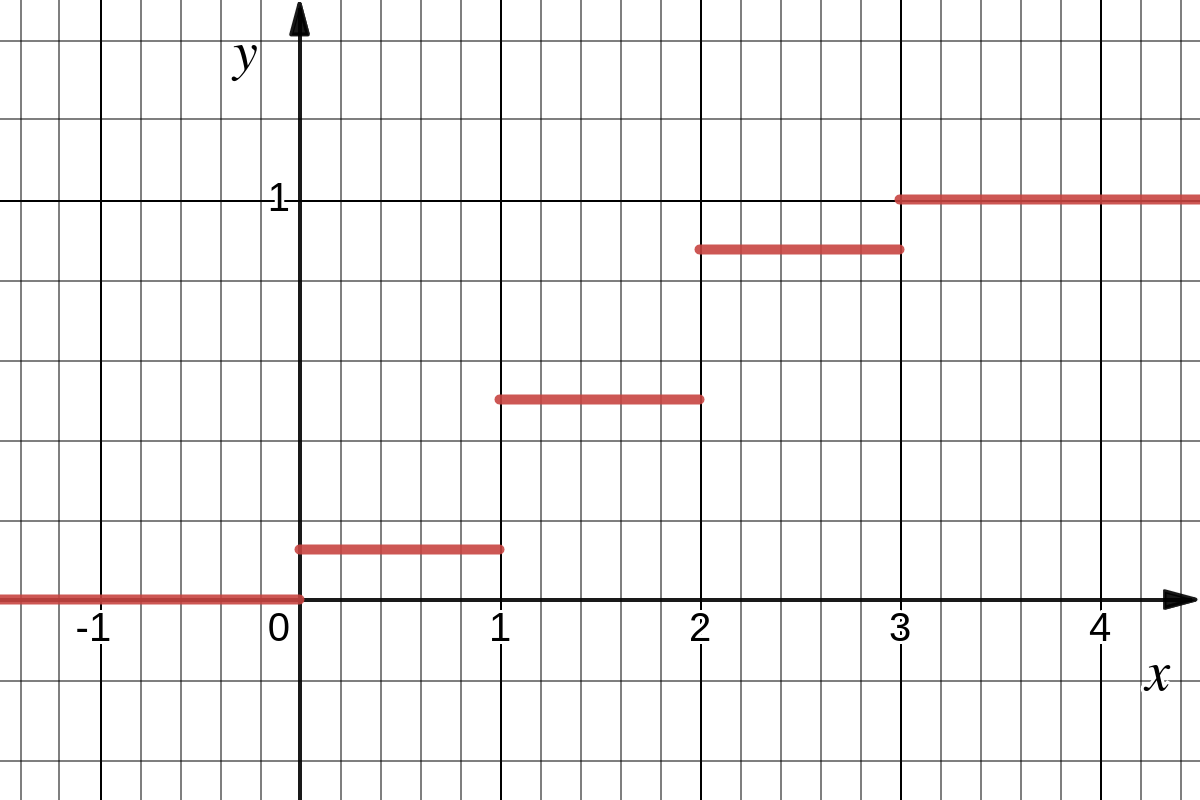
\includegraphics[scale=0.3]{distributionFunction-Example.png}
\caption{Distribution function from Example \ref{Ex:DistributionFunction}}\label{fig:DistributionFromFirstExample}
\end{figure}

\begin{theorem}
Let $X$ be a random variable. Then its distribution function $F_X$ satisfies the following properties:
    \begin{enumerate}[label=\alph*)]
        \item $F_X$ is non-decreasing, meaning $x_1 \leq x_2 \Rightarrow F_X (x_1) \leq F_X (x_2)$;
        \item The set $\{ a < X \leq b \}$ is an event and $P (a < X \leq b ) = F_X (b) - F_X (a)$. 
    \end{enumerate}
\end{theorem}
\begin{proof}
Let $X$ be as in the statement.
    \begin{enumerate}[label=\alph*)]
        \item Assume that $x_1 \leq x_2$. Then, $\{ X \leq x_1 \} \subset \{ X \leq x_2 \}$ and therefore $P (X \leq x_1) \leq P (X \leq x_2 )$. With the notations introduced for the distribution function, this means $F_X (x_1) \leq F_X (x_2)$. 
        \item The set $\{ a < X \leq b \} = \{ X \leq b \} \cap \overline{ \{ X \leq a \}}$. Therefore, it is an event. By the property of the measure $P$, we get
            \[
                P (a < X \leq b) = P (X \leq b) - P (X \leq a ) = F_X (b) - F_X (a) . \qedhere
            \]
    \end{enumerate}
\end{proof}

\section{Continuous Random Variable}

\begin{definition}
A random variable $X$ is \underline{continuous} if its distribution function $F_X$ may be written in the form
\[
    F_X (x) = \int_{-\infty}^x f_X (u) \, du \quad (x \in \mR ) ,
\]
for a map $f_X : \mR \ra [0, \infty )$.  
\end{definition}

\underline{\textbf{Note:}} 
    \begin{itemize}
    \item The function $f_X$ is called the \underline{probability density function} (pdf for short) of $X$. 
    \item It is customary to give the pdf of a continuous random variable instead of the distribution function.
    \item $f_X(x)$ does not represent a probability and its values may even exceed $1$.
    \item In fact, $f_X (x)$ is a measure of probability in the following sense. If $\Delta x$ is small and positive, then the probability that $X$ is near $x$ is
        \begin{align*}
        P (x \leq X \leq x + \Delta x ) = F (x + \Delta x) - F(x) = \int_{x}^{x + \Delta x} f_X (u) \, du \approx f_X (x) \Delta x .
        \end{align*}
    Therefore, the true analogy is between $f_X (x) \Delta x$ and $p_X (x)$, for small $\Delta x$.  
    \item Also, a technical detail that we won't get into is the following. To make sense of the above integral, the function $f$ should be integrable. There is different ways of making sense of the notion of integrability. We will assume we are dealing with Rieman integration.
    \end{itemize}

\begin{theorem}
If $X$ is a continuous random variable with density function $f_X$, then
    \begin{enumerate}[label=\alph*)]
        \item $P (X  = x) = 0$, $\forall x \in \mR$;
        \item $P (a < X \leq b) = \displaystyle \int_a^b f_X (x) \, dx$, for any $a, b \in \mR$ with $a \leq b$.
        \item $\displaystyle\int_{-\infty}^\infty f_X (x) \, dx = 1$. 
    \end{enumerate}
\end{theorem}
\begin{proof}
Let $X$ be as in the Theorem. Therefore, $F_X (x) = \displaystyle \int_{-\infty}^x f_X (u) \, du$.
    \begin{enumerate}[label=\alph*)]
        \item Let $x \in \mR$. For each positive integer $n$, set $A_n := \{ x - 1/n < X \leq x \}$. Then, we see that the sequence $\overline{A}_n$ forms an increasing sequence of events. By the continuity of the probability measure $P$, we have
        \[
            P \Big( \bigcup_{n = 1}^\infty \overline{A}_n \Big) = \lim_{n \ra \infty} P (\overline{A}_n )
        \]
        which implies, using de Morgan's laws and the fact that $P (\overline{A}) = 1 - P (A)$,
        \[
            1 - P \Big( \bigcap_{n = 1}^\infty A_n \Big) = 1 - \lim_{n \ra \infty} P (A_n ) .
        \]
        Therefore,
            \[
                P \Big( \bigcap_{n = 1}^\infty A_n \Big) = \lim_{n \ra \infty} P (X \leq x ) - P (X \leq x - 1/n ) .
            \]
        Since $\lim_{n \ra \infty} x - 1/n = x$, we see that $\bigcap_{n = 1}^\infty A_n = \{ X = x \}$. Hence
            \[
                P (X = x) = \lim_{n \ra \infty} \Big( F_X (x) - F_X (x - 1/n ) \Big) = \lim_{n \ra \infty} \int_{x - 1/n}^x f_X (u) \, du = 0 .
            \]
        \item Since $P (X = a ) = 0$, we have 
            \[
                P (a \leq X \leq b) = P (X = a) + P (a < X \leq b ) = P (a < X \leq b ) .
            \]
        Therefore,
            \[
                P (a < X \leq b) = F_X (b) - F_X (a) = \int_a^b f_X (x) \, dx .
            \]
        \item We have
            \[
                \int_{-\infty}^\infty f_X (x ) \, dx = \lim_{x \ra \infty} \int_{-\infty}^x f_X (u) \, du = \lim_{x \ra \infty} F_X (x) .
            \]
        By the continuity of the probability measure $P$, for any sequence $x_n \ra \infty$, the sets $\{ X \leq x_n \}$ is an increasing sequence with $\bigcup_{n= 1}^\infty \{ X \leq x_n \} = S$ and hence 
            \[
                \lim_{x_n \ra \infty} P (X \leq x_n ) = P \Big( {\bigcup}_{n=1}^\infty \{ X \leq x_n \} \Big) = P (S) = 1 .
            \]
        Therefore, since this is true for any sequence converging to $\infty$:
            \[
                \int_{-\infty}^\infty f_X (x) \, dx = \lim_{x \ra \infty} F_X (x) = \lim_{x \ra \infty} P (X \leq x) = 1 . \qedhere
            \]
    \end{enumerate}
\end{proof}

\begin{example}
A random variable $X$ has density function
    \begin{align*}
    f (x) = \left\{ \begin{matrix} 2x & \text{ if } 0 < x < 1 \\ 0 & \text{ otherwise.} \end{matrix} \right.
    \end{align*}
    \begin{enumerate}[label=\alph*)]
        \item Find the distribution function $F_X$ of $X$.
        \item Find $P (0.25 \leq X \leq 0.75)$.
    \end{enumerate}
\end{example}
\begin{sol*}
    \begin{enumerate}[label=\alph*)]
        \item When $x \leq 0$, then $F_X (x) = 0$. For $0 < x < 1$, we then have
        \[
            F_X (x) = \int_{-\infty}^x f_X (u) \, du = \int_0^x 2u \, du = x^2 .
        \]
        When $x \geq 1$, then
        \[
            F_X (x) = \int_{-\infty}^x f_X (u) \, du = \int_0^1 2u \, du = 1 .
        \]
        \item Using the expression of $F_X$, we have
        \[
            P (0.25 \leq X \leq 0.75 ) = F_X (0.75) - F_X (0.25) = \frac{9}{16} - \frac{1}{16} = \frac{1}{2} . \tag*{$\triangle$}
        \]
    \end{enumerate}
\end{sol*}

\section{Uniform Distribution}

A random variable $X$ is said to have an \underline{uniform distribution} with parameters $a$ and $b$, with $a < b$ if its density function is given by
    \begin{align*}
    f_X (x) = \left\{ \begin{matrix} 1/(b-a) & \text{ if } a < x < b \\ 0 & \text{otherwise.} \end{matrix} \right. 
    \end{align*}
We usually write $X \sim U (a, b)$.

The distribution function $F_X$ is then
    \begin{align*}
    F_X (x) = \int_{-\infty}^x f_X (u) \, du = \left\{ \begin{matrix} 0 & \text{if } x \leq a \\ \frac{x - a}{b - a} & \text{if } a < x < b \\ 1 & \text{if } b \leq x \end{matrix} \right. 
    \end{align*}

Some phenomena in physical, management, and biological sciences can be modeled on a uniform distribution. The assumption are usually that the process follows a Poisson distribution and we know one occurrence has happened within a time interval $(0, t)$.

\begin{example}
Arrivals of customers at a checkout counter follow a Poisson distribution. It is known that, during a given $30$-minute period, one customer arrives at the counter. Find the probability that a customer arrives during the last $5$ minutes of the $30$-minute period.
\end{example}

\begin{sol*}
We assume that it is equally likely that a person arrives at any given minute within the $30$-min period. If $X$ is the minute when a customer shows up, then we assume that $X \sim U (0, 30)$. Therefore,
    \[
        f_X (x) = \frac{1}{30 - 0} \quad (0 \leq x \leq 30 ) .
    \]
We then have
    \[
        P (25 \leq X \leq 30) = \int_{25}^{30} f_X (x) \, dx = \frac{30 - 25}{30} = \frac{1}{6} . \tag*{$\triangle$}
    \]
\end{sol*}

\begin{example}
A parachutist lands at a random point on a line between markers $A$ and $B$. 
    \begin{enumerate}[label=\alph*)]
    \item Find the probability that she is closer to $A$ than to $B$.
    \item Find the probability that her distance to $A$ is more than three times her distance to $B$.
    \end{enumerate}
\end{example}

\begin{sol*}
\begin{enumerate}[label=\alph*)]
\item We assume that any given position between $A$ and $B$ is equally likely to occur, so that if $X$ is the location between $A$ and $B$, then $X \sim U (0, 1)$, where $0 = A$ and $1= B$. 

For her to be closer to $A$, this means that $X < 1/2$. Therefore, the probability is
    \[
        P (X < 1/2) = P (X \leq 1/2) = \int_0^{1/2} \, dx = 1/2 .
    \]
\item Let $x$ be the distance of the parachutist to the point $A$. Then the distance of the parachutist to $B$ is $1 - x$. We want to find when $x \geq 3 (1 - x)$, which is equivalent to 
    \[
        4x \geq 3 \iff x \geq \frac{3}{4} .
    \]
Therefore, the probability is
    \[
        P (X \geq 3/4 ) = 1 - P (X < 3/4) = 1 - 3/4 = \frac{1}{4} . \tag*{$\triangle$}
    \]
\end{enumerate}
\end{sol*}

\section{Functions of Random Variables}

\begin{example}
Let $X$ be a continuous random variable and let $g (x) = 2x + 3$. Find the distribution function of $Y = g(X)$ and its density function $f_Y$.
\end{example}

\begin{sol*}
By definition, $F_Y (y) = P (Y \leq y )$. Since $Y = g(X)$, we have
    \[
        \{ Y \leq y \} = \{ 2X + 3 \leq y \} = \{ X \leq (1/2) (y - 3) \}
    \]
and hence
    \[
        F_Y (y) = P (X \leq (1/2) (y - 3) ) = F_X ( (1/2) (y - 3) ) .
    \]
Therefore, $Y$ is a continuous random variable and
    \[
        f_Y (y) = \frac{d}{dy} \Big( F_X ( (1/2) (y - 3) ) \Big) = f_X \Big( \frac{y - 3}{2} \Big) \frac{d}{dy} \Big( \frac{y - 3}{2} \Big) = f_X \Big( \frac{y - 3}{2} \Big) \Big( \frac{1}{2} \Big) .
    \]
Using the notation $g^{-1} (y) = \frac{y - 3}{2}$, it is possible to rewrite $f_Y (y)$ as
    \[
        f_Y (y) = f_X (g^{-1} (y)) \frac{d}{dy} [g^{-1} (y)] . \tag*{$\triangle$}
    \]
\end{sol*}

\begin{theorem}
Let $X$ be a continuous random variable with density function $f_X$, and let $g : \mR \ra \mR$ be a strictly increasing and differentiable function. Then $Y = g(X)$ is a continuous random variable with density function
    \[
        f_Y (y) = f_X (g^{-1} (y)) \frac{d}{dy} [g^{-1} (y) ] \quad (y \in \mR )
    \]
where $g^{-1}$ is the inverse function of $g$.
\end{theorem}
\begin{proof}
We first find the distribution function of $Y$. Notice that a result from Calculus II (or Introduction to Real Analysis) implies that the inverse function of $g$, $g^{-1}$, exists and $g^{-1}$ is also increasing. We then have
    \[
         Y \leq y \iff g (X) \leq y \iff X \leq g^{-1} (y) .
     \] 
This implies that
    \[
        F_Y (y) = P (Y \leq y) = P (X \leq g^{-1} (y)) = F_X (g^{-1} (y))
    \]
and differentiating both sides, we get
    \[
        f_Y (y) = f_X (g^{-1} (y)) \frac{d}{dy} [g^{-1} (y)] . \qedhere
    \]
\end{proof}

\underline{\textbf{Notes:}} 
    \begin{itemize}
    \item If $g$ is strictly decreasing and differentiable, then the density function $f_Y$ is
        \[
            f_Y (y) = -f_X (g^{-1} (y)) \frac{d}{dy} [g^{-1} (y) ] \quad (y \in \mR ) .
        \]
    \item In the cases where the above result does not apply, we have to treat each case on their own.
    \end{itemize}

\begin{example}
Let $X$ be a continuous random variable. If $Y = X^2$, find the distribution function of $Y$ and its density function.
\end{example}

\begin{sol*}
For $y \leq 0$, we have $F_Y (y) = P (Y \leq y) = 0$, because $Y$ takes only positive values. Assume that $y > 0$. Then,
    \[
        P (Y \leq y ) = P (X^2 \leq y) = P (|X| \leq \sqrt{y}) = P (-\sqrt{y} \leq X \leq \sqrt{y}) 
    \]
and from the properties of the distribution function, we have
    \[
        F_Y (y) = F_X (\sqrt{y}) - F_Y (-\sqrt{y}) .
    \]
Then, differentiating with respect to $y$ gives
    \[
        f_Y (y) = f_X (\sqrt{y}) \frac{1}{2\sqrt{y}} + f_X (-\sqrt{y}) \frac{1}{2 \sqrt{y}} = \frac{f_X (\sqrt{y}) + f_X (-\sqrt{y})}{2 \sqrt{y}} . \tag*{$\triangle$}
    \]
\end{sol*}

\section{Expectations of Continuous Random Variables}

\begin{definition}
If $X$ is a continuous random variable with density $f_X$, then the \underline{expectation} of $X$ is denoted by $\mathrm{Exp} (X)$ and is defined by
    \[
        \mathrm{Exp} (X) = \int_{-\infty}^\infty x f_X (x) \, dx ,
    \]
whenever this integral converges absolutely, meaning that $\displaystyle \int_{-\infty}^\infty |x f_X (x)| \, dx < \infty$. 
\end{definition}

\begin{example}
Find the expectation of a continuous random variable $X \sim U (-1, 1)$. 
\end{example}

\begin{sol*}
By definition, we have
    \[
        \mathrm{Exp} (X) = \int_{-1}^1 x \frac{1}{1 - (-1)} \, dx = \frac{1}{2} (1^2 - (-1)^2)/2 = 0 . \tag*{$\triangle$} 
    \]
\end{sol*}

To be able to derive a useful formula for the variance of a random variable $X$, we need the following result.

\begin{theorem}\label{Thm:LawSubStatis}
If $X$ is a continuous random variable with density $f_X$ and if $g : \mR \ra [0, \infty )$ is a map such that $Y = g(X)$ is a continuous random variable. Then,
    \[
        \mathrm{Exp} (Y) = \int_{-\infty}^\infty g (x) f_X (x) \, dx ,
    \]
whenever this integral converges absolutely.
\end{theorem}

To prove this result, we need the following interesting result.

\begin{lemma}\label{Lem:ExpInTermsOfDistributionFunc}
If $X$ is a continuous random variable taking only non-negative values, then
    \[
        \mathrm{Exp} (X) = \int_0^\infty (1 - F_X (x)) \, dx .
    \]
\end{lemma}
\begin{proof}
By definition of the expectation, 
    \[
        \mathrm{Exp} (X) = \int_{-\infty}^\infty x f_X (x) \, dx .
    \]
Since $X$ takes only positive values, we have that $F_X (x) = 0$ for any $x \leq 0$. Therefore, $f_X (x) = 0$ for any $x \leq 0$ and
    \[
        \mathrm{Exp} (X) = \int_0^\infty x f_X (x) \, dx .
    \]
Using the fact that $x = \displaystyle\int_0^x  \, dt$, we have
    \[
        \mathrm{Exp} (X) = \int_0^\infty \int_0^t f_X (x) \, dt dx .
    \]
From Fubini's Theorem, we get
    \[
        \mathrm{Exp} (X) = \int_0^\infty \int_t^\infty f_X (x) \, dx dt = \int_0^\infty \Big( 1 - 1 + \int_t^\infty f_X (x) \, dx \Big) \,  dt .
    \]
Using the fact that $1 = \int_{0}^{\infty} f_X (x) \, dx$, we find that
    \[
        1 - 1 + \int_t^\infty f_X (x) \, dx = 1 - \int_0^\infty f_X (x) \, dx + \int_t^\infty f_X (x) \, dx = 1 - \int_0^t f_X (x) \, dx = 1 - F_X (t) .
    \]
Hence,
    \[
        \mathrm{Exp} (X) = \int_0^\infty (1 - F_X (t)) \, dt . \qedhere
    \]

\end{proof}

\begin{proof}[Proof of Theorem \ref{Thm:LawSubStatis}]
Since $g$ takes only non-negative values, the continuous random variable $Y = g(X)$ takes only non-negative values. Lemma \ref{Lem:ExpInTermsOfDistributionFunc} then implies
    \[
        \mathrm{Exp} (Y) = \int_0^\infty (1 - F_Y (u) ) \, du = \int_0^\infty 1 - P (g(X) \leq u ) \, du .
    \]
Recall that $P (Y < \infty ) = \int_{-\infty}^\infty f_Y (t) \, dt = 1$, so that
    \[
        \mathrm{Exp} (Y) = \int_0^\infty P (g(X) > u ) \, du = \int_0^\infty \Big( \int_B f_X (x) \, dx \Big) du ,
    \]
where $B = \{ x \, : \, g(x) > u \}$. Using Fubini's Theorem, we get
    \[
        \mathrm{Exp} (Y) = \int_0^\infty \int_0^{g(x)} \, du \, f_X (x) \, dx = \int_0^\infty g(x) f_X (x) \, dx . \qedhere
    \]
\end{proof}

\underline{\textbf{Note:}} Theorem \ref{Thm:LawSubStatis} remains true if we have a function $g : \mR \ra \mR$. In this case, we have to write $g = g_+ - g_-$, where $g_+$ and $g_-$ are defined as followed:
    \[
        g_+ (x) = \max \{ g (x) , 0 \} \quad \text{ and } \quad g_- (x) = \max \{ -g(x) , 0 \} 
    \]
and apply Lemma \ref{Lem:ExpInTermsOfDistributionFunc} to $g_+$ and $g_-$.

As we did in the discrete case, we define the variance as the expectation of $(X - \mathrm{Exp} (X))^2$.

\begin{definition}
Let $X$ be a continuous random variable, then the \underline{variance} of $X$ is denoted by $\mathrm{Var} (X)$ and is defined by
    \[
        \mathrm{Var} (X) = \mathrm{Exp} ( (X - \mu )^2 ) ,
    \]
where $\mu := \mathrm{Exp} (X)$. 
\end{definition}

Using Theorem \ref{Thm:LawSubStatis} with $g (x) = (x - \mu)^2$, we find that
    \[
        \mathrm{Var} (X) = \int_{-\infty}^\infty (x - \mu )^2 f_X (x) \, dx = \mathrm{Exp} (X^2) - \mu^2 .
    \]

\begin{example}
Find the variance of $X \sim U (a, b)$. 
\end{example}

\begin{sol*}
From the above formula, we have $\mathrm{Var} (X) = \mathrm{Exp} (X^2 ) - \mu^2$, where $\mu = \mathrm{Exp} (X)$. We have
    \[
        \mathrm{Exp} (X) = \int_{-\infty}^\infty xf_X (x) \, dx = \int_a^b \frac{x}{b-a} \, dx = \frac{a + b}{2} ,
    \]
and
    \[
        \mathrm{Exp} (X^2) = \int_{-\infty}^\infty x^2 f_X (x) \, dx = \int_a^b \frac{x^2}{b- a} \, dx = \frac{a^2 + ab + b^2}{3} .
    \]
Hence
    \[
        \mathrm{Var} (X) = \frac{a^2 + ab + b^2}{3} - \frac{a^2 + 2ab + b^2}{4} = \frac{(b - a)^2}{12} . \tag*{$\triangle$} 
    \]
\end{sol*}

\section{Other Examples of Continuous Random Variables}

\subsection*{Normal Distribution}

A random variable $X$ is said to have a \underline{normal distribution} with parameters $\mu$ and $\sigma$ if its density function is given by
    \begin{align*}
    f_X (x) = \frac{1}{\sqrt{2\pi \sigma^2}} \exp \Big( -\frac{1}{2 \sigma^2} (x - \mu )^2 \Big) .
    \end{align*}
We usually write $X \sim N (\mu , \sigma )$. We have $\mathrm{Exp} (X) = \mu$ and $\mathrm{Var} (X) = \sigma^2$. 

The distribution function $F_X$ can not be given in a closed form. We usually use a table that contains approximations of the value of $F_X$. 

The normal distribution is one of the most important distribution out there. We will see later that a lot of phenomena can be approximated by a normal distribution. We first need the following result.

\begin{theorem}\label{Thm:StandardNormalDistribution}
Let $X \sim N (\mu , \sigma )$ be a continuous random variable and let $Z = (X - \mu )/ \sigma$. Then $Z \sim N (0, 1)$.
\end{theorem}
\begin{proof}
With $g(x) = (x - \mu ) / \sigma$ so that $g^{-1} (z) = \sigma z + \mu$. Therefore, the density function of $Z$ is
    \[
        f_Z (z) = f_X (\sigma z + \mu ) \sigma = \frac{\sigma}{\sqrt{2\pi\sigma^2}} \exp \Big(-\frac{1}{2\sigma^2} (\sigma z + \mu - \mu )^2 \Big) = \frac{1}{\sqrt{2\pi}} \exp \Big( -\frac{z^2}{2} \Big) . \qedhere
    \]
\end{proof}

\begin{example}
The achievement scores of college entrance examination are normally distributed with mean 75 and standard deviation $10$. What fraction of the scores lies between $80$ and $90$?
\end{example}

\begin{sol*}
We have $\mu = 75$ and $\sigma = 10$. We create the new random variable $Z = (X - \mu)/ \sigma$, so that $Z \sim N (0, 1)$ from Theorem \ref{Thm:StandardNormalDistribution}. Therefore,
    \[
        80 \leq X \leq 90 \iff \frac{80-75}{\sigma} \leq Z \leq \frac{90 - 75}{10} \iff 0.5 \leq Z \leq 1.5 .
    \]
The probability we are looking for is $P (80 \leq X \leq 90 ) = P (0.5 \leq Z \leq 1.5 )$. Using the table, we have
    \[
        P (0.5 \leq Z \leq 1.5) = 0.93319 - 0.69146 = 0.24173 . \tag*{$\triangle$}
    \]
\end{sol*}

\subsection*{Exponential Distribution}

A random variable $X$ is said to have an \underline{exponential distribution} with parameter $\lambda > 0$ if its density function is given by
    \begin{align*}
    f_X (x) = \left\{ \begin{matrix} \lambda e^{-\lambda x} & \text{if } x > 0 \\ 0 & \text{if } x \leq 0 \end{matrix} \right. 
    \end{align*}
We usually write $X \sim \mathrm{Poisson} (\lambda )$. We have $\mathrm{Exp} (X) = 1/\lambda$ and $\mathrm{Var} (X) = 1/\lambda^2$.

The distribution function $F_X$ is then
    \begin{align*}
    F_X (x) = \left\{ \begin{matrix} 0 & \text{if } x \leq 0 \\ 1 - e^{-\lambda x} & \text{if } x > 0. \end{matrix} \right. 
    \end{align*}

\subsection*{Beta Distribution}

A random variable $X$ is said to have a \underline{beta distribution} with parameters $\alpha , \beta > 0$ if the density function $X$ is
    \[
        f_X (x) = \left\{ \begin{matrix} \displaystyle \frac{x^{\alpha - 1} (1 - x)^{\beta - 1}}{B (\alpha , \beta )} & \text{, } 0 \leq x \leq 1 \\ 
        0 & \text{elsewhere,} \end{matrix} \right. 
    \]
where
    \[
        B(\alpha , \beta ) = \int_0^1 t^{\alpha - 1} (1 - t)^{\beta - 1} \, dt = \frac{\Gamma (\alpha ) \Gamma (\beta )}{\Gamma (\alpha + \beta ) } .
    \]
We have $\mathrm{Exp} (X) = \alpha / (\alpha + \beta )$ and $\mathrm{Var} (X) = \frac{\alpha \beta}{(\alpha + \beta)^2 (\alpha + \beta + 1)}$.


\begin{comment}

\section{Problems Set}

\subsection*{Distribution Function}

\begin{problem}
Let $F_1$ and $F_2$ be two distribution functions. Show that the function $F(x) = \alpha F_1 (x) + (1 - \alpha ) F_2 (x)$ is a distribution function, for any $\alpha$ satisfying $0 \leq \alpha \leq 1$.
\end{problem}

\begin{problem}
Given a random variable $X$, express the distribution function of $Y = \max \{ 0, X \}$ is terms of the distribution function of $X$.
\end{problem}

\begin{problem}
For which value of $c$ is the function
    \[
        F(x) = c\int_{-\infty}^x e^{-|t|} \, dt \quad (x \in \mR )
    \]
a distribution function?
\end{problem}

\subsection*{Continuous Random Variable}

\begin{problem}
Assume that a continuous random variable $X$ has distribution function
    \[
        F(x) = \left\{ \begin{matrix} \displaystyle \frac{1}{2 (1 + x^2)} & -\infty < x \leq 0 \\
        \displaystyle \frac{1 + 2x^2}{2 (1 + x^2)} & 0 < x < \infty \end{matrix} \right.
    \]
Find the density function of $X$. 
\end{problem}

\begin{problem}\label{Prob:FindDistroFunction}
Let the density function of a random variable $X$ be given by
    \[
        f_X (x) = \left\{ \begin{matrix} \displaystyle \frac{2}{\pi (1 + x^2 )} & -1 \leq x \leq 1 \\
        0 & \text{elsewhere.} \end{matrix} \right. 
    \]
Find the distribution function of $f_X$. 
\end{problem}

\begin{problem}\label{Prob:FindDistroFunction2}
A random variable $X$ has density function
    \[
        f_X (x) = c x (x - 1) \quad (0 \leq x \leq 1 ) 
    \]
and $0$ elsewhere. Determine $c$ so that $F_X$ is a distribution function.
\end{problem}

\subsection*{Functions of Random Variables}

\begin{problem}
Let $X$ be a random variable with the exponential distribution with parameter $\lambda$. Find the density function of
    \begin{enumerate}[label=\alph*)]
        \item $Y = 2X + 5$.
        \item $Y = (1 + X)^{-1}$.
    \end{enumerate}
\end{problem}

\begin{problem}
Let $X$ be a random variable whose distribution function $F$ is a continuous function. Show that the random variable $Y$, defined by $Y = F(X)$, is uniformly distributed on the interval $(0, 1)$.
\end{problem}

\begin{problem}
The random variable $X$ is uniformly distributed on the interval $[0, 1]$. Find the distribution and probability density function $Y$, where
    \[
        Y = \frac{3X}{1 - X} .
    \]
\end{problem}

\subsection*{Expectation of Continuous Random Variables}

\begin{problem}
Find the expectation of the random variable $X$ given in Problem \ref{Prob:FindDistroFunction}.
\end{problem}

\begin{problem}
Find the expectation and variance of $X$ given in Problem \ref{Prob:FindDistroFunction2}.
\end{problem}

\subsection*{Other Examples of Continuous Random Variables}

\begin{problem}
If $Z \sim N (0, 1)$ is a random variable that has the standard normal distribution, what is
    \begin{enumerate}[label=\alph*)]
        \item $P (Z^2 < 1 )$?
        \item $P (Z^2 < 3.84146)$?
    \end{enumerate}
\end{problem}

\begin{problem}
A soft-drink machine can be regulated so that it discharges an average of $\mu$ ounces per cup. If the ounces of fill are normally distributed with stardard deviation $0.3$ ounce, give the setting for $\mu$ so that $8$-ounce cups will overflow only $1\%$ of the time.
\end{problem}

\begin{problem}
Prove that
    \[
        \int_{-\infty}^\infty e^{-x^2} \, dx = \sqrt{\pi} .
    \]
\end{problem}

\begin{problem}
If $X$ has the normal distribution with mean $0$ and variance $1$, find the mean value of $Y = e^{2X}$.
\end{problem}

\begin{problem}
Suppose that $X$ has an exponential distribution with parameter $\lambda$. Show that, if $a > 0$ and $b > 0$, then
    \[
        P (X > a + b | X > a) = P (X > b) .
    \]
\end{problem}


\section{Solutions to Problems Set}
\setcounter{problem}{0} 

\subsection*{Distribution Function}

\begin{problem}

Let $\alpha$ be a number between $0$ and $1$. If $x_1 \leq x_2$, then
    \[
        F(x_1) = \alpha F_1(x_1) + (1 - \alpha ) F_2 (x_2) \leq \alpha F_1 (x_2) + (1 - \alpha ) F_2 (x) = F (x_2) .
    \]
Therefore, $F$ is inscreasing. We also have
    \[
        \lim_{x \ra \infty} F(x) = \lim_{x \ra \infty} \alpha F_1 (x) + (1 - \alpha ) F_2 (x) = \alpha \lim_{x \ra \infty} F_1 (x) + (1 - \alpha ) \lim_{x \ra \infty} F_2 (x) = \alpha (1) + (1 - \alpha ) (1) = 1 .
    \]
Therefore, $F$ is distribution function. \hfill $\square$
\end{problem}

\begin{problem}
The values of $Y$ are always positive, so if $y < 0$, then $F_Y(y) = 0$. If $y \geq 0$, then $Y = X$ and therefore $F_Y (y) = F_X (y)$. Therefore, $F_Y = \max \{ 0 , F_X \}$. 
\end{problem}

\begin{problem}
The total integral should be $1$. We have
    \[
        \int_{-\infty}^\infty e^{-|t|} \, dt = 2
    \]
so that
    \[
        2c = 1 \quad \Rightarrow \quad c = 1/2 . \tag*{$\square$}
    \]
\end{problem}

\subsection*{Continuous Random Variable}

\begin{problem}
For $x < 0$, we can differentiate and get
    \[
        f_X (x) = \frac{d}{dx} F_X (x) = \frac{d}{dx} \Big( \frac{1}{2 (1 + x^2 ) }\Big) = \frac{-x}{(1 + x^2)^2} .
    \]
For $x > 0$, we can differentiate and get
    \[
        f_X (x) = \frac{d}{dx} F_X (x) = \frac{d}{dx} \Big( \frac{1 + 2x^2}{2 (1 + x^2)} \Big) = \frac{x}{(1 + x^2)^2} .
    \]
At $x = 0$, $f_X(0)$ is not defined. \hfill $\square$
\end{problem}

\begin{problem}\label{Prob:FindDistroFunction}
When $x < -1$, then $F_X (x) = 0$ because $f_X (x) = 0$. When $-1 \leq x < 1$, then
    \[
        F_X (x) = \int_{-1}^x \frac{2}{\pi (1 + t^2)} \, dt = \frac{2}{\pi} \arctan (x) + 1/2
    \]
When $x \geq 1$, then
    \[
        F_X (x) = \frac{2}{\pi} \arctan (1) + \frac{1}{2} = 1 .
    \]
Hence
    \[
        F_X (x) = \left\lbrace \begin{matrix} 0 & x < -1 \\ 
        \frac{2}{\pi} \arctan (x) + \frac{1}{2} & -1 \leq x \leq 1 \\ 
        1 & x > 1 . \end{matrix} \right. \tag*{$\square$}
    \]
\end{problem}

\begin{problem}\label{Prob:FindDistroFunction2}
We must have $\lim_{x \ra \infty} F_X (x) = 1$, and so
    \[
        c\int_0^1 x (x - 1) \, dx = 1 \iff -\frac{c}{6} = 1 .
    \]
Hence we must have $c = -6$. \hfill $\square$
\end{problem}

\subsection*{Functions of Random Variables}

\begin{problem}
When $Y = g (X)$ and $g$ is increasing, then we use the formula
    \[
        f_Y (y) = f_X (g^{-1} (y)) \frac{d}{dy} (g^{-1} (y)) .
    \]
Since $X$ has the exponential distribution,
    \[
        f_Y (y) = \lambda e^{-\lambda g^{-1} (y)} \frac{d}{dy} (g^{-1} (y)) .
    \]
When $g$ is decreasing, then
    \[
        f_Y (y) = - \lambda e^{-\lambda g^{-1} (y)} \frac{d}{dy} (g^{-1} (y)) .
    \]

    \begin{enumerate}[label=\alph*)]
        \item We have $g^{-1} (y) = (y - 5)/2$. Since $g$ is increasing, with $\frac{d}{dy} (g^{-1} (y)) = 1/2$, we obtain
            \[
                f_Y (y) = \frac{\lambda}{2} e^{-\frac{\lambda}{2} (y - 5)} .
            \]
        \item The inverse is found in the following way. Set $y = (1 + x)^{-1}$ and then
            \[
                y (1 + x) = 1 \iff y + yx = 1 \iff x = \frac{1 - y}{y} .
            \]
        Therefore $g^{-1} (y) = (1 - y)/y$. Since $g$ is decreasing, with $\frac{d}{dy} (g^{-1} (y)) = -1/(1-y)^2$, we obtain
            \[
                f_Y (y) = \frac{\lambda e^{-\frac{\lambda (1 - y)}{y}} (1 - y)}{y}. \tag*{$\square$}
            \]
    \end{enumerate}
\end{problem}

\begin{problem}
Since the range of $F$ is between $0$ and $1$, then $\im Y \in [0, 1]$ with each number between $0$ and $1$ being attained because of the continuity of $F$.

Since $F$ is an increasing function, we can apply the formula to find the density function of $Y$. For $y \in [0, 1]$, we have
    \[
        f_Y (y) = f_X (F^{-1} (y)) \frac{d}{dy} (F^{-1} (y)) .
    \]
Since $X$ is a continuous random variable, we have 
    \[
        F(x) = \int_{-\infty}^x f_X (t) \, dt .
    \]
A formula for the derivative of the inverse in terms of the initial function $F$ is
    \[
        \frac{d}{dy} (F^{-1} (y)) = \frac{1}{F' (F^{-1} (y))} .
    \]
Since $F' (x) = f_X (x)$, we therefore obtain
    \[
        f_Y (y) = \frac{f_X (F^{-1} (y))}{f_X (F^{-1} (y))} = 1 .
    \]
Therefore, the density function of $Y$ is $1$ identically on $[0, 1]$. Thus, $Y$ has a uniform distribution on $[0, 1]$. \hfill $\square$
\end{problem}

\begin{problem}
Set $g (x) = \frac{3x}{1 - x}$. Then, $g' (x) = \frac{1}{(1 - x)^2}$. The derivative is always positive, so $g$ is increasing. The density function of $Y$ is then given by the following formula:
    \[
        f_Y (y) = f_X (g^{-1} (y)) \frac{d}{dy} (g^{-1} (y)) .
    \]
After some calculations, we obtain
    \[
        g^{-1} (y) = \frac{y}{y + 3} \quad \text{ and } \quad \frac{d}{dy} (g^{-1} (y)) = \frac{3}{(3 + y)^2} .
    \]
Hence,
    \[
        f_Y (y) = f_X \Big( \frac{y}{y + 3} \Big) \frac{3}{(3 + y)^2} .
    \]
When $-3 < y < 0$, then $\frac{y}{y + 3} < 0$ because $y + 3 > 0$. Therefore $f_X (y/(y + 3)) = 0$. 

If $y \geq 0$, then $0 \leq \frac{y}{y + 3} \leq 1$, because $y \leq y + 3$ and $y + 3$ is positive. Therefore, $f_X (y/(y +3)) = 1$ and then
    \[
        f_Y (y) = \frac{3}{(3 + y)^2} ,
     \]
when $y \geq 0$.

If $y < -3$, then $y < y + 3$ implies that $1 > \frac{y + 3}{y}$ and therefore $\frac{y}{y + 3} > 1$. Therefore, $f_Y (y) = 0$. 

Hence, we get
    \[
        f_Y (y) = \left\lbrace \begin{matrix} 0 & y < 0 \\ 
        \frac{3}{(3 + y)^2} & y \geq 0 .
        \end{matrix} \right.
    \]

We can now find the distribution of $Y$. When $y < 0$, $F_Y (y)= 0$ because $f_Y (y) = 0$. When $y \geq 0$, then
    \[
        F_Y (y) = \int_0^y \frac{3}{(3 + t)^2} \, dt = \left. \Big( \frac{-3}{3 + t} \Big) \right|_0^y = 1 - \frac{3}{3 + y} .
    \]
Notice that $F_Y (y) = \frac{y}{y + 3} = g^{-1} (y)$, when $y \geq 0$. \hfill $\square$
\end{problem}

\subsection*{Expectation of Continuous Random Variables}

\begin{problem}
The expectation is
    \begin{align*}
        \mathrm{Exp} (X) &= \int_{-\infty}^\infty x f_X (x) \, dx \\ 
        &= \int_{-1}^1 \frac{2x}{\pi (1 + x^2 )} \, dx \\ 
        &= 0
    \end{align*}
because the function $\frac{2x}{\pi (1 + x^2 )}$ is an odd function. The expected value of $X$ is therefore $0$. \hfill $\square$ 
\end{problem}

\begin{problem}
The expectation is
    \[
        \int_{-\infty}^\infty x f_X (x) \, dx = \int_0^1 -6 x^2 (x - 1) \, dx = \frac{1}{2} . 
    \]
The variance is
    \[
        \mathrm{Exp} (X^2) - (\mathrm{Exp} (X))^2 = \int_{-0}^1 -6 x^3 (x -1) \, \ dx - \frac{1}{4} = \frac{3}{10} - \frac{1}{4} = \frac{1}{20} .\tag*{$\square$}
    \]
\end{problem}

\subsection*{Other Examples of Continuous Random Variables}

\begin{problem}
    \begin{enumerate}[label=\alph*)]
        \item We have $Z^2 < 1$ if and only if $-1 < Z < 1$. Therefore, 
            \[
                P (Z^2 < 1) = P (-1 < Z < 1 ) = P (Z < 1) - P (Z \leq -1) = P (Z \leq 1 ) - P (Z \leq -1).
            \]
        Using the table, 
            \[
                P (Z^2 < 1) = 0.84134 - 0.15866 = 0.68268 .
            \]
        \item Similar calculations:
            \[
                P (Z^2 < 3.84146) = P (Z < 1.96) - P (Z < -1.96) = 0.975 - 0.0025 = 0.950 . \tag*{$\square$}
            \]
    \end{enumerate}
\end{problem}

\begin{problem}
Define $Z = \frac{X - \mu}{0.3}$, so that $Z \sim N (0, 1)$. We want to know for which $\mu$, $P (X > 8) = 0.01$. Using $Z$, we want to find $\mu$ such that
    \[
        P \Big( Z > \frac{8 - \mu}{0.3} \Big) = 0.01  \iff P \Big( Z \leq \frac{8 - \mu}{0.3} \Big) = 0.99
    \]
The $z$-score corresponding to a probability of $0.1$ is $z = 2.325$. Therefore
    \[
        \frac{8 - \mu}{0.3} = 2.325 \iff \mu = 7.3025 . \tag*{$\square$}
    \]
\end{problem}

\begin{problem}
This is a little trick from Calculus IV. Let $I$ denote the integral we want to compute. Consider 
    \[
        I^2 = \Big( \int_{-\infty}^\infty e^{-x^2} dx \Big) \Big( \int_{-\infty}^\infty e^{-y^2} \, dy \Big) = \int_{-\infty}^\infty \int_{-\infty}^\infty e^{-x^2 - y^2} \, dy dx .
    \]
Let $R = \{ (x, y) \, : \, -\infty < x < \infty , -\infty < y < \infty \}$. Using polar coordinates, we see that $R = \{ (r, \theta ) \, : \, 0 \leq r < \infty , 0 \leq \theta \leq 2\pi \}$. Therefore,
    \[
        I^2 = \iint_R e^{-x^2 - y^2} \, dA = \int_0^{2\pi} \int_0^\infty r e^{-r^2} \, dr d\theta 
    \]
Using $u = r^2$, we see that
    \[
        \int_0^\infty re^{-r^2} \, dr = \frac{1}{2} \int_0^\infty e^{-u} \, du = \frac{1}{2} 
    \]
and hence
    \[
        I^2 = \pi \quad \Longrightarrow \quad I = \sqrt{\pi} . \tag*{$\square$}
    \]
\end{problem}

\begin{problem}
Here, we have $g (x) = e^{2x}$. Since it is an increasing function with $g^{-1} (y) = \frac{1}{2} \ln y$, using the formula, the density function of $Y$ is
    \[
        f_Y (y) = \frac{e^{-\frac{1}{4} (\ln (y))^2}}{2 \sqrt{2\pi} y} \quad (\text{for } y > 0) .
    \]
Therefore, the expected value is
    \[
        \mathrm{Exp} (Y) = \int_{-\infty}^\infty y f_Y (y) \, dy = \frac{1}{2 \sqrt{2\pi}} \int_0^\infty e^{-( \frac{\ln (y)}{2})^2} \, dy .
    \]
Let $u = \ln (y) / 2$, so that $du = \frac{1}{2y} \, dy$. This means
    \[
        \mathrm{Exp} (Y) = \frac{1}{\sqrt{2\pi}} \int_{-\infty}^\infty e^{-u^2}e^{2u} \, du = \frac{e}{\sqrt{2\pi}} \int_{-\infty}^\infty e^{- (u - 1)^2} \, du = e . \tag*{$\square$}
    \]
\end{problem}

\begin{problem}
If $X$ has the exponential distribution, then
    \[
        F_X (x) = \int_0^x \lambda e^{-\lambda t} \, dt = 1 - e^{-\lambda x} \quad (x > 0 ) .
    \]
Since $a, b > 0$, notice that
    \[
        \{ X > a + b \} \cap \{ X > a \} = \{ X > a + b \} .
    \]
Therefore, by definition of the conditional probability,
    \[
        P (X > a + b | X > a ) = \frac{P (X > a + b)}{P (X > a )} = \frac{1 - (1 - e^{-\lambda (a + b)})}{1 - (1 - e^{-\lambda a})} = e^{-\lambda b} = P (X > b ) . \tag*{$\square$}
    \]
\end{problem}

\end{comment}

%%%%%%%%%%%%%%%%%%%%%%%%%%%%%%%%%%%%%%%%
%%%%%%%%%%%% CHAPTER E %%%%%%%%%%%%%%%%%

\chapter{Random Vectors}

In this chapter, we assume that a probability space $(S, \mathcal{A}, P)$ is given.

\section{Bivariate Distributions}
Given two random variables $X$ and $Y$ defined on the probability space $(S, \mathcal{A} , P )$, we can think of them acting together as a random vector $(X, Y)$ taking values in $\mR^2$. 

\begin{example}
Let $S = \{ \epsdice{1} , \epsdice{2} , \epsdice{3} , \epsdice{4} , \epsdice{5} , \epsdice{6} \}$ with $\mathcal{A} = \mathcal{P} (S)$ be the probability space associated to throwing a fair dice. Assume that we throw two such die and consider the following random variable:
\begin{enumerate}[label=\arabic*)]
    \item $X$: ``The number of dots on the first dice''.
    \item $Y$: ``The number of dots on the second dice''.
\end{enumerate}
Assuming the two dice are independent, what is the probability that $X \leq 2$ and $Y \leq 2$?
\end{example}

\begin{sol*}
Denote this probability by $p$. There is $1/6$ chance of obtaining all the different faces. If $A = \{ X \leq 2 \} \cap \{ Y \leq 2 \}$, then
    \begin{align*}
        p &= P (A) \\ 
        &= P (X = 1, Y = 1) + P (X = 1, Y = 2) + P (X = 2, Y = 1) + P (X = 2, Y = 2) \\ 
        &= \frac{1}{36} + \frac{1}{36} + \frac{1}{36} + \frac{1}{36} \\ 
        &= \frac{4}{36} = \frac{1}{9} .
    \end{align*}
We denote $p$ by $F_{X, Y} (2, 2)$ and this is called the joint distribution function of $X$ and $Y$ at $ (X, Y) = (2, 2)$. \hfill $\triangle$
\end{sol*}

\textbf{Notations:}
    \begin{itemize}
        \item the set $\{ s \, : \, X (s) \leq x , Y (s) \leq y \} = \{ X \leq x \} \cap \{ Y \leq y \}$ will be denoted by $\{ X \leq x , Y \leq y \}$.
        \item the probability of $\{ X \leq x , Y \leq y \}$ is denoted by $P (X \leq x , Y \leq y )$. 
    \end{itemize}

\begin{definition}
The \underline{joint distribution function} of a pair of random variables $X$, $Y$ is the mapping $F_{X, Y} : \mR^2 \ra [0, 1]$ given by
    \[
        F_{X, Y} (x, y) = P (X \leq x , Y \leq y ) .
    \]
\end{definition}

\underline{Basic Properties:}
    \begin{enumerate}[label=\arabic*)]
        \item $\displaystyle \lim_{x \ra -\infty} \lim_{y \ra -\infty} F_{X, Y} (x, y) = \lim_{y \ra -\infty} \lim_{x \ra -\infty} F_{X, Y} (x, y) = 0$.
        \item $\displaystyle\lim_{x \ra \infty} \lim_{y \ra \infty} F_{X, Y} (x, y) = \lim_{y \ra \infty} \lim_{x \ra \infty} F_{X, Y} (x, y) = 1$.
        \item Increasing: $F(x_1, y_1) \leq F(x_2, y_2)$, for any $x_1 \leq x_2$ and $y_1 \leq y_2$.
        \item\label{P:MarginalInX}$F_X (x) = \displaystyle \lim_{y \ra \infty} F_{X, Y} (x, y)$. [Proof: Notice that $\{ Y < \infty \} = S$, so that
        \[
            F_X (x) = P (X \leq x ) = P (X \leq x , Y < \infty ) = \lim_{y \ra \infty} F_{X, Y} (x, y) .]
        \]
        \item\label{P:MarginalInY} $F_Y (y) = \displaystyle \lim_{x \ra \infty} F_{X, Y} (x, y)$.
    \end{enumerate}

\begin{definition}
If $X$ and $Y$ are random variables, then the above limits in items 4 and 5 are called the \underline{marginal distributions} of the random vector $(X, Y)$.
\end{definition}

\begin{example}
Assume that $X$ and $Y$ are random variables with joint distribution function
    \[
        F_{X, Y} = \left\lbrace \begin{matrix} 1 - e^{-x} - e^{-y} + e^{-x-y} & \text{if } x, y \geq 0 .\\
        0 & \text{otherwise.} \end{matrix} \right. 
    \]
Find the marginals of this joint distribution.
\end{example}

\begin{sol*}
We first let $y \ra \infty$, so that, if $x \geq 0$, then 
    \[
        \lim_{y \ra \infty} F_{X, Y} (x, y) = \lim_{y \ra \infty} 1 - e^{-x} - e^{-y} + e^{-x - y} = 1 - e^{-x} .
    \]
When $x < 0$, then $F_{X, Y} (x, y) = 0$. Therefore, this gives us $F_X (x) = \max \{ 0 , 1 - e^{-x} \}$, which is the distribution function of the exponential distribution with parameter $\lambda = 1$. Similarly, $F_Y (y) = \max\{ 0, 1 - e^{-y} \}$. \hfill $\triangle$
\end{sol*}

Notice that, in the last example, 
    \[
        F_{X, Y} (x, y) = F_X (x) F_Y (y)
    \]
meaning that
    \[
        P (X \leq x , Y \leq y) = P (X \leq x) P (Y \leq y) .
    \]
When this happens, we say that $X$ and $Y$ are independent.

\begin{definition}
Let $X$ and $Y$ be two random variables with joint distribution function $F_{X, Y}$. Then $X$ and $Y$ are \underline{independent} if for every $x, y \in \mR$,
    \[
        F_{X, Y} (x, y) = F_X (x) F_Y (y)    \]
where $F_X$ and $F_Y$ are the marginals of $X$ and $Y$ respectively.
\end{definition}

\underline{\textbf{Remark.}} When $X$ and $Y$ are not independent, we say that they are \underline{dependent}.

\section{Continuous Random Vectors}

\begin{definition}
Two random variables $X$, $Y$ are \underline{(jointly) continuous} if there is an integrable function $f : \mR \times \mR \ra [0, \infty )$ such that
    \[
        F_{X, Y} (x, y) = \iint_{R} f(u, v) \, dA \,
    \]
for every $x, y \in \mR$, where $R = (-\infty , x] \times (-\infty , y]$.
\end{definition}

\underline{\textbf{Remark:}} 
    \begin{itemize}
    \item When $X$ and $Y$ are jointly continuous, the function $f(x, y)$ in the integral is usually called the \underline{joint probability density function} and usually denoted by $f_{X, Y}$. 
    \item Recall from multivariable calculus that, in cartesian coordinates,
        \[
            \iint_R f (u, v) \, dA  = \int_{-\infty}^x \int_{-\infty}^y f(u, v) \, dv du .
        \]
    \item What we mean by an integrable function is a function $f : \mR \times \mR \ra [0, \infty )$ such that
        \[
            \int_{-\infty}^\infty \int_{-\infty}^\infty f (x, y) \, dx dy < \infty .
        \]
    \end{itemize}

\begin{example}\label{Ex:JointDensityRadioactiveParticle}
Suppose that a radioactive particle is randomly located in a square with sides of unit length. That is, if two regions within the unit square and of equal area are considered, the particle is equally likely to be in either region. Let $X$ and $Y$ denote the coordinates of the particle's location. A reasonable model for the joint probability density function of $X$ and $Y$ is
    \[
        f_{X, Y} (x, y) = \left\lbrace \begin{matrix} 1 & \text{if } (x, y) \in [0, 1] \times [0, 1] \\
        0 & \text{elsewhere.} \end{matrix} \right.
    \]
\begin{enumerate}[label=\alph*)]
    \item Sketch the probability density function.
    \item Find $F(0.2, 0.4)$.
    \item\label{Ex:PartcOfRadioActiveParticle} Find $P (0.1 \leq X \leq 0.3 , 0 \leq Y \leq 0.5)$.
    \item Find $P (X + Y \leq 0.5 )$.
\end{enumerate}
\end{example}

\begin{sol*}
\begin{enumerate}[label=\alph*)]
\item Using Desmos 3D online app, the joint density function looks like this:
    \begin{figure}[ht]
    \centering 
    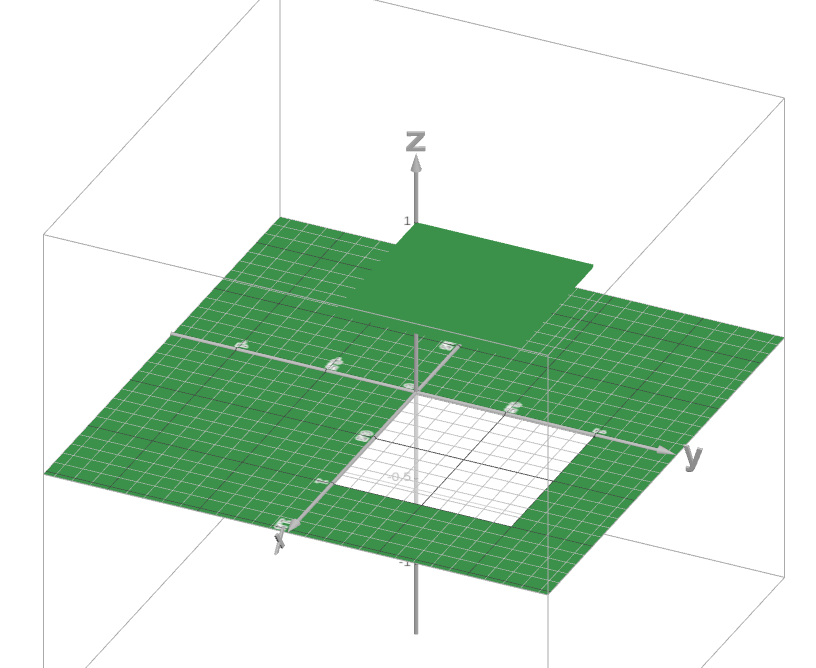
\includegraphics[scale=0.2]{JointDistributionChapE.png}
    \end{figure}
\item By definition, we have
    \[
        F(0.2, 0.4) = \iint_R f_{X, Y} (u, v) \, dA ,
    \]
where $R = (-\infty , x ] \times (-\infty , y]$. Since the function is $0$ outside $[0, 1] \times [0, 1]$, we can restrict the integral to $R \cap [0, 1] \times [0, 1] = [0, 0.2] \times [0, 0.4]$. Therefore
    \[
        F(0.2, 0.4) = \int_{0}^{0.4} \int_0^{0.2} 1 \, dx dy = (0.4) (0.2) = 0.08 .
    \]
\item Here, we will use the fact that $\{ 0.1 \leq X \leq 0.3, 0 \leq Y \leq 0.5 \}$ is equal to
    \[
        \{ X \leq 0.3 , Y \leq 0.5 \} \cap \overline{\{ X \leq 0.1 , Y \leq 0.5 \} \cup \{ X \leq 0.3 , Y \leq 0 \}}.
    \]
Using the identity $P (A \cap \overline{B}) = P (A) - P (B)$, when $B \subset A$ and with $A = \{ X \leq 0.3, Y \leq 0.5 \}$ and $B = \{ X \leq 0.1 , Y \leq 0.5\} \cup \{ X \leq 0.3 , Y \leq 0 \}$, we find that
    \[
        P (0.1 \leq X \leq 0.3 , 0 \leq Y \leq 0.5) = P (A) - P (B) .
    \]
Using the fact that $P (C \cup D) = P (C) + P (D) - P (C \cap D)$, with $C = \{ X \leq 0.1 , Y \leq 0.5 \}$ and $D = \{ X \leq 0.3 , Y \leq 0 \}$, we find that
    \[
        P (B) = P (X \leq 0.1 , Y \leq 0.5) + P (X \leq 0.3 , Y \leq 0 ) - P (X \leq 0.1, Y \leq 0) .
    \]
Combining everything together, we get
    \begin{align*}
        P (0.1 \leq X \leq 0.3 , 0 \leq Y \leq 0.5 ) &= P (X \leq 0.3, Y \leq 0.5) - P (X \leq 0.1 , Y \leq 0.5) \\
        & \quad - P (X \leq 0.3 , Y \leq 0 ) + P (X \leq 0.1, Y \leq 0) \\ 
        & = F (0.3, 0.5) - F (0.1, 0.5) - F(0.3, 0) + F (0.1, 0) \\ 
        &= \int_{0.1}^{0.3} \int_{0}^{0.5} 1 \, dy dx = (0.2)(0.5) = 0.1 .
    \end{align*}
    \item Let $R = \{ (X, Y) \, : \, X + Y \leq 0.5 \}$. Then, because $f_{X, Y} = 0$ outside of $[0, 1] \times [0, 1]$, we can write the region as
        \[
            R = \{ (X, Y) \, : \, 0 \leq X \leq 0.5 , 0 \leq Y \leq 0.5 - X \} .
        \]
    Therefore, we get
        \begin{align*}
            P ( (X, Y) \in R ) = P (0 \leq X \leq 0.5, 0 \leq Y \leq 0.5 - X ) &= \int_0^{0.5} \int_0^{0.5 - x} 1 \, dy dx \\
            &= \int_0^{0.5} (0.5 - x) \, dx = 0.025 .
        \end{align*}
    Notice that 
        \[
            P ( (X, Y) \in R ) = \iint_R f_{X, Y} (x, y) \, dA . \tag*{$\triangle$}
        \]
    
\end{enumerate}
\end{sol*}

\underline{\textbf{Remark:}} 
\begin{itemize}
    \item If $R = [x_0, y_0] \times [x_1 , y_1]$ is a rectangle in the plane, then
    \[
        P ( (X, Y) \in R ) = P (x_0 \leq X \leq x_1 , y_0 \leq Y \leq y_1) = \iint_R f (u, v) \, dA .
    \]
    \item More generally, if $R$ is any region in the plane, then
    \[
        P ( (X, Y) \in R ) = \iint_R f (u, v) \, dA .
    \]
    \item When $(X, Y)$ are jointly continuous with density $F_{X, Y}$, then we can recover the joint probability mass function $f_{X, Y}$ in the following way:
        \[
            f_{X, Y} (x, y) = \frac{\partial^2}{\partial x \partial y} F (x, y) .
        \]
    \item The density functions of $X$ and $Y$ can be recovered in the following ways:
        \begin{enumerate}[label=\arabic*)]
            \item $f_X (x) = \displaystyle\int_{-\infty}^\infty f_{X, Y} (x, y) \, dy$;
            \item $f_Y (y) = \displaystyle\int_{-\infty}^\infty f_{X, Y} (x, y) \, dx$.
        \end{enumerate}
\end{itemize}

\section{Marginals and Independence}

\begin{example}
Let $(X, Y)$ be a random vector with probability density function
    \[
        f_{X, Y} (x, y) = \left\lbrace \begin{matrix} 2 x & \text{ if } (x, y) \in [0, 1] \times [0, 1] \\
        0 & \text{elsewhere.} \end{matrix} \right.
    \]
\begin{enumerate}[label=\alph*)]
    \item Sketch $f_{X, Y}$.
    \item Find the marginals of $X$ and $Y$.
    \item What can you conclude on $f_{X, Y}$?
\end{enumerate}
\end{example}

\begin{sol*}
\begin{enumerate}[label=\alph*)]
    \item The graph of the function should look like this:
        \begin{figure}[ht]
        \centering 
        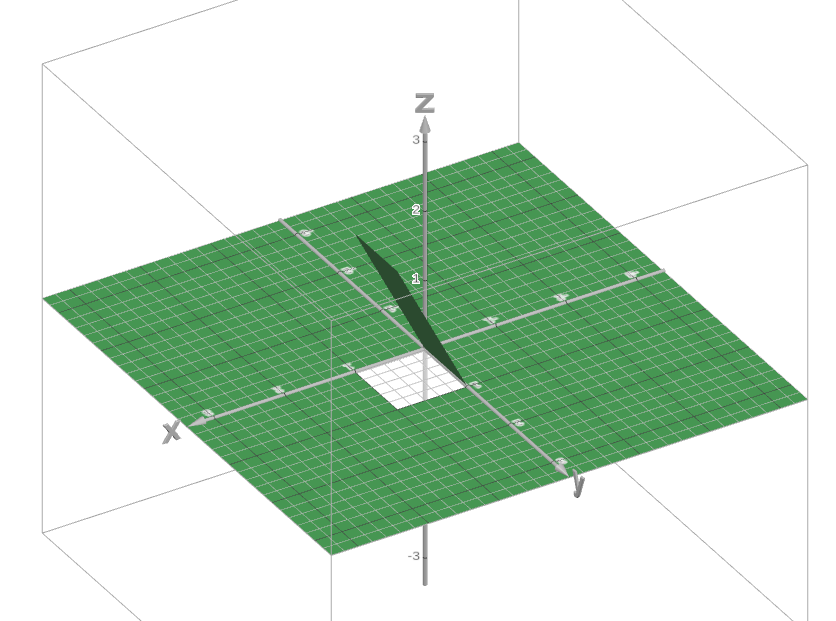
\includegraphics[scale=0.2]{MarginalIndependenceGraphChapE.png}
        \end{figure}
    \item By definition $F_X (x) = \lim_{y \ra \infty} F_{X, Y} (x, y)$. Since $X$ and $Y$ are jointly continuous, we have
        \[
            F_X (x) = \lim_{y \ra \infty} \int_{-\infty}^x \int_{-\infty}^y f_{X, Y} (u, v) \, dv du .
        \]
    When $x < 0$, we have $F_X (x) = 0$. For $0 \leq x \leq 1$, we have $f_{X, Y} (x) = 2x$, if $y$ is big enough, so that
        \[
            F_X (x) = \int_{0}^x \int_0^1 2u \, dv du = x^2 .
        \]
    When $x > 1$ and $y$ is sufficiently big (in fact bigger than $1$), we see that $F_X (x) = 1$. Therefore, 
    $$
        F_X (x) = \left\lbrace \begin{matrix} 0 & x < 0 \\ x^2 & 0 \leq x \leq 1 \\ 1 & x > 1 \end{matrix} \right.
    $$
    or we can also rewrite $F_X (x) = \big( \max \{ 0, \min \{ x , 1 \} \} \big)^2$. 

    With similar calculations, we obtain
        $$ 
            F_Y (y) = \left\lbrace \begin{matrix} 0 & y < 0 \\ x & 0 \leq y \leq 1 \\ 1 & y > 1 \end{matrix} \right. 
        $$ 
    or we can write $F_Y (y) = \max \{ 0 , \min \{ y, 1 \} \}$. 
    \item Recall that $f_X = \frac{d}{dx} F_X$. Therefore, when $x < 0$ and $x > 1$, we have $f_X = 0$. When $0 < x < 1$, we have $f_X (x) = 2x$. Similarly, we have $f_Y = \frac{d}{dy} F_Y$. Therefore, when $y < 0$ and $y > 1$, we have $f_Y = 0$. When $0 < y < 1$, we have $f_Y (y) = 1$. Remarkably, we get
        \[
            f_{X, Y} (x, y) = f_X (x) f_Y (y) !! \tag*{$\triangle$}
        \]
\end{enumerate}
\end{sol*}

\begin{theorem}
Jointly continuous random variables $X$ and $Y$ are independent if and only if there are two functions $g, h : \mR \ra [0 , \infty )$ such that
    \[
        f_{X, Y} (x, y) = g(x) h(y) \quad \forall x, y \in \mR .
    \]
\end{theorem}

\underline{\textbf{Remark:}} 
    \begin{itemize}
        \item The functions $g$ and $h$ are called the \underline{marginal probability density functions} of the random vector $(X, Y)$. 
        \item The function $g$ is equal to $f_X$, the probability density function of $X$.
        \item The function $h$ is equal to $f_Y$, the probability density function of $Y$.
    \end{itemize}

%\begin{example}
%Assume that $X$ and $Y$ are random variables with joint distribution function
%    \[
%        F_{X, Y} (x, y) = \left\lbrace \begin{matrix} 1 - e^{-x} - e^{-y} + e^{-x-y} & \text{if } x, y \geq 0 \\
%        0 & \text{elsewhere} \end{matrix} \right.
%    \]
%\begin{enumerate}[label=\alph*)]
%    \item Find the joint probability density function of $X$ and $Y$.
%    \item Are $X$ and $Y$ independent?
%\end{enumerate}
%\end{example}

%\begin{sol*}

%\end{sol*}

\begin{example}\label{Example:NonIndependence}
Let $X$ and $Y$ be two random variables having joint probability density function
    \[
        f_{X, Y} (x, y) = \left\lbrace \begin{matrix} 2 e^{-x - y} & \text{if } 0 < x < y \\
        0 & \text{elsewhere.} \end{matrix} \right. 
    \]
Are $X$ and $Y$ independent?
\end{example}

\begin{sol*}
The marginal density function of $X$ is given by
    \[
        f_X (x) = \int_{-\infty}^\infty f_{X, Y} (x, y) \, dy .
    \]
When $x < 0$, then $f_{X, Y} (x, y) = 0$ and so $f_X (x) = 0$. Let $x > 0$. Then, $f_{X, Y} (x, y) = 2 e^{-x - y}$ when $y > x$ and
    \[
        f_X (x) = \int_x^\infty 2e^{-x - y} \, dy = 2e^{-2x} .
    \]
Thus, $f_X (x) = 0$ if $x < 0$ and $f_X (x) = 2e^{-2x}$, if $x \geq 0$. 

The marginal density function of $Y$ is given by
    \[
        f_Y (y) = \int_{-\infty}^\infty f_{X, Y} (x, y) \, dx .
    \]
When $y < 0$, then $f_{X, Y} (x, y) = 0$ and so $f_Y (y) = 0$. Let $y > 0$. Then $f_{X, Y} (x, y) = 2e^{-x - y}$ when $0 < x < y$, so that
    \[
        f_Y (y) = \int_0^y 2e^{-x - y} \, dy = 2e^{-y} (1 - e^{-y} ) .
    \]
Therefore, $f_Y (y) = 0$ when $y < 0$ and $f_Y (y) = 2e^{-y} (1 - e^{-y})$ when $y \geq 0$. 

We see that
    \[
        f_{X, Y} (x, y) \neq f_X (x) f_Y (y)
    \]
and therefore, $X$ and $Y$ are not independent. \hfill $\triangle$
\end{sol*}

\subsubsection*{Conditional Density Functions}
When we don't have any information on $X$, the marginal density function $f_Y$ of $Y$ is the average
    \[
        f_Y (y) = \int_{-\infty}^\infty f_{X, Y} (x, y) \, dx .
    \]
But, if we have information on values of $X$, we may consider $P (Y \leq y | X = x)$. However, since $P (X = x) = 0$ in the continuous case, we can't use formula $P (A|B) = P (A \cap B)/ P(B)$ to get an expression of this probability. Instead, we compute $P (Y \leq y | x \leq X \leq X + \Delta x )$, for a small $\Delta x$ and then divide by $\Delta x$. Doing so, we get that
    \begin{align*}
        F_{Y | X = x} (y) = \lim_{\Delta x \ra 0 } P (Y \leq y | x \leq X \leq x + \Delta x ) &= \lim_{\Delta x \ra 0} \frac{P (Y \leq y , x \leq X \leq x + \Delta x)}{P (x \leq X \leq x + \Delta x )} \\
        &= \lim_{\Delta x \ra 0} \frac{\int_{-\infty}^y \frac{1}{\Delta x}\int_{x}^{x + \Delta x} f_{X, Y} (u, v) \, du dv}{ \frac{1}{\Delta x}\int_x^{x + \Delta x} f_X (u) \, du} \\
        &= \int_{-\infty}^y \frac{f_{X, Y} (x, v)}{f_X (x)} \, dv .
    \end{align*}

\begin{definition}
If $X$ and $Y$ are jointly continuous random variables, then the \ul{conditional density function of $Y$ given that $X = x$} is denoted by $f_{Y|X} (\cdot | x)$ and is defined by
    \[
        f_{Y|X} (y|x) = \frac{f_{X, Y} (x, y)}{f_X (x)}
    \]
for any $y \in \mR$ and $x$ satisfying $f_X (x) > 0$. 
\end{definition}

\underline{\textbf{Remark:}} 
\begin{itemize}
    \item In the continuous case, we define
        \[
            P (Y \leq y | X = x) := \int_{-\infty}^y f_{Y|X} (v|x) \, dv .
        \]
    \item Similarly, conditioning with respect to the event $\{ Y = y \}$, then the conditional density function of $X$ given that $Y = y$ is
        \[
            f_{X|Y} (x|y) = \frac{f_{X, Y} (x, y)}{f_Y (x)} .
        \]
    \item The formulas of the conditional density are very similar to the definition of $P (A|B)$.
\end{itemize}

\begin{example}
Find $f_{X|Y}$ if $X$ and $Y$ have joint probability density function 
    \[
        f_{X, Y} (x ,y) = \left\lbrace \begin{matrix} 2 e^{-x - y} & \text{ if } 0 < x < y < \infty \\
        0 & \text{otherwise.} \end{matrix} \right.
    \]
\end{example}
\begin{sol*}
From Example \ref{Example:NonIndependence}, the density of $Y$ is
    \[
        f_Y (x) = \int_{-\infty}^\infty f_{X, Y} (x, y) \, dx = 2e^{-y} (1 - e^{-y}) .
    \]

For $y < 0$, we have $f_{X|Y} (x|y) = 0$. For $y > 0$, we have
    \[
        f_{X|Y} (x|y) = \frac{2e^{-x-y}}{2e^{-y} (1 - e^{-y})} = \frac{e^{-x}}{1 - e^{-y}} . \tag*{$\triangle$}
    \]
\end{sol*}

\section{Important Measurements}

Expectation is defined for a random variable. Therefore, we will compute the expectation of a random variable $Z = g (X, Y)$, that is
    \[
        Z (s) = g (X (s), Y (s)) \quad (s \in S ),
    \]
for some function $g : \mR \times \mR \ra \mR$.

\begin{example}
Compute the expected value of the random variable $Z = X + Y$, if $X$ and $Y$ have joint probability density function $f_{X, Y}$.
\end{example}

\begin{sol*}
By definition, the expectation of $Z$ is
    \[
        \mathrm{Exp} (Z) = \int_{-\infty}^\infty z f_Z (z) \, dz .
    \]
However, we have
    \[
        P (Z \leq z ) = P (X + Y \leq z) = \iint_A f_{X, Y} (x, y) \, dA
    \]
where $A = \{ (x, y) \, : \, x + y \leq z \}$. We therefore see that
    \[
        F_Z (z) = \int_{-\infty}^\infty \int_{-\infty}^{z - x} f_{X, Y} (x, y) \, dy dx = \int_{-\infty}^z \int_{-\infty}^\infty f_{X, Y} (u, v-u) \, du dv
    \]
after the transformation $u = x$ and $v = x + y$. Therefore, differentiating, we obtain
    \[
        f_Z (z) = \int_{-\infty}^\infty f_{X, Y} (u, z - u ) \, du .
    \]
Replacing in the formula of the expectation, we find that
    \[
        \mathrm{Exp} (Z) = \int_{-\infty}^\infty z \int_{-\infty}^\infty f_{X, Y} (u, z - u) \, du dz = \int_{-\infty}^\infty \int_{-\infty}^\infty z f_{X, Y} (u, z - u ) \, du dz . 
    \]
Now, reset $u = x$ and $y = z - u$, so that $z = x + y$ and therefore
    \[
        \mathrm{Exp} (Z) = \int_{-\infty}^\infty \int_{-\infty}^\infty (x + y) f_{X, Y} (x, y) \, dx dy . \tag*{$\triangle$} .
    \]
\end{sol*}

\begin{theorem}
If $X$ and $Y$ are random variables that are jointly continuous and if $Z = g (X, Y)$ is a continuous random variable for some function $g : \mR \times \mR \ra \mR$, then
    \[
        \mathrm{Exp} (Z) = \int_{-\infty}^\infty \int_{-\infty}^\infty g (x, y) f_{X, Y} (x, y) \, dx dy 
    \]
whenever this integral exists.
\end{theorem}

\underline{\textbf{Properties:}}
    \begin{itemize}
        \item $\mathrm{Exp} (a X + bY) = a \mathrm{Exp} (X) + b \mathrm{Exp} (Y)$.
        \item If $X$ and $Y$ are independent random variable, then
            \[
                \mathrm{Exp} (X Y) = \mathrm{Exp} (X) \mathrm{Exp} (Y) .
            \]
    \end{itemize}

\begin{example}
Let $X, Y$ be two uniformly distributed on the unit disc, so that
    \[
        f_{X, Y} (x, y) = \left\lbrace \begin{matrix} \pi^{-1} & \text{if } x^2 + y^2 \leq 1 \\
        0 & \text{otherwise} \end{matrix} \right.
    \]
Find $\mathrm{Exp} (\sqrt{X^2 + Y^2})$.
\end{example}

\begin{sol*}
Here, $Z = \sqrt{X^2 + Y^2}$, so that $g (x, y) = \sqrt{x^2 + y^2}$. Applying the formula of the expectation, we find
    \[
        \mathrm{Exp} (Z) = \int_{-\infty}^\infty \int_{-\infty}^\infty \sqrt{x^2 + y^2} f_{X, Y} (x, y) \, dx dy .
    \]
Since $f_{X, Y} (x, y) = 0$ when $x^2 + y^2 > 1$, then
    \[
        \mathrm{Exp} (Z) = \iint_{D} \frac{\sqrt{x^2 + y^2}}{\pi} \, dA 
    \]
where $D = \{ (x, y) \, : \, x^2 + y^2 \leq 1 \}$. Using polar coordinates $x = r \cos \theta$ and $y = r \sin \theta$, we get
    \[
        \mathrm{Exp} (X) = \int_0^{2\pi} \int_0^1 \frac{r^3}{\pi} \, dr d\theta = \frac{1}{2} . \tag*{$\triangle$}
    \]
\end{sol*}

\subsection*{Covariance}

Recall that if $X$ and $Y$ are independent, then
    \[
        \mathrm{Exp} (XY) = \mathrm{Exp} (X) \mathrm{Exp} (Y) .
    \]
An interpretation of the last identity is that no information of $X$ and $Y$ mixed up the expectation of $XY$. We would like a measurement of how a random variable $X$ affects the outcome of another variable $Y$. In other words, we want to measure how $X$ and $Y$ are correlated!

\begin{definition}
The \underline{covariance} of the random variables $X$ and $Y$ is the quantity denoted $\mathrm{Cov} (X, Y)$ and given by
    \[
        \mathrm{Cov} (X, Y) = \mathrm{Exp} ( (X - \mu_X ) (Y - \mu_Y)),
    \]
where $\mu_X = \mathrm{Exp} (X)$ and $\mu_Y = \mathrm{Exp} (Y)$.
\end{definition}

\underline{\textbf{Remarks:}}
    \begin{itemize}
        \item The $\mathrm{Cov} (X, Y)$ depends upon the scale of measurement. This is why, in practice, we normalize to obtain the correlation (coefficient):
            \[
                \rho (X, Y) = \frac{\mathrm{Cov} (X, Y)}{\sigma_X \sigma_Y},
            \]
        where $\sigma_X = \sqrt{\mathrm{Var} (X)}$ and $\sigma_Y = \sqrt{\mathrm{Var} (Y)}$. In this case, $\rho \in [-1, 1]$. 
        \item When $\rho (X, Y) \neq 0$ it means there is a linear dependence between $X$ and $Y$, getting stronger as $\rho$ gets closer and closer to $-1$ or $1$. We have two different types of correlation between $X$ and $Y$:
            \begin{enumerate}[label=\arabic*)]
                \item $\rho (X, Y) > 0$, then when $X$ increases, then $Y$ increases.
                \item $\rho (X, Y) < 0$, then when $X$ increases, then $Y$ decreases.
            \end{enumerate}
    \end{itemize}

\begin{theorem}
If $X$ and $Y$ are random variables with means $\mu_X$ and $\mu_Y$, respectively, then
    \[
        \mathrm{Cov} (X, Y) = \mathrm{Exp} (XY) - \mathrm{Exp} (X) \mathrm{Exp} (Y) .
    \]
\end{theorem}

\begin{example}
Assume that $X$ and $Y$ are uniformly distributed on the triangle with vertices $(-1,0)$, $(0,1 )$, and $(1, 0)$. 
    \begin{enumerate}[label=\alph*)]
        \item Find $\mathrm{Cov} (X, Y)$.
        \item Are $X$ and $Y$ independent?
    \end{enumerate}
\end{example}

\begin{sol*}
    \begin{enumerate}[label=\alph*)]
        \item The joint density function of $X$ and $Y$ are
            \[
                f_{X, Y} (x, y) = \left\{ \begin{matrix} 1 & \text{ if } y-1 \leq x \leq 1 - y , \, 0 \leq y \leq 1 \\ 
                0 & \text{ elsewhere} \end{matrix} \right. 
            \]
        Using the formula for the expected value of the random variable $Z = XY$, we get
            \begin{align*}
                \mathrm{Exp} (XY) &= \int_{-\infty}^\infty \int_{-\infty}^\infty xy f_{X, Y} (x, y) \, dx dy \\ 
                &= \int_{0}^1 \int_{y-1}^{1-y} xy \, dxdy = 0 .
            \end{align*}
        After some calculations, we find that
            \[
                f_X (x) = \int_{-\infty}^\infty f_{X, Y} (x, y) \, dy = \left\lbrace \begin{matrix} 1 + x & \text{ if } -1 < x < 0 \\
                1 - x & \text{ if } 0 < x < 1 \\ 
                0 & \text{ elsewhere}
                \end{matrix} \right. 
            \]
        and
            \[
                f_Y (y) = \int_{-\infty}^\infty f_{X, Y} (x, y) \, dx = \left\lbrace \begin{matrix} 2 - 2y & \text{ if } 0 < y < 1 \\ 
                0 & \text{ elsewhere.} 
                \end{matrix} \right. 
            \]
        Therefore,
            \[
                \mathrm{Exp} (X) = \int_{-\infty}^\infty x f_{X} (x) \, dx = 0
            \]
        and
            \[
                \mathrm{Exp} (Y) = \int_{-\infty}^\infty y f_Y (y) \, dy = \frac{1}{3} .
            \]
        Hence
            \[
                \mathrm{Cov} (X, Y) = \mathrm{Exp} (XY) - \mathrm{Exp} (X) \mathrm{Exp} (Y) = 0 - ( 0) \Big( \frac{1}{3} \Big) = 0 .
            \]
        \item In this case, we see that $f_{X, Y} (x, y) \neq f_X (x) f_Y (y)$ and therefore the random variables $X$ and $Y$ are not independent eventhough their covariance is $0$!
    \end{enumerate}
\end{sol*}

\underline{\textbf{Remarks:}} 
    \begin{itemize} 
    \item If $X$ and $Y$ are independent, then $\mathrm{Cov} (X, Y) = 0$.
    \item But, the fact that $\mathrm{Cov} (X, Y) = 0$ does not necessarily imply that the random variables are independent!
    \item If $X = Y$, then $\mathrm{Cov} (X, X) = \mathrm{Var} (X)$. 
    \end{itemize}

\section{Examples of Random Vectors}

\subsection*{Uniform distribution}

If $X$ and $Y$ are two jointly random variables, then they have a \underline{uniform distribution} on the square $[a, b] \times [c, d]$ if
    \[
        f_{X, Y} (x, y) = \left\lbrace \begin{matrix} \frac{1}{(b - a) (d - c)} & \text{if } (x, y) \in [a, b] \times [c, d] \\
        0 & \text{elsewhere.} \end{matrix} \right. 
    \]

For a general region $D$, two jointly random variables $X$ and $Y$ have the uniform distribution on the region $D$ if
    \[
        f_{X, Y} (x, y) = \left\lbrace \begin{matrix} \frac{1}{\mathrm{Area} (D)} & \text{if } (x, y) \in D \\ 
        0 & \text{elsewhere.} \end{matrix} \right.
    \]
The probability of the random vector $(X, Y)$ to be in a region $B \subset D$ is given by
    \[
        P ( (X, Y) \in B) =  \frac{1}{\mathrm{Area} (D)} \iint_B \, dA = \frac{\mathrm{Area} (B)}{\mathrm{Area} (D)} .
    \]

\subsection*{Bivariate Normal Distribution}

Given $\rho \in (-1, 1)$, two jointly random variables $X$ and $Y$ has a standard bivariate normal distribution if their joint density function is
    \[
        f_{X, Y} (x, y) = \frac{1}{2\pi \sqrt{1 - \rho^2}} \exp \Big( - \frac{1}{2 (1 - \rho^2)} (x^2 - 2 \rho x y + y^2 ) \Big) \quad \forall x , y \in \mR .
    \]
We can show that
    \[
        \int_{-\infty}^\infty \int_{-\infty}^\infty f_{X, Y} (x, y) \, dx dy = 1 .
    \]
and
    \begin{enumerate}[label=\arabic*)]
        \item $f_X (x) = \frac{1}{\sqrt{2\pi}} e^{-\frac{1}{2} x^2}$, for any $x \in \mR$;
        \item $f_Y (y) = \frac{1}{\sqrt{2\pi}} e^{-\frac{1}{2} y^2}$, for any $y \in \mR$.
    \end{enumerate}
This means $X$ and $Y$ has the stardard normal distribution.

The general form of the bivariate distribution is
    \[
        f_{X, Y} (x, y) = \frac{e^{-Q/2}}{2\pi \sigma_X \sigma_Y \sqrt{1 - \rho^2}}
    \]
where
    \[
        Q = \frac{1}{1 - \rho^2} \Big[ \frac{(x - \mu_X)^2}{\sigma_X^2} - 2 \rho \frac{(x - \mu_X)(y - \mu_Y)}{\sigma_X \sigma_Y} + \frac{(y - \mu_Y)^2}{\sigma_Y^2} \Big] ,
    \]
where $\mu_X = \mathrm{Exp} (X)$, $\mu_Y = \mathrm{Exp} (Y)$, $\sigma_X = \sqrt{\mathrm{Var} (X)}$, $\sigma_Y = \sqrt{\mathrm{Var} (Y)}$, and $\rho \in (-1, 1)$.

\begin{comment}

\section{Problems Set}

\subsection*{Bivariate Distributions}

\begin{problem}
Let $(X, Y)$ be a random vector with joint distribution $F_{X, Y}$. Prove that, for any $a < c$ and $b < d$,
    \[
        P (a < X \leq b , c < Y \leq d ) = F(b, d) + F(a, c) - F (a, d) - F(b, c) .
    \]
\end{problem}

\subsection*{Continuous Random Vectors}

\begin{problem}
If $(X, Y)$ are continuous random vector with joint probability density function $f_{X, Y}$. Prove that
    \[
        P (a \leq X \leq b , c \leq Y \leq d ) = P (a < X < b , c < Y < d) .
    \]
\end{problem}

\begin{problem}
If a radioactive particle is randomly located in a square of unit length, a reasonable model for the joint density function for $X$ and $Y$ (the coordinates of the location of the radioactive particle) is
    \[
        f_{X, Y} (x, y) = \left\lbrace \begin{matrix} k x y & \text{if } (x, y) \in [0, 1] \times [0, 1] \\
        0 & \text{elsewhere} \end{matrix} \right. 
    \]
\begin{enumerate}[label=\alph*)]
\item Find the value $k$ that makes this a probability density function.
\item Find the joint distribution function for $X$ and $Y$.
\item Find $P (X \leq 0.5 , Y \leq 0.75)$.
\end{enumerate}
\end{problem}

\begin{problem}
Let $(X, Y)$ denote the coordinates of a point chosen at random inside a unit circle whose center is at the origin. Their joint probability density function is
    \[
        f_{X, Y} (x, y) = \left\lbrace \begin{matrix} 1/ \pi & \text{if } x^2 + y^2 \leq 1 \\
        0 & \text{elsewhere.} \end{matrix} \right.
    \]
Find $P (X \leq Y)$. 
\end{problem}

\subsection*{Marginals and Independence}

\begin{problem}
Let $(X, Y)$ be a continuous random vector with joint probability differentiable density function $f_{X, Y}$. Show that
    \begin{enumerate}[label=\alph*)]
        \item $f_X (x) = \displaystyle\int_{-\infty}^\infty f_{X, Y} (x, y) \, dy$.
        \item $f_Y (y) = \displaystyle\int_{-\infty}^\infty f_{X, Y} (x, y) \, dx$.
    \end{enumerate}
\end{problem}

\begin{problem}
Let $X$ and $Y$ be two random variable with joint probability density function
    \[
        f_{X, Y} (x, y) = \left\lbrace \begin{matrix} 2 & 0 \leq y \leq x \leq 1 \\
                            0 & \text{elsewhere} \end{matrix} \right. 
    \]  
    \begin{enumerate}[label=\alph*)]
        \item Sketch $f_{X, Y}$.
        \item Are $X$, $Y$ independent?
    \end{enumerate}
\end{problem}

\begin{problem}
Let $X$ and $Y$ be two random variable with joint probability density function
    \[
        f_{X, Y} (x, y) = \left\lbrace \begin{matrix} (2y+ 1)/2 & (x, y) \in [0, 1] \times [0, 1] \\
                            0 & \text{elsewhere} \end{matrix} \right. 
    \]  
    \begin{enumerate}[label=\alph*)]
        \item Sketch $f_{X, Y}$.
        \item Are $X$, $Y$ independent?
    \end{enumerate}
\end{problem}

\begin{problem}
A bus arrives at a bus stop at a uniformly distributed time over the interval $0$ to $1$ hour. A passenger also arrives at the bus stop at a uniformly distributed time over the interval $0$ to $1$ hour. Assume that the arrival times of the bus and passenger are independent of one another and that the passenger will wait for up to $1/4$ hour for the bus to arrive. What is the probability that the passenger will catch the bus?
\end{problem}

%\subsection{Sums of Random Variables}

\subsection*{Important Measurements}

\begin{problem}
Prove that if $X$ and $Y$ are two independent random variables with average $\mu_X$ and $\mu_Y$, then $\mathrm{Cov} (X, Y) = 0$. 
\end{problem}

\begin{problem}
Prove that if $X$ and $Y$ are two random variables with averages $\mu_X$ and $\mu_Y$ and standard deviation $\sigma_X$ and $\sigma_Y$, then $\rho (X, Y) \in [-1, 1]$.
\end{problem}

\begin{problem}
Let $X$ and $Y$ be random variables with means $\mu_X$ and $\mu_Y$ and with variance $\sigma_X^2$ and $\sigma_Y^2$. Use the definition of the covariance to show that
    \begin{enumerate}[label=\alph*)]
        \item $\mathrm{Cov} (X, Y) = \mathrm{Cov} (Y, X)$.
        \item $\mathrm{Var} (aX + bY) = a^2 \sigma_X^2 + b^2 \sigma_Y^2 + 2 ab \mathrm{Cov} (X, Y)$. 
        \item $\mathrm{Cov} (X, X) = \sigma_X^2$.
    \end{enumerate}
\end{problem}

\begin{problem}
The random variables $X$ and $Y$ are such that $\mathrm{Exp} (X) = 4$, $\mathrm{Exp} (Y) = -1$, $\sigma_X^2 = 2$ and $\sigma_Y^2 = 8$.
    \begin{enumerate}[label=\alph*)]
            \item What is $\mathrm{Cov} (X, X)$?
            \item What is the largest possible value for $\mathrm{Cov} (X, Y)$?
    \end{enumerate}
\end{problem}


\section{Solutions to Problems Set}
\setcounter{problem}{0} 

\subsection*{Bivariate Distributions}

\begin{problem}
See Example \ref{Ex:JointDensityRadioactiveParticle}\ref{Ex:PartcOfRadioActiveParticle}.
\end{problem}

\subsection*{Continuous Random Vectors}

\begin{problem}
Let $R = [a, b] \times [c, d]$. Then, we have
    \[
        P (a \leq X \leq b , c \leq Y \leq d ) = \iint_R f_{X, Y} (x, y) \, dA = \int_c^d \int_a^b f_{X, Y} (x, y) \, dx dy
    \]
Notice that, for any positive integer $n$,
    \[
        P (X = a , c \leq Y \leq d ) = \lim_{n \ra \infty} P (a \leq X \leq a + \frac{1}{n}, c \leq Y \leq d )
    \]
by the continuity of probability measure. Therefore, 
    \[
        P (X = a , c \leq Y \leq d ) = \lim_{n \ra \infty} \int_c^d \int_a^{a + \frac{1}{n}} f_{X, Y} (x, y) \, dx dy = \int_c^d \int_a^a f_{X, Y} (x, y) \, dx dy = 0 .
    \]
By performing similar calculations, we have $P (a \leq X \leq b , Y = c ) = 0$. 

Now, we have    
    \[
        R = (\{ a \} \times [c, d] ) \cup ( \{ b \} \times [c, d] ) \cup ( [a, b] \times \{ c \} ) \cup ([a, b] \times \{ d \} ) \cup \big( (a, b) \times (c, d) \big)
    \]
and therefore
    \begin{align*}
        P (a \leq X \leq b , c \leq Y \leq d ) &= P (X = a , c \leq Y \leq d ) + P (X = b , c \leq Y \leq d )  \\ 
        & \quad + P (a \leq X \leq b , Y = c) + P (a \leq X \leq b , Y = d ) \\ 
        & \quad + P (a < X < b , c < Y < d ) \\ 
        &= 0 + 0 + 0 + 0 + P (a < X < b , c < Y < d ) \\ 
        &= P (a < X < b , c < Y < d ) . \tag*{$\square$}
    \end{align*}
\end{problem}

\begin{problem}
\begin{enumerate}[label=\alph*)]
\item We must have
    \[
        \int_{-\infty}^\infty \int_{-\infty}^\infty f_{X, Y} (x, y) \, dx dy = 1 .
    \]
Therefore, replacing $f_{X, Y}$ by its expression, we find that it must satisfies
    \[
        \int_0^1 \int_0^1 k xy \, dx dy = 1 \quad \iff \quad \frac{k}{4} = 1 \quad \iff \quad k = 4 .
    \]
\item If $x < 0$, then $F_{X, Y} (x, y) = 0$. If $y < 0$, then $F_{X, Y} (x, y) = 0$ because $f_{X, Y} (x, y)= 0$ there. 

So, assume that $x \geq 0$ and $y \geq 0$. There are four cases to consider.
    \begin{enumerate}[label=\arabic*.]
        \item Assume $0 \leq x \leq 1$ and $0 \leq y \leq 1$. In that case, we get
            \[
                F_{X, Y} (x, y) = \int_0^y \int_0^x 4 uv \, du dv = x^2 y^2 .
            \]
        \item Assume $0 \leq x \leq 1$ and $y > 1$. In that case, we get
            \[
                F_{X, Y} (x, y) = \int_0^1 \int_0^x 4 uv \, du dv = x^2 .
            \]
        \item Assume $x > 1$ and $0 \leq y \leq 1$. In that case, we get
            \[
                F_{X, Y} (x, y) = \int_0^y \int_0^1 4uv \, du dv = y^2 .
            \]
        \item Assume $x > 1$ and $y > 1$. In that case, we get
            \[
                F_{X, Y} (x, y) = \int_0^1 \int_0^1 4uv \, du dv = 1 .
            \]
    \end{enumerate}
Hence, the joint distribution of $X$ and $Y$ is
    \[
        F_{X, Y} (x, y) = \left\lbrace \begin{matrix} x^2 y^2 & 0 \leq x \leq 1 , 0 \leq y \leq 1 \\ 
        x^2 & 0 \leq x \leq 1 , y > 1 \\ 
        y^2 & x > 1 , 0 \leq y \leq 1 \\ 
        1 & x > 1 , y > 1 \\ 
        0 & \text{elsewhere.} \end{matrix} \right. 
    \]
\item Find $P (X \leq 0.5 , Y \leq 0.75)$. Since $(0.5, 0.75) \in [0, 1] \times [0, 1]$, we obtain from (b),
    \[
        P (X \leq 0.5 , Y \leq 0.75) = F_{X, Y} (0. 5, 0.75) = (0.5)^2 (0.75)^2 = \frac{9}{64} . \tag*{$\square$}
    \]
\end{enumerate}
\end{problem}

\begin{problem}
We have $\{ X \leq Y \} = \{ (X, Y) \, : \, X \leq Y \}$. Let $R = \{ (x, y) \, : \, x \leq y \}$. Therefore,
    \[
        P (X \leq Y ) = P ( (X, Y) \in R ) = \iint_R f_{X, Y} (x, y) \, dA = \iint_{D \cap R} \frac{1}{\pi} \, dA = \frac{\mathrm{Area} (D \cap R )}{\pi} .
    \]
Notice that $D \cap R = \{ (r, \theta ) \, : \, 0 \leq r \leq 1 , \pi/4 \leq \theta \leq 5 \pi / 4 \}$ and this is half of the region inside a circle of radius $1$. Hence
    \[
        P (X \leq Y ) = \frac{\frac{\pi}{2}}{\pi} = \frac{1}{2} . \tag*{$\square$}
    \]

\end{problem}

\subsection*{Marginals and Independence}

\begin{problem}
    \begin{enumerate}[label=\alph*)]
        \item The distribution function of $X$ is given by $F_X (x) = \lim_{y \ra \infty} F_{X, Y} (x, y)$. Using the fact that $X, Y$ jointly continuous, we get
            \[
                F_X (x) = \int_{-\infty}^x \int_{-\infty}^\infty f_{X, Y} (u, y ) \, dy du .
            \]
        Taking the derivative, we get
            \[
                f_X (X) = \int_{-\infty}^\infty f_{X, Y} (x, y) \, dy .
            \]
        \item The distribution function of $Y$ is given by $F_Y (y) = \lim_{x \ra \infty} F_{X, Y} (x, y)$. Using the fact again that $X, Y$ are jointly continuous, we get
            \[
                F_Y (y) = \int_{-\infty}^y \int_{-\infty}^\infty f_{X, Y} (x, v ) \, dx dv .
            \]
        Taking the derivative, we get
            \[
                f_Y (y) = \int_{-\infty}^\infty f_{X, Y} (x, y) \, dx . \tag*{$\square$}
            \]
    \end{enumerate}
\end{problem}


\begin{problem}
    \begin{enumerate}[label=\alph*)]
        \item Below is a sketch of the density function using Desmos.
            \begin{center}
            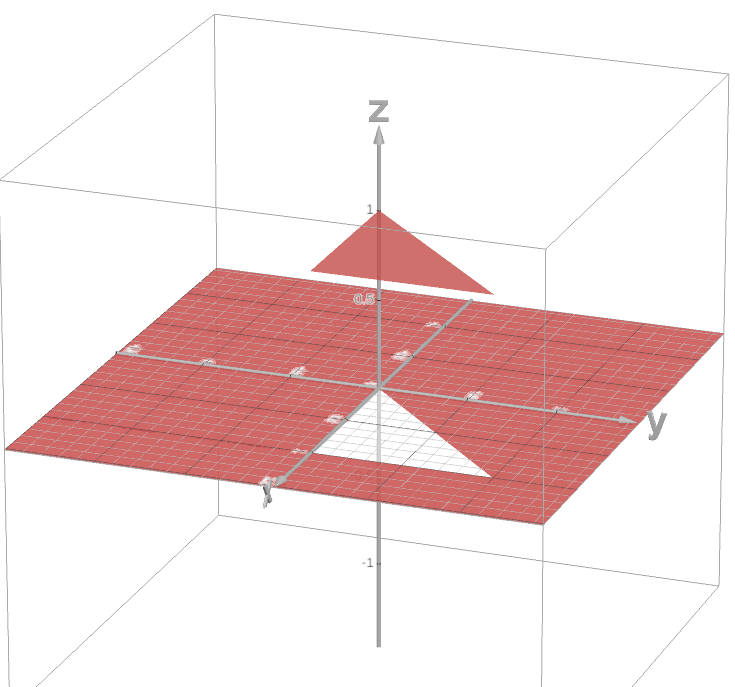
\includegraphics[scale=0.3]{figure1.png}
            \end{center}
        \item After some calculations, we get
            \[
                f_X (x) = \left\lbrace \begin{matrix} x & 0 \leq x \leq 1 \\ 0 & \text{elsewhere.} \end{matrix} \right.
            \]
        and
            \[
                f_Y (y) = \left\lbrace \begin{matrix} 1 - y & 0 \leq y \leq 1 \\ 0 & \text{elsewhere.} \end{matrix} \right. 
            \]
        We see that $f_{X, Y} (x, y) \neq f_X (x) f_Y (y)$ and therefore $X$ and $Y$ are dependent. \hfill $\square$
    \end{enumerate}
\end{problem}

\begin{problem}
    \begin{enumerate}[label=\alph*)]
        \item Below is a sketch of the density function using Desmos.
            \begin{center}
            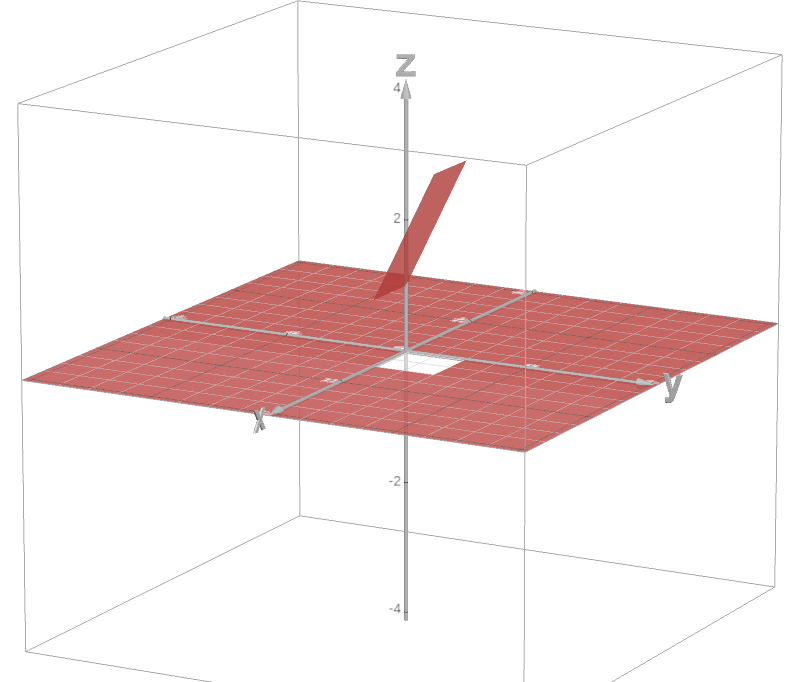
\includegraphics[scale=0.3]{figure2.png}
            \end{center}
        \item After some calculations, we get
            \[
                f_X (x) = \left\lbrace \begin{matrix} 1 & 0 \leq x \leq 1 \\ 0 & \text{elsewhere.} \end{matrix} \right.
            \]
        and
            \[
                f_Y (y) = \left\lbrace \begin{matrix} y + 1/2 & 0 \leq y \leq 1 \\ 0 & \text{elsewhere.} \end{matrix} \right. 
            \]
        We see that $f_{X, Y} (x, y) = f_X (x) f_Y (y)$ and therefore $X$ and $Y$ are independent. \hfill $\square$
    \end{enumerate}
\end{problem}

\begin{problem}
Let $X$ be the time of arrival of the passenger and let $Y$ be the time of arrival of the bus. We have $0 \leq X \leq 60$ and $0 \leq Y \leq 60$. Also, $X , Y \sim U (0, 60)$. Since there are independent, their joint density function is 
    \[
        f_{X, Y} (x, y) = f_X (x) f_Y (y) = \left\lbrace \begin{matrix} \frac{1}{3600} & (x, y) \in [0, 1] \times [0, 1] \\ 0 & \text{elsewhere} . \end{matrix} \right. 
    \]
Let $a$ be the arrival time of the passenger at the bus station. Since the passenger waits 15min for a bus to arrive, the bus must stops at the bus station between $a$min and $(a + 15)$min. Therefore, the probability is
    \[
        P (a \leq X \leq a + 15 , a \leq Y \leq a + 15 ) = \frac{15 \cdot 15}{3600} = \frac{25}{400} = \frac{1}{16} = 0.0625 . \tag*{$\square$}
    \]
\end{problem}

%\subsection{Sums of Random Variables}

\subsection*{Important Measurements}

\begin{problem}
Since $X$ and $Y$ are independent, then
    \[
        \mathrm{Cov} (X, Y) = \mathrm{Exp} (X Y) - \mathrm{Exp} (X) \mathrm{Exp} (Y) = 0
    \]
because $\mathrm{Exp} (XY) = \mathrm{Exp} (X) \mathrm{Exp} (Y)$.
\end{problem}

\begin{problem}
In this case, we need the Cauchy Schwarz inequality:
    \[
        |\mathrm{Exp} (XY)| \leq \sqrt{\mathrm{Exp} (X^2)} \sqrt{\mathrm{Exp} (Y^2)} .
    \]
Using that, we see that
    \[
        |\mathrm{Cov} (X, Y)| = \mathrm{Exp} ( (X - \mu_X ) (Y- \mu_Y)) \leq \sqrt{\mathrm{Exp} ( (X-\mu_X)^2)} \sqrt{\mathrm{Exp} ( (Y - \mu_Y)^2)} = \sigma_X \sigma_Y .
    \]
Therefore,
    \[
        |\rho (X, Y) | = \left| \frac{\mathrm{Cov} (X, Y)}{\sigma_X \sigma_Y} \right| \leq 1 . \tag*{$\square$}.
    \]
\end{problem}

\begin{problem}
    \begin{enumerate}[label=\alph*)]
        \item By definition,
            \[
                \mathrm{Cov} (X, Y) = \mathrm{Exp} ( (X -\mu_X) (Y - \mu_Y)) = \mathrm{Exp} ( (Y- \mu_Y) (X - \mu_X )) = \mathrm{Cov} (Y, X) .
            \]
        \item By the formula of the variance,
            \begin{align*}
                \mathrm{Var} (aX + bY) &= \mathrm{Exp} ( (aX + bY)^2)) - (\mathrm{Exp} (aX + bY))^2 \\ 
                &= a^2 \mathrm{Exp} (X^2) + 2ab \mathrm{Exp} (XY) + b^2 \mathrm{Exp} (Y^2) - a^2\mu_X^2 - 2ab \mu_X \mu_Y - b^2 \mu_Y^2 \\ 
                &= a^2 (\mathrm{Exp} (X^2) - \mu_X^2) + b^2 (\mathrm{Exp} (Y^2) - \mu_Y^2) + 2ab (\mathrm{Exp} (XY) - \mu_X \mu_Y ) \\ 
                &= a^2 \mathrm{Var} (X) + b^2 \mathrm{Var} (Y) + 2ab \mathrm{Cov} (X, Y) . 
            \end{align*} 
        \item By definition,
            \[
                \mathrm{Cov} (X, X) = \mathrm{Exp} ( (X - \mu_X) (X - \mu_X )) = \mathrm{Var} (X) . \tag*{$\square$}
            \]
    \end{enumerate}
\end{problem}

\begin{problem}
    \begin{enumerate}[label=\alph*)]
            \item Since $\mathrm{Cov} (X, X) = \mathrm{Var} (X)$, we find that $\mathrm{Cov} (X, X) = 2$. 
            \item Since $\rho (X, Y) \in [-1, 1]$, we see that
                \[
                    \frac{\mathrm{Cov} (X, Y)}{\sigma_X \sigma_Y} \leq 1 \quad \Rightarrow \quad \mathrm{Cov} (X, Y) \leq (\sqrt{2}) (2\sqrt{2}) = 4 . \tag*{$\square$}
                \]
    \end{enumerate}
\end{problem}

\end{comment}

%%%%%%%%%%%%%%%%%%%%%%%%%%%%%%%%%%%%%%%%
%%%%%%%%%%%% CHAPTER F %%%%%%%%%%%%%%%%%

\chapter{Moments}

In this chapter, we assume that a probability space $(S, \mathcal{A}, P)$ is given.

\section{Moments}

\begin{definition}
If $X$ is a random variable, then the $k$-th moment, with $k \geq 0$ an integer, is given by
    \[
        M_k := \mathrm{Exp} (X^k ) ,
    \]
if the expectation exists.
\end{definition}

When $X$ is a continuous random variable with pdf $f_X$, then
    \[
        M_k = \int_{-\infty}^\infty x^k f_X (x) \, dx .
    \]

\begin{example}
If $X \sim U (a, b)$, then
    \[
        M_k = \int_a^b x^k \, dx = \frac{b^{k + 1} - a^{k + 1}}{k + 1} . \tag*{$\triangle$}
    \]
\end{example}

\begin{definition}
If $X$ is a random variable with mean $\mu_X$, then the $k$-th centered moment, with $k \geq 0$ an integer is given by
    \[
        CM_k := \mathrm{Exp} ( (X - \mu_X)^k) ,
    \]
if the expected value exists.
\end{definition}

The variance of $X$ is the second centered moment of a random variable. Notice also that the $\mathrm{Var} (X)$ can be rewritten as a polynomial expression involving only $M_k$:
    \[
        \mathrm{Var} (X) = \mathrm{Exp} (X^2) - (\mathrm{Exp} (X))^2 = M_2 - (M_1)^2 .
    \]

\section{Moment Generating Function}

Notice that, if all the moments of a continuous random variable $X$ exist, then
    \[
        \sum_{k = 0}^\infty \frac{t^k}{k!} \mathrm{Exp} (X^k) ,
    \]
may exists for a certain value of $t > 0$ (and therefore for any value less than $t$). If this happens, then
    \[
        \sum_{k = 0}^\infty \frac{t^k}{k!} \mathrm{Exp} (X^k) = \int_{-\infty}^\infty \sum_{k = 0}^\infty \frac{t^k x^k}{k!} f_X (x) \, dx = \int_{-\infty}^\infty e^{tx} f_X (x) \, dx = \mathrm{Exp} (e^{tX}) .
    \]
The expectation on the right-hand side is called the \textbf{moment generating function} of $X$ and is denoted by $M_X (t)$. 

\begin{example}
If $X$ has the exponential distribution with parameter $\lambda$, then $f_X (x) = \lambda e^{-\lambda x}$ for $x \geq 0$ so that
    \[
        M_X (t) = \int_0^\infty e^{tx} \lambda e^{-\lambda x} \, dx .
    \]
If $t < \lambda$, then $(t - \lambda ) x < 0$ for any $x > 0$. Therefore, the above integral does exists with $t < \lambda$ and
    \[
        M_X (t) = \frac{\lambda}{\lambda - t} .
    \]
When $t > \lambda$, then
    \[
        M_X (t) = \infty .
    \] 
The moment generating function $M_X$ only exists when $t < \lambda$. \hfill $\triangle$
\end{example}

\begin{example}
Ìf $X$ has the normal distribution with mean $0$ and variance $1$, then
    \[
        M_X (t) = \int_{-\infty}^\infty e^{tx} \frac{1}{\sqrt{2\pi}} e^{-\frac{1}{2} x^2} \, dx = e^{\frac{1}{2} t^2} .
    \]
Using the fact that $e^t = 1 + t + t^2/2 + t^3/3! + \ldots$, we obtain
    \[
        M_X (t) = 1 + \frac{1}{2} t^2 + \frac{1}{8} t^4 + \frac{1}{8 \cdot 3!} t^6 + \ldots . \tag*{$\triangle$} 
    \]
\end{example}

The moment generating function is really useful to find the moments of a random variable.

\begin{theorem}\label{T:MomentsAndMomentGeneratingFunction}
If $M_X (t)$ exists in a neighborhood of $0$, then, for $k = 1 , 2 , \ldots$
    \[
        \mathrm{Exp} (X^k) = M_X^{(k)} (0).
    \]
\end{theorem}

\begin{example}
Let $X$ be a random variable with the exponentital distribution of parameter $\lambda >0$. Compute $M_3$. 
\end{example}

\begin{sol*}
From the previous examples, we have $M_X (t) = \frac{\lambda}{\lambda - t}$, for $t < \lambda$. We have
    \[
        M_X'(t) = \frac{\lambda}{(\lambda-t)^2}, \quad M_X'' (t) = \frac{2 \lambda}{(\lambda - t)^3} \quad \text{ and } \quad M_X^{(3)} (t) = \frac{6\lambda}{(\lambda - t)^4} .
    \]
Therefore, 
    \[
        M_3 = M_X^{(3)} (0) = \frac{6\lambda}{(\lambda - 0)^4} = 6 \lambda^{-3} . \tag*{$\triangle$}
    \]
\end{sol*}

\begin{theorem}\label{Thm:MomentGeneratingOfSum}
If $X$ and $Y$ are independent random variables, then $X + Y$ has moment generating function
    \[
        M_{X + Y} (t) = M_X (t) M_Y (t) .
    \]
\end{theorem}
\begin{proof}
Since $X$ and $Y$ are independent, we have $f_{X, Y} (x, y) = f_X (x) f_Y (y)$. Hence, 
    \begin{align*}
        M_{X + Y} (t) = \mathrm{Exp} (e^{t (X + Y)}) &= \int_{-\infty}^\infty \int_{-\infty}^\infty e^{t (x + y)} f_{X, Y} (x, y) \, dx dy \\ 
        &= \int_{-\infty}^\infty \int_{-\infty}^\infty e^{tx} f_X (x) e^{ty} f_Y (y) \, dx dy \\ 
        &= \mathrm{Exp} (e^{tX}) \mathrm{Exp} (e^{tY}) . \qedhere
    \end{align*}
\end{proof}

\begin{theorem}
Let $X$ be a continuous random variable. Assume the generating function $M_X$ satisfies $M_X (t) = \mathrm{Exp} (e^{tX})$ for all $t$ with $-\delta < t \leq \delta$ and for some $\delta > 0$. Then
    \begin{enumerate}[label=\alph*)]
         \item There is a unique distribution with moment generating function $M_X$.
         \item Furthermore, under these conditions, we have that $\mathrm{Exp} (X^k) < \infty$ for any $k = 1, 2, \ldots$ and
            \[
                M_X (t) = \sum_{k = 0}^\infty \frac{t^k}{k!} \mathrm{Exp} (X^k ) \quad |t| < \delta .
            \]
     \end{enumerate} 
\end{theorem}

\begin{example}
Let $X$ and $Y$ be independent random variables, $X \sim N (\mu_X , \sigma_X )$ and $Y \sim N (\mu_Y , \sigma_Y )$. Show that their sum $Z = X + Y$ has the normal distribution with parameters $\mu_X + \mu_Y$ and $\sigma_X^2 + \sigma_Y^2$.
\end{example}

\begin{sol*}
Let $z = (x - \mu_X )/ \sigma_X$, then
    \begin{align*}
        M_X (t) &= \int_{-\infty}^\infty e^{tx} \frac{1}{\sqrt{2\pi \sigma_X^2}} e^{-\frac{1}{2\sigma_X^2} (x - \mu_X)^2} \, dx \\ 
        &= \int_{-\infty}^\infty e^{t (\sigma_X z + \mu_X)} \frac{1}{\sqrt{2\pi}} e^{-\frac{1}{2} z^2} \, dz \\ 
        &= e^{t \mu_X} \int_{-\infty}^\infty \frac{1}{\sqrt{2\pi}} e^{t \sigma_X z} e^{-\frac{1}{2} z^2} \, dz \\ 
        &= e^{t \mu_X + \frac{1}{2} t^2 \sigma_X^2} \int_{-\infty}^\infty \frac{1}{\sqrt{2\pi}} e^{-\frac{1}{2} (z - t \sigma_X)^2} \, dz
    \end{align*}
and hence $M_X (t) = \exp (t \mu_X + \frac{1}{2} t^2 \sigma_X^2 )$. Similarly, we have $M_Y (t) = \exp (t \mu_Y + \frac{1}{2} t^2 \sigma_Y^2 )$. Therefore, by Theorem \ref{Thm:MomentGeneratingOfSum},
    \[
        M_{X + Y} (t) = M_X (t) M_Y (t) = \exp \Big(t (\mu_X + \mu_Y) + \frac{1}{2} t^2 (\sigma_X^2 + \sigma_Y^2 )\Big) .
    \]
By uniqueness of the moment generating function, we see that 
    \begin{equation}
        X + Y \sim N (\mu_x + \mu_Y , \sigma_X^2 + \sigma_Y^2 ).  \tag*{$\triangle$}
    \end{equation}
\end{sol*}

\begin{comment}

\section{Problems Set}

\subsection*{Moments}

\begin{problem}
If $X$ is uniformly distributed on $(a, b)$, show that
    \[
        \mathrm{Exp} (X^k) = \frac{b^{k + 1} - a^{k + 1}}{(b - a) (k + 1)} \quad \text{ for } k = 1, 2, \ldots .
    \]
\end{problem}

\subsection*{Moment Generating Function}

\begin{problem}
If $X$ has the normal distribution with mean $0$ and variance $1$, find $\mathrm{E} (X^3)$. 
\end{problem}

\begin{problem}
Show that, if $X$ has a normal distribution, then so does $aX + b$, for any $a, b \in \mR$ with $a \neq 0$.
\end{problem}

%\begin{problem}
%Identify the distribution of the random variables with the following moment-generating functions:
%   \begin{enumerate}[label=\alph*)]
%   \item $M (t) = (1 - 4t)^{-2}$.
%   \item $M (t) = 1/ (1 - 3.2t)$.
%   \item $M (t) = e^{-5t + 6t^2}$. 
%   \end{enumerate}
%\end{problem}

\begin{problem}
Suppose that the waiting time for the first customer to enter a retail shop after 9:00\textsc{am} is a random variable $X$ with an exponential density function given by
    \[
        f(x) = \left\{ \begin{matrix} (1/\theta ) e^{-x/\theta} & x > 0 , \\ 
        0 & \text{ elsewhere.} \end{matrix} \right.
    \]
    \begin{enumerate}[label=\alph*)]
    \item Find the moment-generating function of $X$.
    \item Use the answer from part (a) to find $\mathrm{Exp} (X)$ and $\mathrm{Var} (X)$.
    \end{enumerate}
\end{problem}



\section{Solutions to Problems Set}
\setcounter{problem}{0} 

\subsection*{Moments}

\begin{problem}
From the definition of the $k$-th moment, we compute
    \[
        \mathrm{Exp} (X^k) = \int_{-\infty}^\infty x^k f_X (x) \, dx = \int_a^b \frac{x^k}{b - a} \, dx .
    \]
After integrating $x^k$, we obtain the answer:
    \[
        \mathrm{Exp} (X^k) = \frac{b^{k + 1} - a^{k + 1}}{(k + 1) (b - a)} . \tag*{$\triangle$}
    \]
\end{problem}

\subsection*{Moment Generating Function}

\begin{problem}
The moment generating function of the normal distribution is
    \[
        M_X (t) = e^{\mu_X t + \frac{1}{2}\sigma_X^2 t^2} .
    \]
Since $\mu_X = 0$ and $\sigma_X^2 = 1$, we then get $M_X (t) = e^{t^2/2}$. From Theorem \ref{T:MomentsAndMomentGeneratingFunction}, we know that
    \[
        \mathrm{Exp} (X^3 ) = M_X^{(3)} (0) .
    \]
We have
    \[
        M_X^{(3)} (t) = e^{t^2/2} t (t^2 + 3) \quad \Rightarrow \quad \mathrm{Exp} (X^3) = 0 .\tag*{$\triangle$}
    \]
\end{problem}

\begin{problem}
We will identify the moment generating function of $aX + b$. From the definition of the moment generating function, we have
    \[  
        M_{aX + b} (t) = \mathrm{Exp} (e^{t(aX + b)}) = e^{tb} \mathrm{Exp} (e^{taX}) = e^{tb} M_X (at ) .
    \]
Since $X \sim N (\mu_X , \sigma_X )$, we know that $M_X (t) = e^{\mu_X t + \frac{1}{2} \sigma_X^2 t^2}$. Substituting this into the equation for $M_{aX + b} (t)$, we find that
    \[
        M_{aX + b} (t) = e^{tb} e^{\mu_X at + \frac{1}{2} \sigma_X^2 a^2 t^2} = e^{(b + \mu_X a) t + \frac{1}{2} \sigma_X^2 a^2 t^2} .
    \]
The moment generating function of $aX + b$ is then the moment generating function of a normal distribution with average $b + \mu_X a$ and variance $\sigma_X^2 a^2$. Hence, $aX + b \sim N (b + \mu_X a , \sigma_X^2 a^2 )$. \hfill $\triangle$
\end{problem}

%\begin{problem}
%Identify the distribution of the random variables with the following moment-generating functions:
%   \begin{enumerate}[label=\alph*)]
%   \item $M (t) = (1 - 4t)^{-2}$.
%   \item $M (t) = 1/ (1 - 3.2t)$.
%   \item $M (t) = e^{-5t + 6t^2}$. 
%   \end{enumerate}
%\end{problem}

\begin{problem}
    \begin{enumerate}[label=\alph*)]
        \item Since $X$ is an exponential distribution and $\lambda = 1/\theta$, we find that
            \[
                M_X (t) = \frac{1/\theta}{1/\theta - t} = \frac{1}{1 - \theta t} , 
            \]
        for $t < 1/\theta$.
        \item We know that
            \[
                \mathrm{Exp} (X) = M'_X (0) \quad \text{ and } \quad \mathrm{Var} (X) = \mathrm{Exp} (X^2) - (\mathrm{Exp} (X))^2 = M''_X (0) - (M'_X(0))^2 .
            \]
        We compute
            \[
                M_X' (t) = \frac{\theta}{(1 - \theta t)^2} \quad \text{ and } \quad M_X'' (t) = \frac{2\theta^2}{(1 - \theta t)^{3}}
            \]
        Hence
            \[
                \mathrm{Exp} (X) = \frac{\theta}{(1 - \theta (0))^2} = \theta
            \]
        and
            \[
                \mathrm{Var} (X) = \frac{2\theta^2}{(1 - \theta (0))^3} - (\theta)^2 = \theta^2 . \tag*{$\triangle$}
            \]
    \end{enumerate}
\end{problem}

\end{comment}

%%%%%%%%%%%%%%%%%%%%%%%%%%%%%%%%%%%%%%%%
%%%%%%%%%%%% CHAPTER G %%%%%%%%%%%%%%%%%
\chapter{Two Main Laws}

We assume a probability space $(S, \mathcal{A}, P)$ is given.

\section{Law of Averages}

\begin{definition}
If $x_1$, $x_2$, $\ldots$, $x_n$ are real numbers, then the average is defined by
    \[
        \sigma_n := \frac{x_1 + x_2 + \cdots + x_n}{n} .
    \]
\end{definition}

\begin{example}
We throw a fair die $10$, $20$, $40$, and $60$ times and record the result (check \url{www.rolladie.net}). Let $X_j$ be the random variable giving the number of dots of the face on which the die landed. Compute the average of the $X_j$'s. What do you observe? What number do you think the average should be close to?
\end{example}

In general, in probability, we would like a theorem telling us something like ``if we repeat an experiment many times, then the average of the results approaches the underlying mean value.''

\begin{definition}
We say that the sequence $X_1$, $X_2$, $\ldots$ of random variables \underline{converges in mean} \underline{square to the random variable $X$} if
    \[
        \mathrm{Exp} \big( (X_n - X)^2 \big) \ra 0 \quad \text{ as } n \ra \infty.
    \]
If this holds, then we write ``$X_n \ra X$ in mean-square as $n \ra \infty$''.
\end{definition}

\begin{theorem}[Mean-Square Law of Averages]

Let $X_1$, $X_2$, $\ldots$, $X_n$, $\ldots$ be a list of uncorrelated random variables, each having mean $\mu$ and variance $\sigma^2$. Then,
    \[
        \frac{X_1 + X_2 + \ldots + X_n}{n} \ra \mu \quad \text{(in mean-square.)}
    \]
\end{theorem}

\begin{proof}
Write $S_n = X_1 + X_2 + \ldots + X_n$. Then,
We have
    \[
        \mathrm{Exp} (S_n /n) = \frac{1}{n} \mathrm{Exp} (X_1 + X_2 + \cdots + X_n ) = \frac{1}{n}n \mu = \mu .
    \]
and
    \[
        \mathrm{Exp} \big( (\sigma_n - \mu )^2 \big) = \mathrm{Exp} \Big( \frac{(S_n - n \mu)^2}{n^2} \Big) = \frac{1}{n^2} \mathrm{Var} (S_n ) .
    \]
The random variables are uncorrelated, meaning $\mathrm{Cov} (X_i, X_j ) = 0$, for any $i \neq j$. Therefore,
    \[
        \mathrm{Var} (X_1 + X_2 + \cdots + X_n ) = \mathrm{Var} (X_1) + \mathrm{Var} (X_2) + \cdots + \mathrm{Var} (X_n ) = n \sigma^2 .
    \]
Hence,
    \[
        \mathrm{Exp} \big( (\sigma_n - \mu )^2 \big) = \frac{\sigma^2}{n} \ra 0
    \]
as $n \ra \infty$. Therefore, $\sigma_n \ra \mu$ in mean-square as $n \ra \infty$.
\end{proof}

\subsection*{Convergence in Probability}

\begin{definition}
A sequence of random variable $X_1$, $X_2$, $\ldots$ \underline{converges in probability} to a random variable $X$ if for any $\varepsilon > 0$, 
    \[
        \lim_{n \ra \infty} P (|X_n - X| > \varepsilon ) = 0 .
   \]
\end{definition}

\begin{example}
Let $X_1$, $X_2$, $\ldots$ be a sequence of discrete random variables. Assume that the probability mass function of $X_n$ is given by
    \[
        P (X_n = 0) = 1 - \frac{1}{n} \quad \text{ and } \quad P (X_n = n ) = \frac{1}{n} \quad (n \geq 1) .
    \]
Show that $X_n \ra 0$ in probability as $n \ra \infty$, but $X_n$ does not converge to $0$ in mean square as $n \ra \infty$.
\end{example}

\begin{sol*}
We start with the convergence in probability. For $\varepsilon > 0$ and for any $n > \varepsilon$, we have
    \[
        P (|X_n - 0| > \varepsilon ) = P (X_n = n) = \frac{1}{n} \ra 0 \quad (n \ra \infty ). 
    \]
This implies that $X_n \ra 0$ in probability when $n \ra \infty$. 

As for the mean square convergence, we have
    \[
        \mathrm{Exp} ( (X_n - 0)^2) = E (X_n^2) = (0) \Big( 1 - \frac{1}{n} \Big) + (n^2) \Big( \frac{1}{n} \Big) = n \ra \infty .
    \]
Hence, $X_n$ does not converge in mean square to $0$. 
\end{sol*}

\underline{\textbf{Remark:}} The last example shows that convergence in probability does not imply convergence in mean. 

On the other hand, convergence in mean does imply convergence in probability. This is Theorem \ref{T:MEanQuareImpliesProbability}. To show this result, we need an intermediate result called Chebyshev's inequality.

\begin{theorem}
If $X$ is a random variable and $\mathrm{Exp} (X^2) < \infty$, then for any $t > 0$
    \[
        P (|X| \geq t ) \leq \frac{1}{t^2} \mathrm{Exp} (X^2 ).
    \]
\end{theorem}

Here is a consequence of Chebyshev's inequality.

\begin{theorem}\label{T:MEanQuareImpliesProbability}
If a sequence of random variables $X_1$, $X_2$, $\ldots$ converges in mean-square to a random variable $X$, then it also converges in probability to $X$.
\end{theorem}
\begin{proof}
Assume that $\mathrm{Exp} ( (X_n - X)^2 ) \ra 0$, as $n \ra \infty$. Given $\varepsilon > 0$, from Chebyshev's inequality, we get that
    \[
        P (|X_n - X| > \varepsilon ) \leq \frac{1}{\varepsilon^2} \mathrm{Exp} ( (X_n - X)^2 ) 
    \]
Since $\varepsilon$ is fixed and $\lim_{n \ra \infty} \mathrm{Exp} ( (X_n - X)^2 ) = 0$, we get
    \[
        \lim_{n \ra \infty} P (|X_n - X | > \varepsilon ) = 0 . \qedhere
    \]
\end{proof}


\section{Central Limit Theorem}

Let $X_1$, $X_2$, $\ldots$ be independent random variables with the same means $\mu$ and variance $\sigma^2$. Letting $S_n = X_1 + X_2 + \ldots + X_n$, we have
    \[
        \mathrm{Exp} (S_n) = n \mu \quad \text{and} \quad \mathrm{Var} (S_n) = n \sigma^2 .
    \]
Then, define
    \[
        Z_n = \frac{S_n - \mathrm{Exp} (S_n)}{\sqrt{\mathrm{Var} (S_n)}} = \frac{S_n - n \mu}{\sqrt{n} \sigma} .
    \]
Then, $\mathrm{Exp} (Z_n) = 0$ and $\mathrm{Var} (Z_n) = 1$. These are called the \underline{standardized version} of the sum $S_n$. 

Remarkably, the sequence of random variables $Z_n$ settles to a limit as $n \ra \infty$. Even more impressive is the fact the distribution of the limit can be identified explicitly!

\begin{theorem}
Let $X_1$, $X_2$, $\ldots$ be independent and identically distributed random variables, each with mean $\mu$ and non-zero variable $\sigma^2$. The random variables $Z_n$ satisfies the following:
    \[
        P (Z_n \leq z ) \ra \int_{-\infty}^z \frac{1}{\sqrt{2\pi}} e^{-u^2/2} \, du \quad \forall z \in \mR .
    \]
\end{theorem}

We won't prove this Theorem in this class. It requires a difficult result called the \textit{Continuity Theorem}. We will therefore take for granted the Central Limit Theorem and use it in the next example.

\begin{example}
An unknown fraction $p$ of the population are jedi knights. It is desired to estimate $p$ with error not exceeding $0.005$ by asking a sample of individuals. How large a sample is needed?
\end{example}

\begin{sol*}
We use the Central Limit Theorem. Let $X_i$ be the random variable following a Bernouilli distribution, meaning $X_i = 0$ if the $i$-th person answers no and $X_i = 1$ if that same person answers yes. We have 
    \[
        \mathrm{Exp} (X_i) = p \quad \text{ and } \quad \mathrm{Var} (X_i) = p (1 - p) .
    \]

Set $S_n = X_1 + X_2 + \ldots + X_n$, where $n$ is the size of the sample of individuals. We decide to estimate $p$ with $\hat{p} = S_n /n$. Our goal is to find $n$ such that $|\hat{p} - p| < 0.005$.

The good practice is to reach our goal with a certain degree of certainty. Therefore, we want to find $n$ such 
    \[
        P ( |\hat{p} - p| > 0.005 ) < \alpha 
    \]
where $\alpha$ is called the $p$-value or the tolerance value. In practice, we use $\alpha = 0.05$. Therefore, we want to find $n$ such that 
    \[
        P (| \hat{p} - p | \leq 0.005 ) < 0.95 .
    \]

We can rewrite the previous probability as
    \[
        P (|\hat{p} - p| \leq 0.005 ) = P \left( \frac{|S_n - n p|}{\sqrt{n p (1 - p)}} \leq 0.005\frac{\sqrt{n}}{\sqrt{p (1 - p)}} \right) = P \left( |Z_n| \leq 0.005 \frac{\sqrt{n}}{\sqrt{p (1 - p)}} \right) ,
    \]
where $Z_n = \frac{S_n - \mathrm{Exp} (S_n)}{\sqrt{\mathrm{Var} (S_n)}}$. However, $p (1 - p)$ is unknown and the number $0.005 \frac{\sqrt{n}}{\sqrt{p (1 - p)}}$ is useless. We can see that $p (1 - p) \leq \frac{1}{4}$ and therefore
    \[
        P \left( |Z_n| \leq 0.005 \frac{\sqrt{n}}{\sqrt{p (1 - p)}} \right) \geq P (|Z_n| \leq 0.005 \sqrt{4n} ) .
    \]

From the Central Limit Theorem, if $n$ is large enough, then the distribution of $Z_n$ approaches the distribution of a $Z \sim N (0, 1)$.  Therefore
    \[ 
        P \left( |Z_n| \leq 0.005 \frac{\sqrt{n}}{\sqrt{p (1 - p)}} \right) \gtrapprox P (|Z| \leq 0.005 \sqrt{4n} ) = P (Z \leq 0.005 \sqrt{4n} ) - P (Z \leq -0.005 \sqrt{4n} ) .
    \]
For that probability to be bigger than $0.95$, we have to have $0.005 \sqrt{4n} \geq 1.96$, which means $n \gtrapprox 40,000$. \hfill $\triangle$
\end{sol*}


\begin{comment}

\section{Problems Set}

\subsection*{Mean-Square Law of Large Numbers}

\begin{problem}
Let $X_1, X_2, \ldots$ be a list of random variables which converges to the random variable $X$ in mean square. Show that, for any $a, b \in \mR$, $aX_n + b \ra aX + b$, as $n \ra \infty$.
\end{problem}

\begin{problem}
Let $N_m$ be the number of occurences of $5$ or $6$ in $m$ throws of a fair die. Show that
    \[
        \frac{1}{m} N_m \ra \frac{1}{3} \quad \text{ in mean square}
     \] 
as $m \ra \infty$.
\end{problem}

%\begin{problem}
%Prove the following alternative form of Chebyshev's inequality: If $X$ is a random variable with finite variance and $a > 0$, then
%    \[
%        P \big( |X - \mathrm{Exp} (X)| > a \big) \leq \frac{1}{a^2} \mathrm{Var} (X) .
%    \]
%\end{problem}

%\begin{problem}
%Show that if $X_n \ra X$ in probability, then, as $n \ra \infty$,
%    \[
%        aX_n + b \ra aX + b \quad \text{in probability},
%    \]
%for any $a, b \in \mR$.
%\end{problem}

\subsection*{Central Limit Theorem}

\begin{problem}
The fracture strength of tempered glass averages 14 (measured in thousands of pounds per square inch) and has standard deviation $2$. 
    \begin{enumerate}[label=\alph*)]
    \item What is the probability that the average fracture strength of 100 randomly selected pieces of this glass exceeds 14.5?
    \item Find an interval that includes, with probability 0.95, the average fracture strength of 100 randomly selected pieces of this glass.
    \end{enumerate}
\end{problem}

%\begin{problem}
%A fair die is thrown $12,000$ times. Use the central limit theorem to find values of $a$ and $b$ such that
%    \[
%        P (1900 < S < 2200) \approx \int_a^b \frac{1}{\sqrt{2\pi}} e^{-\frac{1}{2} x^2} \, dx ,
%    \]
%where $S$ is the total number of sixes thrown.
%\end{problem}


\section{Solutions to Problems Set}
\setcounter{problem}{0} 

\subsection*{Mean-Square Law of Large Numbers}

\begin{problem}
We have
    \[
        \mathrm{Exp} ((aX_n + b - (aX + b))^2) = \mathrm{Exp} (a^2 (X_n - X)^2) = a^2 \mathrm{Exp} ( (X_n - X)^2 ) .
    \]
By assumption, $\lim_{n \ra \infty} \mathrm{Exp} ( (X_n - X)^2) = 0$, therefore
    \[
        \lim_{n \ra \infty} \mathrm{Exp} ( (aX_n + b - (aX + b))^2) = a^2 \lim_{n \ra \infty} \mathrm{Exp} ( (X_n - X)^2 ) = 0 . 
    \]
Hence, $aX_n + b \ra aX + b$ in mean-square. \hfill $\triangle$
\end{problem}

\begin{problem}
Let $N_m$ be the number of occurences of $5$ or $6$ in $m$ throws of a fair die. Show that
    \[
        \frac{1}{m} N_m \ra \frac{1}{3} \quad \text{ in mean square}
     \] 
as $m \ra \infty$.

Let $X_i$ be the random variable with output $1$ if the die lands on $5$ or $6$ and output $0$ if the die lands on $1, 2, 3$, or $4$. Then, we have
    \[
        \mathrm{Exp} (X_i) = 0 \times \frac{2}{3} + 1 \times \frac{1}{3} = \frac{1}{3}
    \]
and
    \[
        \mathrm{Var} (X_i ) = \mathrm{Exp} (X_i^2) - (\mathrm{Exp} (X_i))^2 = \frac{1}{3} - \frac{1}{9} = \frac{2}{9} .
    \]
Therefore, we get $\mathrm{Exp} (N_m) = \frac{m}{3}$ and $\mathrm{Var} (N_m ) = \frac{2m}{9}$ because in $N_m$ are independent. Hence, we compute
    \[
        \mathrm{Exp} \Big( \Big( \frac{N_m}{m} - \frac{1}{3} \Big)^2\Big) = \mathrm{Exp} \Big( \frac{(N_m - \frac{m}{3})^2}{m^2} \Big) = \frac{1}{m^2} \mathrm{Var} (N_m) = \frac{2}{9m} .
    \]
As $m \ra \infty$, $\frac{2}{9m} \ra 0$ and therefore $N_m/m \ra 1/3$ in mean-square, as $m \ra \infty$. \hfill $\triangle$
\end{problem}

%\begin{problem}
%Prove the following alternative form of Chebyshev's inequality: If $X$ is a random variable with finite variance and $a > 0$, then
%   \[
%       P \big( |X - \mathrm{Exp} (X)| > a \big) \leq \frac{1}{a^2} \mathrm{Var} (X) .
%   \]
%\end{problem}

%\begin{problem}
%Show that if $X_n \ra X$ in probability, then, as $n \ra \infty$,
%   \[
%       aX_n + b \ra aX + b \quad \text{in probability},
%   \]
%for any $a, b \in \mR$.
%\end{problem}

\subsection*{Central Limit Theorem}

\begin{problem}

    \begin{enumerate}[label=\alph*)]
    \item Let $X_i$ be a random variable with output the facture strenght of the $i$-th piece. Then, we have $\mu = \mathrm{Exp} (X_i) = 14$, for any $i$ and $\sigma^2 = \mathrm{Var} (X_i) = 4$ for any $i$. We have $n = 100$, the size of the sample and let $S_n/n = (X_1 + X_2 + \ldots + X_n)/n$ represents the average of the fracture strength in the sample.

    We will use the Central Limit Theorem to estimate the probability
        \[
            P \Big( \frac{S_{100}}{100} > 14.5 \Big) .
        \]
    The standardized version of $S_{100}$ is 
        \[
            Z_{100} = \frac{S_{100} - 100 \mu}{\sqrt{100} \sigma} = \frac{S_{100} - 1400}{20} .
        \]
    We see that
        \[
            \frac{S_{100}}{100} > 14.5 \iff S_{100} > 1450 \iff S_{100} - 1400 > 50 \iff \frac{S_{100} - 1400}{20} > 2.5 .
        \]
    Therefore, 
        \[
            P \Big( \frac{S_{100}}{100} > 14.5 \Big) = P (Z_{100} > 2.5 ) .
        \]
    
    From the Central Limit Theorem,
        \[
            P \Big( \frac{S_{100}}{100} > 14.5 \Big) = P (Z_{100} > 2.5 ) \approx P (Z > 2.5 )
        \]
    where $Z \sim N (0, 1 )$. Using the table of the normal distribution, we find that
        \[
            P (Z > 2.5) = 1 - P (Z \leq 2.5 ) = 1 - 0.99379 = 0.00731 .
        \]
    \item Since the standardized version is centered at the average, we will try to find $a$ such that $S_n/n \in [\mu - a , \mu + a ]$ in $95\%$ of the chances. We want to find $a > 0$ such that
        \[
            P \Big( \left| \frac{S_{100}}{100} - \mu \right| < a \Big) = 0.95 .
        \]
    Rearranging the left-hand side:
        \[
            \frac{S_{100}}{100} - 14 = \frac{S_{100} - 1400}{100} = \frac{2}{10} \Big( \frac{S_{100} - 1400}{20} \Big) = \frac{2}{10} Z_n
        \]
    and therefore
        \[
            P \Big( \left| \frac{S_{100}}{100} - 1400 \right| < a \Big) = P (|Z_n| < 5a ) .
        \]
    Using the Central Limit Theorem, $P (|Z_n| < 5a ) \approx P (|Z| < 5a )$, for $Z \sim N (0, 1)$ and we have to find $a$ such that $P (|Z| < 5a ) = 0.95$. Now, since the normal density of $N (0, 1)$ is symmetric with respect to the $y$-axis, we have $P (Z > 5a ) = 0.025 = P (Z < -5a )$. Therefore, 
        \[
            P (|Z| < 5a ) = 0.95 \iff P (Z < 5a ) = 0.975 .
        \]
    Using the table, we find $z = 1.96$ and therefore $a = 1.96/5 = 0.392$. Hence, the interval containing $S_{100}/100$ in $95\%$ of the chances is $[13.608, 14.392]$. 
    \end{enumerate}
\end{problem}

\end{comment}




\newpage 
\appendix 
\addcontentsline{toc}{chapter}{Appendix}

\renewcommand{\chapterformat}[1]{%
	\ul{Appendix {\thechapter}: #1}
	}

%%%%%%%%%%%%%%%%%%%%%%%%%%%%%%%%%%%%%%%%
%%%%%%%%%%%% Logic %%%%%%%%%%%%%%%%%%%%%
\setcounter{chapter}{11}
\chapter{Logic and Proofs}%\addcontentsline{toc}{chapter}{Logic and Proofs}


\section{Mathematical Statements}

A \underline{statement} is a sentence (written in words, mathematical symbols, or a combination of the two) that is either true or false.\footnote{Most of the material presented here is from the really good notes retrieved online at \url{https://sites.math.washington.edu/~conroy/m300-general/ConroyTaggartIMR.pdf}. Some passages might entirely be copied or modified slightly from this resource.}

\begin{example}
\begin{enumerate}[label=\alph*)]
\item $4 + 11 = 15$. \\This is a statement and it is true.
\item $x > 5$.\\ This is not a statement. Grammatically, it is a complete sentence, written in mathematical symbols, with a subject ($x$) and a predicate (\textit{is greater than $5$}). The sentence, however, is neither true or false because the value of $x$ is not specified.
\item If $x = 5$, then $x > 0$. \\This is a statement and it is true.
\item There exists a positive integer $n$ such that $n > 2$.\\ This is a statement and it is true.
\item Is the number $20$ an even number? \\This is not a statement. A question is neither true or false.
\end{enumerate}
\end{example}

A \underline{proof} is a piece of writing that demonstrates that a particular statement is true. A statement that we prove to be true is often called a \underline{theorem}. A statement that we assume without proof is an \underline{axiom}. A \underline{definition} is an agreement between the writer (or professor) and the reader (or the student) as to the meaning of a word or phrase. A definition needs no proof.



\section{Logic and Mathematical Language}

In the section on set theory, you will have the chance to practice the methods of proof presented below.

\subsubsection*{Negation}
If $P$ is a statement, then it has a \underline{truth value}: true or false. The \underline{negation} of a statement $P$ is defined as \textit{it is not the case that $P$}. The negation of a statement $P$ will be abbreviated by $not\, P$ or $\neg P$.

\begin{example}
Consider the statement $P$: ``$2$ is an even integer''. The negation of $P$ is ``It is not the case that $2$ is an even integer'' that may be rewritten as ``$2$ is not an even integer''. We may even go further and rewrite $\neg P$ as follows: ``$2$ is an odd integer''. Notice that $P$ is true and $\neg P$ is false.
\end{example}

\subsubsection*{Conjunction and Disjunction}
Let's consider two statements $P$ and $Q$.

	\begin{itemize}
		\item The \underline{conjunction} of $P$ and $Q$ is the statement ``$P$ and $Q$''. It is denoted by $P \wedge Q$ and it is true only when $P$ and $Q$ are true; otherwise it is false.
		\item The \underline{disjunction} of $P$ and $Q$ is the statement ``$P$ or $Q$''. It is denoted by $P \vee Q$ and it is true when one of the two statements is true.
	\end{itemize}

We can use a truth table to illustrate the conjunction and disjunction of two statements $P$ and $Q$ as shown below.

\begin{center}
	\begin{minipage}{0.45\textwidth}
	\centering
	\begin{tabular}{c|c|c}
	$P$ & $Q$ & $P \wedge Q$ \\\hline 
	$T$ & $T$ & $T$ \\\hline 
	$T$ & $F$ & $F$ \\\hline 
	$F$ & $T$ & $F$ \\\hline 
	$F$ & $F$ & $F$ \\
	\end{tabular}\vspace*{4pt}

	(a) Truth table for $P \wedge Q$
	\end{minipage}
	\begin{minipage}{0.45\textwidth}
	\centering
	\begin{tabular}{c|c|c}
	$P$ & $Q$ & $P \vee Q$ \\\hline 
	$T$ & $T$ & $T$ \\\hline 
	$T$ & $F$ & $T$ \\\hline 
	$F$ & $T$ & $T$ \\\hline 
	$F$ & $F$ & $F$ \\
	\end{tabular}\vspace*{4pt}

	(b) Truth table for $P \vee Q$
	\end{minipage}
\end{center}

\vspace*{12pt}

\begin{example}
\begin{enumerate}[label=\alph*)]
\item Consider the statement $P$: ``$2$ is a positive integer'' and the statement $Q$: ``$-4$ is a negative integer''. The statement $P \wedge Q$ is true because $P$ and $Q$ are true. But $P \wedge (\neg Q)$ is not true because $\neg Q$: ``$-4$ is not a negative integer'' is false.
\item Consider the same statements from part a). The statement $P \vee Q$ is true because the integer $2$ is a positive integer and only one of the statements $P$, $Q$ needs to be true. The statement $(\neg P) \vee Q$ is also true because the statement $Q$ is true ($-4$ is a negative number). But the statement $(\neg P) \vee (\neg Q)$ is not true because $\neg P$ and $\neg Q$ are both false.
\end{enumerate}
\end{example}

We can take the negation of a conjunction and of a disjunction.

\begin{example}
A friend tells you the conditions to come to his party. He tells you that you must wear green clothes only AND bring a one-page explanation of why you are at his party. A person that wants to go to your friend's party must satisfies \textit{both} conditions. Anyone who is wearing a non-green piece of clothe will not be allowed at the party. Also, anyone who did not write the one-page essay will not be allowed at the party. Therefore, anyone who does not wear a green outfit or anyone who did not write the one-page essay will not come to the party. 
\end{example}

\underline{Conclusion:} The negation of $P \wedge Q$ is $(\neg P) \vee (\neg Q)$.

\begin{example}
Your friend decides to be more welcoming. He tells you the conditions to come to his party remains the same, but only one of them must be meet. In other words, you may wear green clothes only OR bring a one-page explanation of why you are at his party. A person that wants to go to your friend's party must satisfy one of the two conditions. But if the person is not dressed in green clothes and does not bring the one-page essay, then unfortunately, that person will not be allowed to join the party. In other words, if both conditions are not respected by a person, then that person will not be allowed to join the party.
\end{example}

\underline{Conclusion:} The negation of $P \vee Q$ is $(\neg P) \wedge (\neg Q)$.

\subsubsection*{Conditional}

A lot of statements we will encounter are of the form ``If $P$, then $Q$''. These statements are called \underline{conditional statements}. We will use the following notation ``$P \Rightarrow Q$'' to denote a conditional statement.

The truth value of the statement $P \Rightarrow Q$ depends on the truth values of $P$ and $Q$.

\begin{example}
We think of $P \Rightarrow Q$ as an agreement. Joe makes a deal with his parents. Let $P$: ``Joe did the dishes after dinner'' and $Q$: ``Joe got \$5''. The agreement is
	\begin{align*}
	P \Rightarrow Q : \, \text{If Joe did the dishes, then he got \$5.}
	\end{align*}
Joe is not required to do the dishes (it is a compulsory act for his love for his family, but also for his love for money). In the case that Joe did the dishes ($P$ is true) and got paid ($Q$ is true), the agreement is met ($P \Rightarrow Q$ is true). In the case that Joe didn't do the dishes ($P$ is false) and didn't get paid ($Q$ is false), the agreement is met ($P \Rightarrow Q$ is true). Since Joe is not required to wash the dishes, his parents may choose to give him \$5 for some other reason. That is, in the case Joe did not do the dishes ($P$ is false) and got \$5 anyway ($Q$ is true), the agreement is still met ($P \Rightarrow Q$ is true). The only instance in which the agreement is not met ($P \Rightarrow Q$ is false) is in the case that Joe did wash the dishes ($P$ is true), but did not get the money from his parents ($Q$ is false).
\end{example}

To summarize, the statement $P \Rightarrow Q$ is true unless $P$ is true and $Q$ is false, like it is shown in the table below.

	\begin{center}
		\begin{tabular}{c|c|c}
		$P$ & $Q$ & $P \Rightarrow Q$ \\\hline 
		$T$ & $T$ & $T$ \\\hline 
		$T$ & $F$ & $T$ \\\hline 
		$F$ & $T$ & $F$ \\\hline 
		$F$ & $F$ & $T$ \\
		\end{tabular}\vspace*{4pt}

		Truth table for the conditional
	\end{center}

To explain the negation of the conditional, we use Joe's story from the previous example. Joe claims that his parents broke their verbal contract, while the parents deny Joe's claim. In other words, Joe's parents say that $P \Rightarrow Q$ is true, while Joe says that $\neg (P \Rightarrow Q)$ is true. If you were Joe's lawyer, what evidence would you have to provide to win the case? You would need to show that Joe washed the dishes and did not get paid. That is, you would need to show that $P \wedge (\neg Q)$ is true.

	\underline{Conclusion:} The negation of the conditional statement $P \Rightarrow Q$ is the statement $P \wedge (\neg Q)$.

\subsubsection*{Converse and Contrapositive}

\begin{definition}
The \underline{converse} of $P \Rightarrow Q$ is the statement $Q \Rightarrow P$. The \underline{contrapositive} of $P \Rightarrow Q$ is the statement $(\neg Q) \Rightarrow (\neg P)$.
\end{definition}

\begin{example}
Consider the statements $P$: ``Valérie's cat is hungry'' and $Q$: ``Valérie's cat meows''. 
	\begin{itemize}
	\item The implication $P \Rightarrow Q$ reads as ``If Valérie's cat is hungry, then the cat meows''. 
	\item The converse $Q \Rightarrow P$ of $P \Rightarrow Q$ reads as ``If Valérie's cat meows, then the cat is hungry''. Notice that in this contexte, $P \Rightarrow Q$ does not have the same truth value of $Q \Rightarrow P$. For instance, the cat might moews because it wants to be pet. 
	\item The contrapositive of $P \Rightarrow Q$ reads as ``If Valérie's cat does not meow, then the cat is not hungry''. You can check that $P \Rightarrow Q$ has the same truth value of $(\neg Q) \Rightarrow (\neg P)$.
	\end{itemize}
\end{example}

\subsubsection*{Equivalent statement}

\begin{definition}
The statement $P$ if and only if $Q$, written $P \iff Q$, is readily the statement
	\begin{align*}
	(P \Rightarrow Q) \wedge (Q \Rightarrow P) .
	\end{align*}
\end{definition}

\subsubsection*{Quantifiers}

Suppose $n$ is an integer and $P(n)$ is a statement about $n$. 
	\begin{itemize}
	\item If $P (n)$ is true for at least one integer $n$, then we say ``There exists $n$ such that $P (n)$''. This type of statement is called an \underline{existence statement} and the symbol $\exists$ is used as a shortcut for the ``there exists'' part.
	\item If $P(n)$ is true no matter what value $n$ takes, then we say ``For all $n$, $P (n)$''. This type of statement is called a \underline{universal statement} and the symbol $\forall$ is used as a shortcut for the ``For all'' part.
	\end{itemize}
These statements are called \underline{quantified statements}.

\begin{example} Assume throughout this example that $n$ is an integer.
	\begin{enumerate}[label=\alph*)]
		\item ``There exists $n$ such that $n > 0$''. In this statement, $P (n)$ is ``$n > 0$. The statement $P (10)$ is true because $10 > 0$, therefore the statement ``$\exists n$ such that $n > 0$'' is true because $P (n)$ is true for at least one integer $n$.
		\item ``For all $n$, $n > 0$''. The statement $P (-1)$ is false since $-1$ is not greater than $0$. Therefore, the statement ``$\forall n$, $P (n)$'' is false because $P(n)$ is \textit{not} true for every integer $n$.
		\item ``$\exists n$ such that $|n| < 0$''. This statement is false because there is no integer $n$ with $|n| < 0$; the absolute value turns every integer into a positive or zero integer.
	\end{enumerate}
\end{example}

Here are the ways to negate a quantified statement:
\begin{itemize}
	\item The negation of ``$\exists n$ such that $P (n)$'' is ``$\forall n$, $\neg (P (n))$''.
	\item The negation of ``$\forall n$, $P(n)$'' is ``$\exists n$ such that $\neg (P (n))$``.
\end{itemize}




\section{Methods of Proof}

We will cover some methods to prove mathematical statements. The two we will cover are direct proofs of a conditional statement and proofs by contradiction.


\subsubsection*{Direct Proof}
There are many ways to proof a conditional statement. The method covered is called ``direct proof''. If one of the other ways is needed later on in the semester, then I will explain it to you on the spot. This is an agreement between you and me ;).

The ``direct proof'' method works as followed. We assume the hypothesis (the statement just after the ``if'') and use definitions, logic, and previously proved results to reach the desired conclusion (the statement after the ``then'').

\begin{example}
Prove the following statement: If $a$ and $b$ are even integers, then $a + b$ is an even integer.
\end{example}

\begin{sol*}
Suppose that $a$ and $b$ are even integers. In other words, this means $a$ and $b$ are multiples of $2$: There exists an integer $n$ such that $a = 2 n$ and there exists an integer $m$ such that $b = 2 m$. Then
	\begin{align*}
	a + b = 2n + 2m = 2 (n + m) .
	\end{align*}
This implies that $a + b$ is a multiple of $2$ and therefore it is an even integer. \hfill $\triangle$
\end{sol*}

\subsubsection*{Proof by Contradiction}
In a proof using the method called \underline{contradiction}, the fact that a statement and its negation have opposite truth values is used. Therefore, to prove that $P$ is true, we suppose instead that the statement $\neg P$ is true and apply logic, definitions, and previous results to arrive at a conclusion known to be false. Then this will imply $\neg P$ must be false and thus $P$ must be true.

\begin{example}\label{Ex:NoIntIsOddAndEven}
No integer is both even and odd.
\end{example}

\begin{sol*}
Suppose that there is an integer $n$ that is both even and odd (the negation of the statement ``$\forall n$, $n$ is neither even or odd'', which is equivalent to the statement in the example). Since $n$ is assumed even, $n = 2k$ for some integer $k$. But $n$ is also assumed odd, so $n= 2l + 1$. Therefore, since $n = n$, we have 
	\begin{align*}
	2k = 2l + 1 \Rightarrow 2k - 2l = 1 \Rightarrow 2 (k - l) = 1 .
	\end{align*}
Since $k - l$ is an integer, the last equation means that $1$ is a multiple of $2$ (or that $1$ is divisible by $2$), which is clearly false! Therefore the assumption that there is an integer $n$ that is both even and odd must be false and it turns out that no integer is both even and odd. \hfill $\triangle$
\end{sol*} 

\subsubsection*{Proof of An Equivalent Statement}

To prove the statement ``$P \iff Q$'', it must be shown that $P \Rightarrow Q$ is true \textit{and} $Q \Rightarrow P$ is true.

\subsubsection*{Proof of An Existential Statement}

To prove a statement of the form ``there exists an $n$ such that $P (n)$'', the technique used is ``construction''. This means the object $n$ will be found and be demonstrated that $P (n)$ is true for this choice of $n$.

\subsubsection*{Proof of A Universal Statement}

The proof of a statement of the form ``for all objects $n$, $P (n)$'' is rather more subtle. It is really hard to deal with all objects $n$ at once. Instead, we think of an equivalent way to interpret a universal statement. In fact, the statement ``for all objects $n$, $P (n)$`` is equivalent to the statement ``If $n$ is such an object, then $P (n)$''. For example, the statement ``For all integers $n$, $|n| \geq 0$'' has the same meaning as ``If $n$ is an integer, then $|n| \geq 0$''.

Therefore, to prove a universal statement, we first select a single \textit{arbitrary} object and proved that the conclusion is true for that object. It is really important that the object chosen was arbitrary.

\begin{example}
Prove the following statement: For all odd integers $n$ and $m$, $nm$ is odd.
\end{example}

\begin{sol*}
Suppose that $n$ is an odd integer and that $m$ is an odd integer. This means there exist integers $k$ and $l$ such that $n = 2k + 1$ and $m = 2l + 1$. Then
	\begin{align*}
	nm = (2k + 1) (2l + 1) = 4kl + 2k + 2l + 1 = 2 (2kl + k + l) + 1 .
	\end{align*}
Therefore, the product $nm$ takes the form of an odd integer. \hfill $\triangle$
\end{sol*}


\begin{comment}
\section{Problems Set}

\subsection*{Mathematical Statements}

 \begin{problem}
 Are the following sentences statements? If it is, say if it is true or false. If it is not, explain briefly why.
 	\begin{enumerate}[label=\alph*)]
 	\item $|-12| = -12$.
 	\item $x < 0$.
 	\item Is that an odd integer?
 	\item If $a= 2$ and $b = 4$, then $a + b = 6$.
 	\end{enumerate}
 \end{problem}

 \subsection*{Logic and Mathematical Language}

 \begin{problem}
Give the converse and the contrapositive of the following conditional statements.
 	\begin{enumerate}[label=\alph*)]
 		\item If it is Saturday, then Angela sleeps in.
 		\item If it rains outside, then I use my umbrella.
 		\item If I surf, then the waves are bigger than 4 feet high.
 	\end{enumerate}
 \end{problem}

 \begin{problem}
 Write useful negations of the following statements in English. You can use symbols to simplify the statement.
 	\begin{enumerate}[label=\alph*)]
 		\item It is raining and Charlie is cold.
 		\item If it is raining, then Charlie is cold.
 		\item For every real number $x$, there exists a real number $y$ such that $x  +y = 0$.
 		\item $|a| > 0$ if and only if $a \neq 0$.
 	\end{enumerate}
 \end{problem}

 \begin{problem}
 	\begin{enumerate}[label=\alph*)]
 		\item  By constructing the truth table of $P \Rightarrow Q$ and $Q \Rightarrow P$, show when a conditional statement and its converse do not have the same truth values.
 		\item By constructing the truth table of $P \Rightarrow Q$ and $(\neg Q) \Rightarrow (\neg P)$, show a conditional statement and its contrapositive always have the same truth values.
 	\end{enumerate}
 \end{problem}

 \subsection*{Methods of Proof}

 \begin{problem}
 Suppose that $a$ and $b$ are integers. Prove each of the following.
 	\begin{enumerate}[label=\alph*)]
 		\item If $a$ and $b$ are both odd, then $a + b$ is even.
 		\item If $a$ is even and $b$ is odd, then $a + b$ is odd.
 	\end{enumerate}
 \end{problem}

 \begin{problem}
 A rational number is a number $q$ that can be put in the form of a fraction, that is there exist two integers $n$ and $m$ such that $q = n / m$. Show that $\sqrt{2}$ is not rational.
 \end{problem}

 \begin{problem}
 Prove that there exist integers $m$ and $n$ such that $2m + 3n = 12$.
 \end{problem}


\section{Solutions to Problems Set}
\setcounter{problem}{0} 

\subsection*{Mathematical Statements}

 \begin{problem}
\begin{enumerate}[label=\alph*)]
\item Yes it is a statement. The statement is false since $|-12| = 12$ (absolute value turns negative numbers into positive numbers).
\item No, this is not a statement. The value of $x$ is not specify, so there is no truth value that can be associated to this statement.
\item No, this is not a statement. A question is not a statement.
\item Yes, this is a statement. It is true, because assuming that $a = 2$ and $b = 4$, we have $a + b = 2 + 4 = 6$.
\end{enumerate}
 \end{problem}

 \subsection*{Logic and Mathematical Language}

 \begin{problem}
 \begin{enumerate}[label=\alph*)]
 \item \textbf{Converse:} If Angela sleeps in, then it is a Saturday. \\
 \textbf{Contrapositive:} If Angela does not sleep in, then it is not Saturday.
 \item \textbf{Converse:} If I use my umbrella, then it rains outside. \\
 \textbf{Contrapositive:} If I don't use my umbrella, then it does not rain outside.
 \item \textbf{Converse:} If the waves are bigger than 4 foot high, then I surf.\\ 
 \textbf{Contrapositive:} If the waves are not bigger than 4 foot high, then I don't surf.
 \end{enumerate}
 \end{problem}

 \begin{problem}
 \begin{enumerate}[label=\alph*)]
 \item The negation is ``It is not the case that it is raining and Charlie is cold.''. The negation of a statement $P \wedge Q$, is $(\neg P) \vee (\neg Q)$. So, letting $P$: ``It is raining'' and $Q$: ``Charlie is cold'', a useful reformulation of the negation is ``it is not raining or Charlie is not cold''.
 \item The negation is ``It is not the case that if is raining, then Charlie is cold''. The negation of a statement $P \Rightarrow Q$ is $P \wedge (\neg Q)$. So, a useful reformulation of the negation is ``It is raining and Charlie is not cold''.
 \item Let's simplify the statement using mathematical symbols. We can equivalently and compactly rewrite the statement as `` $\forall x$ real, $\exists y$ real such that $x + y = 0$''. The negation is then ``It is not the case that $\forall x$ real, $\exists y$ real such that $x + y = 0$''. The negation of a universal statement ``$\forall x$, $P (x)$'' is ``$\exists x$, $\neg P(x)$''. Let $P (x)$: ``$\exists y$ real such that $x + y = 0$''. Then we can rewrite the negation of the statement as ``$\exists x$ real such that $\neg P (x)$'' or
 	\begin{center}
 	$\exists x$ real such that it is not the case that there exists $y$ real such that $x + y = 0$.
 	\end{center}
 The negation of an existential ``$\exists y$, $Q(y)$'' is ``$\forall y$, $\neg Q(y)$. For a fixed $x$, let $Q (y)$: ``$x + y = 0$''. Then we can rewrite the negation of ``$\exists y$ real such that $x + y = 0$'' as ``$\forall y$ real, $\neg Q (y)$'', or ``$\forall y$ real, $x + y \neq 0$''. Therefore, the negation of the whole statement is
 	\begin{center}
 	$\exists x$ real such that $\forall y$ real, $x + y \neq 0$ .
 	\end{center}
\end{enumerate}
 \end{problem}

 \begin{problem}
 	\begin{enumerate}[label=\alph*)]
 		\item Here the truth table of $P \Rightarrow Q$ and $Q \Rightarrow P$ combined. 
 		\begin{center}
 		\begin{tabular}{c|c|c|c}
 		$P$ & $Q$ & $P \Rightarrow Q$ & $Q \Rightarrow P$ \\\hline 
 		$T$ & $T$ & $T$ & $T$ \\\hline 
 		$T$ & $F$ & $F$ & $T$  \\\hline 
 		$F$ & $T$ & $T$ & $F$ \\\hline 
 		$F$ & $F$ & $T$ & $T$ \\
 		\end{tabular}
 		\end{center}
 		We see the truth value differs in the second and first rows.
 		\item Here the truth table of $P \Rightarrow Q$ and $\neg Q \Rightarrow \neg P$ combined. 
 		\begin{center}
 		\begin{tabular}{c|c|c|c|c|c}
 		$P$ & $\neg P$ & $Q$ & $\neg Q$ & $P \Rightarrow Q$ & $\neg Q \Rightarrow \neg P$ \\\hline
 		$T$ & $F$ & $T$ & $F$ & $T$ & $T$ \\\hline 
 		$T$ & $F$ & $F$ & $T$ & $F$ & $F$  \\\hline 
 		$F$ & $T$ & $T$ & $F$ & $T$ & $T$ \\\hline 
 		$F$ & $T$ & $F$ & $T$ & $T$ & $T$ \\
 		\end{tabular}
 		\end{center}
 		We see that the truth value in every rows are the same.
 	\end{enumerate}
 \end{problem}

 \subsection*{Methods of Proof}

 \begin{problem}
 	\begin{enumerate}[label=\alph*)]
 		\item Assume that $a$ and $b$ are odd integers. By definition, we have $a = 2k + 1$ and $b = 2l + 1$, where $k$ and $l$ are integers. Therefore
 			\begin{align*}
 			a + b = 2k + 1 + 2l + 1 = 2 (k + l + 1) .
 			\end{align*}
 		The last equation expresses $a + b$ as a multiple of $2$, so $a + b$ is even.
 		\item Assume that $a$ is even and that $b$ is odd. By the definitions, we have $a = 2k$ and $b = 2l + 1$, for some integers $k$ and $l$. Therefore
 			\begin{align*}
 			a + b = 2k + 2l + 1 = 2 (k + l) + 1 .
 			\end{align*}
 		The last equation shows that $a + b$ is an odd number.
 	\end{enumerate}
 \end{problem}

 \begin{problem}
 We will prove this by contradiction. Assume that $\sqrt{2}$ is a rational number, meaning there are two integers $p$ and $q$ such that $\sqrt{2} = p /q$. We may simplify the fraction $p/q$ so that $p$ and $q$ have no common divisors. 

 Multiplying by $q$ and squaring both sides of the equation $\sqrt{2} = p/q$ gives us the following equation
 	\begin{align*}
 	2q^2 = p^2 .
 	\end{align*}
 This means $p^2$ is even, so that $p$ is even. \textit{[If $p$ was odd, then we know that $p^2 = (p)(p)$ whould be odd, a contradiction with the fact that $p^2$ is even.]}.

 Write $p = 2k$, for some integer $k$. Replacing the new expression of $p$ is the last equation and after simplifying, we obtain
 	\begin{align*}
 	q^2 = 2k^2 .
 	\end{align*}
 Therefore, $q^2$ is even, so that $q$ is even. But if $p$ and $q$ are even, they share a common divisor, that is $2$. But we assumed that $p$ and $q$ have no common divisors and this is a contradiction. 

 Therefore, $\sqrt{2}$ is not a rational number.
 \end{problem}

 \begin{problem}
 Set $m = 3$ and $n = 2$, so that $(2)(3) + (3)(2) = 6 + 6 = 12$.
 \end{problem}

\end{comment}

%%%%%%%%%%%%%%%%%%%%%%%%%%%%%%%%%%%%%%%%
%%%%%%%%%%%% Set Theory %%%%%%%%%%%%%%%%
\setcounter{chapter}{18}
\chapter{Set Theory}


\section{Terminology}

A set is presented with a list of its elements surrounded by curly brackets. For instance, $\{1, 2, 3, 4\}$ is a way to present a set. A set may be presented as a family of objects satisfying a certain statement $P (n)$. For instance, $\{ n \, : \, n \text{ is an odd integer}\}$ would describe the set of odd integers $\{ \ldots , -3 , -1 , 1, 3, \ldots \}$.

Uppercase letters are usually used to denote sets and lowercase letters are used to denote an arbitrary element of a set. For example, $A = \{ 1 , 2, 3, 4\}$. The notation $a \in A$ is used to mean ``the element $a$ belongs to the set $A$''. The negation of $a \in A$ will be denoted by $x \not\in A$. This means the element $a$ does not belong to the set $A$. 

A \underline{reference set} or \underline{universal set} is a set $U$ containing all elements under consideration. For example, a sample space $S$ would be a universal set for an experiment. All the definitions below is based on the assumption of the existence of a universal set $U$.

\begin{definition}
The \underline{null set} is the set $\varnothing$ containing no element.
\end{definition}

\begin{definition}
If $A$ and $B$ are two sets, then $A$ is a \underline{subset} of $B$ if all the elements of the set $A$ belongs to the set $B$. We denote this by $A \subset B$. The family of all subsets, called the \underline{power set}, of a set $A$ is denoted by $2^A$.
\end{definition}

\underline{\textbf{Note:}} To prove that a set $A$ is a subset of $B$, the statement ``$\forall x \in A, x \in B$'' should hold. In other words, we have to prove that the statement ``$x \in A \Rightarrow x \in B$.

\begin{definition}
If $A$ and $B$ are two sets, then we say that $A$ is equal to $B$, denoted by $A = B$, if $A \subset B$ and $B \subset A$.
\end{definition}

In other words, all the elements of $A$ are the same as the elements of $B$.

\begin{definition}
If a set $A$ has a finite number of elements, then $\#A$ denotes the number of elements in $A$. 
\end{definition}

\section{Operations With Sets}

\begin{definition}
a) The set $A \cup B$ is the \underline{union} of $A$ and $B$. It is the set of elements from $A$ and from $B$. \underline{Note:} $A \cup S = S$. \\
b) The set $A \cap B$ is the set of all elements that are common to $A$ and $B$. It is called the \underline{intersection} of $A$ and $B$. \underline{Note:} $A \cap S = A$.
\end{definition}

\begin{figure}[ht]
    \centering
    \begin{subfigure}[b]{0.425\textwidth}
         \centering
         \begin{tikzpicture}
         \node (union) at (0, 0){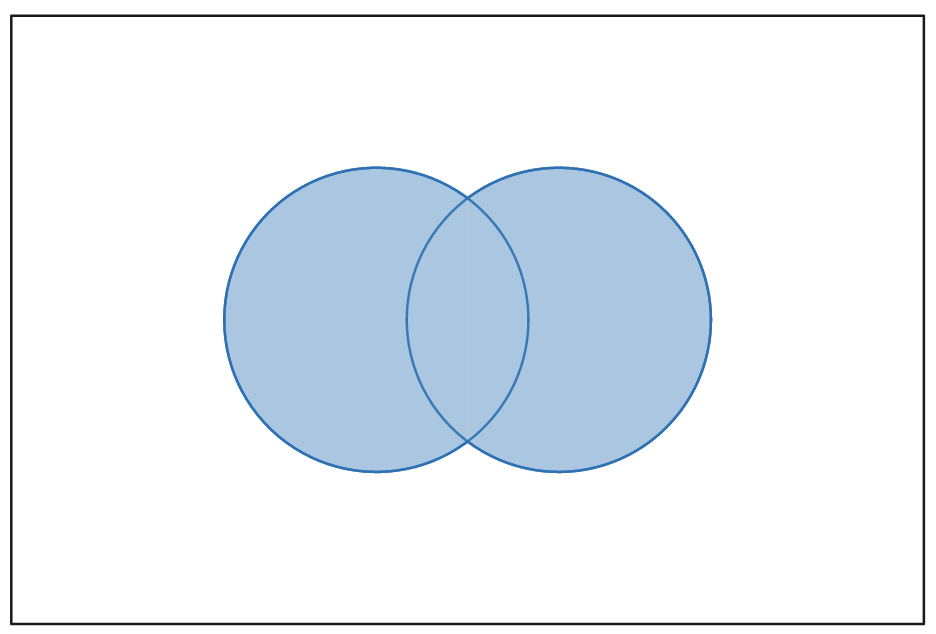
\includegraphics[scale=0.20]{union.png}};
         \draw (-3.5, 1.8)node{$U$};
         \draw (-1.5, 1)node{$A$};
         \draw (1.5, 1)node{$B$};
         \end{tikzpicture}\vspace{-8pt}
         \caption{Union}
     \end{subfigure}
     \begin{subfigure}[b]{0.425\textwidth}
        \centering
         \begin{tikzpicture}
         \node (union) at (0, 0){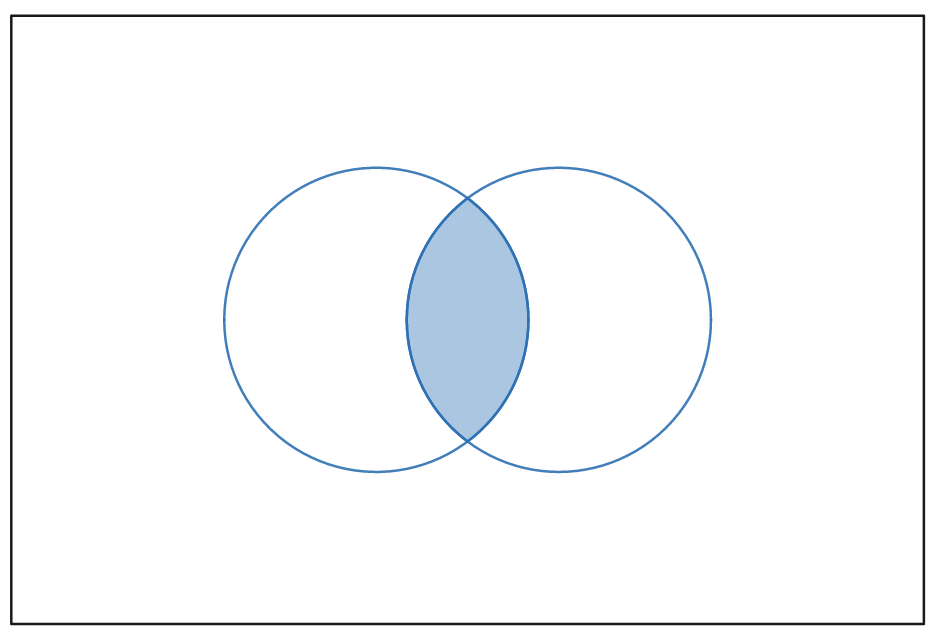
\includegraphics[scale=0.20]{intersection.png}};
         \draw (-3.5, 1.8)node{$U$};
         \draw (-1.5, 1)node{$A$};
         \draw (1.5, 1)node{$B$};
         \end{tikzpicture}\vspace{-8pt}
         \caption{Intersection}
     \end{subfigure}
    %\caption{Illustration of Union and Intersection Operations}
\end{figure}

\newpage


\underline{\textbf{Notes:}}
    \begin{itemize}
        \item Using the mathematical language from Appendix L, we can rewrite the union of $A$ and $B$ as followed: $A \cup B = \{ x \in U \, : \, x \in A \text{ or } x \in B\}$.
        \item Similarly, we can rewrite the intersection of $A$ and $B$ as followed: $A \cap B = \{ x \in U \, : \,  x \in A \text{ and } x \in B\}$.
    \end{itemize}

\begin{definition}
a) The \underline{complement} of a set is the new set $\overline{A}$ of all elements in $U$ that are not in $A$. Note that $A \cup \overline{A} = U$.\\
b) The \underline{set difference} of two sets $A$ and $B$ is the set $A \cap \overline{B}$. In other words, it is the set of elements that are in $A$, but not in $B$.
\end{definition}
    
    \begin{figure}[ht]
    \centering
     \begin{subfigure}[b]{0.45\textwidth}
        \centering
        \begin{tikzpicture}
         \node (union) at (0, 0){ 
\includegraphics[scale=0.22]{complement.png}};
         \draw (-3.8, 1.8)node{$U$};
         \draw (0, 0.75)node{$A$};
         \end{tikzpicture}\vspace{-8pt}
         \caption{Complement}
     \end{subfigure}
     \begin{subfigure}[b]{0.45\textwidth}
         \centering
          \begin{tikzpicture}
         \node (union) at (0, 0){ 
         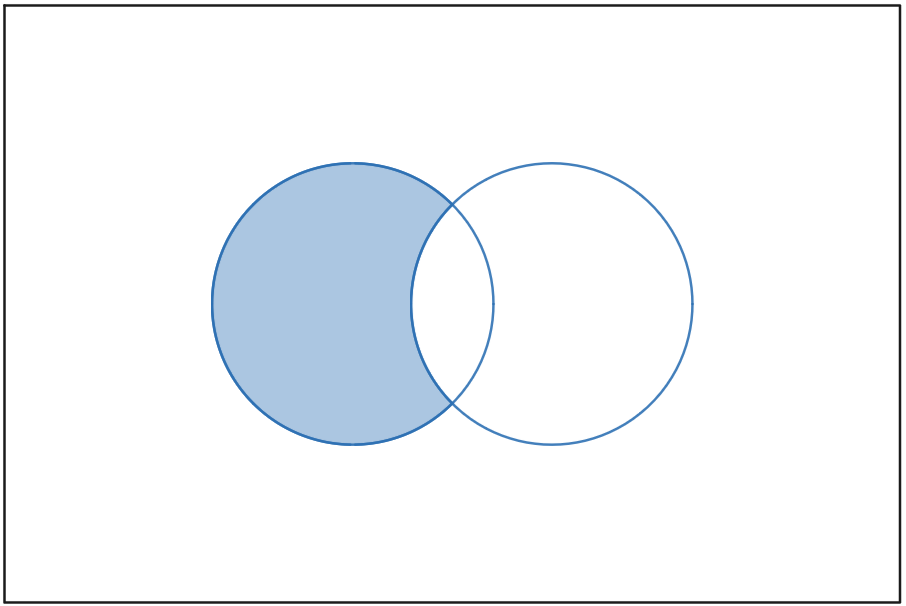
\includegraphics[scale=0.225]{difference.png}};
         \draw (-3.8, 1.8)node{$U$};
         \draw (-1.75, 1)node{$A$};
         \draw (1.75, 1)node{$B$};
         \end{tikzpicture}\vspace{-7pt}
         \caption{Difference}
     \end{subfigure}
    %\caption{Illustration of each operation}
    \end{figure}

    \underline{\textbf{Notes:}}
        \begin{itemize}
            \item We can rewrite the complement of a set $A$ as followed: $\overline{A} = \{ x \in U \, : \, x \not \in A \}$.
            \item We can rewrite the set difference of $A$ and $B$ as followed: $A \cap \overline{B} = \{ x \in U \, : \, x \in A \text{ and } x \not\in B \}$.
        \end{itemize}


    \begin{definition}
    Two sets, $A$ and $B$, are \underline{disjoint} or \underline{mutually exclusive} if $A \cap B = \varnothing$.
    \end{definition}

    \begin{example}
    Let $U= \{ 1 , 2, 3, 4 , 5 \}$. The sets $A = \{ 1 , 2 \}$ and $B = \{ 3 \}$ are mutually exclusive because they have nothing in common, meaning $A \cap B = \varnothing$.
    \end{example}

\newpage 

\section{Important Laws for Set Algebra}
    
    \begin{theorem}
        \begin{enumerate}[label=\alph*)]
        \item Commutative laws:
            \begin{align*}
            A \cup B = B \cup A \quad \text{and} \quad A \cap B = B \cap A .
            \end{align*}
        \item The distributive laws:
            \begin{align}
            A \cap (B \cup C ) &= (A \cap B) \cup (A \cap C ) \\
            A \cup (B \cap C ) &= (A \cup B) \cap (A \cup C ) .
            \end{align}
        \end{enumerate}
    \end{theorem}
    \begin{proof}
    We will prove one of the commutative laws and one of the distributive laws. The other formulas are left as an exercise.

    \begin{enumerate}[label=\alph*)]
    \item To prove the equation $A \cup B = B \cup A$, we have to show (i)$A \cup B \subset B \cup A$ and; (ii)$B \cup A \subset A \cup B$. 
        \begin{enumerate}[label=(\roman*)]
        \item Assume $x \in A \cup B$. Then, $x \in A$ or $x \in B$ by definition of the union of sets. But, this is the same thing as writing $x \in B$ or $x \in A$ (the order of the presentation is unimportant). Therefore, the element $x$ belongs to $B \cup A$ by definition of the union of $B$ and $A$. 
        \item Now, assume $x \in B \cup A$. Then $x \in B$ or $x \in A$ from the definition of $B \cup A$. Since the order of the presentation is unimportant, $x \in A$ or $x \in B$. Therefore, $x \in A \cup B$ by definition of the union of $A$ and $B$. 
        \end{enumerate}
        Let's wrap this up. We just proved that $A \cup B \subset B \cup A$ and that $B \cup A \subset A \cup B$. From the definition of equality of sets, this means $A \cup B = B \cup A$.
    \item We prove the equation $A \cap (B \cup C) = (A \cap B) \cup (A \cap C)$. 
        \begin{enumerate}[label=(\roman*)]
        \item We start by proving that $A \cap (B \cup C) \subset (A \cap B) \cup (A \cap C)$. Assume $x \in A \cap (B \cup C)$. Then, by definition of the intersection of two sets, this means $x \in A$ and $x \in B \cup C$. By definition of the union of two sets, $x \in B \cup C$ implies that $x \in B$ or $x \in C$. Since $x$ belongs to $A$ in both cases, then if $x$ belongs to $B$, we conclude that $x$ belongs to $A \cap B$, but if $x$ belongs to $C$, we conclude that $x$ belongs to $A \cap C$. Therefore, $x$ belongs to $A \cap B$ or to $A \cap C$. By definition of the union, the element $x$ belongs to $(A \cap B) \cup (A \cap C)$. 
        \item Now we prove that $(A \cap B) \cup (A \cap C) \subset A \cap (B \cup C)$. Assume $x \in (A \cap B) \cup (A \cap C)$. Then, this means that $x$ belongs to $A \cap B$ or to $A \cap C$. The fact $x \in A \cap B$ implies that $x \in A$ and $x \in B$. The second fact that $x \in A \cap C$ implies that $x \in A$ and $x \in C$. Since $x$ belongs to $A$ in both cases, we see that $x \in A$ and $x$ belongs to $B$ or to $C$. In other words, the element $x$ belongs to $A$ and to $B \cup C$, which means that $x \in A \cap (B \cup C)$.
        \end{enumerate}
        From (i) and (ii), we can then conclude that $A \cap (B \cup C) = (A \cap B) \cup (A \cap C)$.
    \end{enumerate}
    \end{proof}

    \begin{theorem}
    De Morgan's laws:
        \begin{align*}
        \overline{A \cap B} = \overline{A} \cup \overline{B} \quad \text{ and } \quad \overline{A \cup B} = \overline{A} \cap \overline{B} .
        \end{align*}
    \end{theorem}
    \begin{proof}
    We only prove the first equation and leave the proof of the second one as an exercise. 

    Suppose $x \in \overline{A \cap B}$. From the definition of the complement of a set, $x \not\in A \cap B$. this means that $x$ does not belong to $A \cap B$. We have to negate the definition of intersection. We have $x \in A \cap B$ when $x \in A$ \textit{and} $x \in B$. The negation is $x \not\in A$ or $x \not\in B$. Therefore, $x \in \overline{A}$ or $x \in \overline{B}$. From the definition of the union of two sets, we see that $x \in \overline{A} \cup \overline{B}$.

    Now, assume $x \in \overline{A} \cup \overline{B}$. This means that $x \not\in A$ or $x \not\in B$. From the last paragraph, this last statement is the negation of $x \in A \cap B$. Therefore, $x \not\in A \cap B$. In other words, $x$ belongs to $\overline{A \cap B}$. 

    We can then conclude that $\overline{A \cap B} = \overline{A} \cup \overline{B}$. 
    \end{proof}

\begin{comment}
\section{Problems Set}

\subsection*{Terminology}

\begin{problem}
Let $U = \{1 , 2, 3, 4, 5 \}$, $A = \{ 1 , 2 \}$, and $B = \{ 1 , 2, 3\}$. Show that $A \subset B$.
\end{problem}

\begin{problem}
Let $U = \{ 1 , 2, 3, 4\}$. Show that $U$ has $2^4$ subsets. \underline{Bonus:} In general, show that if $U$ has a finite number of elements, then $U$ has $2^{(\#U)}$ subsets.
\end{problem}

\begin{problem}
Show that if $A$ is a set, then $\varnothing \subset A$.
\end{problem}

\begin{problem}
Let $A$, $B$, and $C$ be subsets of a universal set $U$. Show that if $A \subset B$ and $B \subset C$, then $A \subset C$.
\end{problem}

\subsection*{Operations With Sets}

\begin{problem}
Let $A$ and $B$ be two subsets of a universal set $U$.
    \begin{enumerate}[label=\alph*)]
        \item Show that $A \cap B \subset A$.
        \item Show that $A \subset A \cup B$.
        \item Show that if $A \subset B$, then $A \cup B = B$.
        \item Show that if $A \subset B$, then $A \cap B = A$.
    \end{enumerate}
\end{problem}

\begin{problem}
Let $A$ and $B$ be two subsets of a universal set $U$.
    \begin{enumerate}[label=\alph*)]
        \item Show that $A \cup \overline{A} = U$.
        \item Show that if $A \subset B$, then $\overline{B} \subset \overline{A}$.
    \end{enumerate}
\end{problem}

\begin{problem}
Let $A = \{ n \, : \, n \text{ is an odd integer}\}$ and let $B = \{ n \, : \, n \text{ is an even integer}\}$. Show that $A \cap B = \varnothing$. \textit{[Hint: To prove $A \cap B \subset \varnothing$, use the method of proof by contradiction.]}
\end{problem}

\subsection*{Important Laws For Set Algebra}

\begin{problem}
Let $A$, $B$, and $C$ be subsets of a universal set $U$.
    \begin{enumerate}[label=\alph*)]
        \item Prove that $A \cap B = B \cap A$.
        \item Prove that $A \cup (B \cap C) = (A \cup B) \cap (A \cup C)$.
        \item $\overline{A \cup B} = \overline{A} \cap \overline{B}$.
    \end{enumerate}
\end{problem}




\section{Solutions to Problems Set}
\setcounter{problem}{0} 

\subsection*{Terminology}

\begin{problem}
Let $x \in A$. Then either $x = 1$ or $x = 2$. When $x = 1$, we see that $1 \in B$, so $x \in B$. When $x = 2$, we see that $2 \in B$, so that $x \in B$. Therefore, $\forall x \in A$, $x \in B$ and $A \subset B$.
\end{problem}

\begin{problem}
The power set of $U$ is 
\begin{align*}
2^U &= \{ \varnothing , \{ 1 \} , \{ 2 \} , \{ 3 \} , \{4 \} , \{ 1 , 2\} , \{ 1 , 3\} , \{ 1 , 4 \} , \{ 2 , 3\} , \{ 2, 4\} , \{ 3 , 4 \} , \\
& \phantom{=} \, \, \, \,  \{ 1 , 2, 3 \} , \{ 1 , 2, 4 \} , \{ 1 , 3 , 4, \} , \{ 2 , 3, 4, \} , U \} .
\end{align*}
Counting the number of subsets in the power set will give the total number of subsets of $U$. There are 16 items in the power set $2^U$ and $16 = 2^4$.

In general, define a subset $A$ of $U$ as a function $f_A : U \ra \{ 0 , 1\}$ in the following way:
    \begin{align*}
    f_A (x) = \left\{ \begin{matrix}
    1 & x \in A \\
    0 & x \not\in A .\end{matrix} \right. 
    \end{align*} 
Then the number of subsets of $U$ will be determined by the number of functions from $U$ into $\{ 0 , 1\}$. There are $2^{\#U}$ such functions because for each element $x \in U$, you have two possible choice for $f_A (x)$.
\end{problem}

\begin{problem}
By definition of $\varnothing \subset A$, we have to show that if $x \in \varnothing$, then $x \in A$. However, the assumption is always false and therefore the implication $x \in \varnothing \Rightarrow x \in A$ is always true. Thus $\varnothing \subset A$.
\end{problem}

\begin{problem}
Let $x \in A$. Since $A \subset B$, then $x \in B$. Now, since $B \subset C$, then $x \in C$. The element $x$ was arbitrarily chosen, so $A \subset C$.
\end{problem}

\subsection*{Operations With Sets}

\begin{problem}
Let $A$ and $B$ be two subsets of a universal set $U$.
    \begin{enumerate}[label=\alph*)]
        \item Let $x \in A \cap B$. By definition of intersection, we then have $x \in A$ and $x \in B$. In particular, we have $x \in A$. Since $x$ was arbitrary, then $A \cap B \subset A$.
        \item Let $x \in A$. Then the disjunction statement ``$x \in A$ or $x \in B$'' is true because $x \in A$ is assume to be true. Therefore, $x \in A \cup B$ by definition of the union of two sets. Since $x$ was arbitrary, then $A \subset A \cup B$.
        \item Assume that $A \subset B$. 
        We start by showing that $A \cup B \subset B$. If $x \in A \cup B$, then $x \in A$ or $x \in B$ by definition of union. Two cases:
            \begin{itemize}
            \item If $x \in A$, then $x \in B$ because $A \subset B$.
            \item If $x \in B$, then $x \in B$ (tautology).
            \end{itemize}
        In both cases, we obtain that $x \in B$. Since $x$ was arbitrary, we have $A \cup B \subset B$. We now show that $B \subset A \cup B$. From part b), we have $B \subset B \cup A$. Since $B \cup A = A \cup B$, we obtain $B \subset A \cup B$.

        Since $A \cup B \subset B$ and $B \subset A \cup B$, we have $A \cup B = B$.
        \item Assume that $A \subset B$. Let $x \in A \cap B$. Then $x \in A$ and $x \in B$. In particular $x \in A$. So $A \cap B \subset A$. Let $x \in A$. Then $x \in B$ also because $A \subset B$. Therefore $x \in A$ and $x \in B$ and so $x \in A \cap B$. So $A \subset A \cap B$. Since $A \cap B \subset A$ and $A \subset A \cap B$, we get $A \cap B = A$.
    \end{enumerate}
\end{problem}

\begin{problem}
Let $A$ and $B$ be two subsets of a universal set $U$.
    \begin{enumerate}[label=\alph*)]
        \item We have to show that $A \cup \overline{A} \subset U$ and $U \subset A \cup \overline{A}$. 

        Let $x \in A \cup \overline{A}$. There are two cases because of the definition of union:
            \begin{itemize}
                \item If $x \in A$, then $x \in U$ because $A \subset U$.
                \item If $x \in \overline{A}$, then $x \in U$ because $\overline{A} \subset U$.
            \end{itemize}
        Each case implies that $x \in U$. Therefore, $A \cup \overline{A} \subset U$.

        Let $x \in U$. Then $x \in A$ or $x \not\in A$ which implies that $x \in A \cup \overline{A}$. Therefore $U \subset A \cup \overline{A}$. 
        \item Assume that $A \subset B$. Let $x \in \overline{B}$. We will argue by contradiction. Suppose that $x \in A$. By assumption, this implies that $x \in B$. But $x \in \overline{B}$. In other words, $x \in B$ and $x \not\in B$. This is not possible and therefore $x \in \overline{A}$. [\textit{Note: You can also take the contrapositive for a direct proof! The contrapositive of $A \subset B$ is $x \not\in B \Rightarrow x \not\in A$ which is equivalent to $x \in \overline{B} \Rightarrow x \in \overline{A}$.}]
    \end{enumerate}
\end{problem}

\begin{problem}
Since $\varnothing \subset A \cap B$, we only need to prove that $A \cap B \subset \varnothing$. We will argue by contradiction. For $A \cap B$ to not be a subset of $\varnothing$, it must contain at least one element. So, assume that $x \in A \cap B$. This implies that $x \in A$ and $x \in B$. By definition of $A$, $x$ is an odd integer. By definition of $B$, $x$ is also an even integer. But an integer can't be odd and even at the same time by Example \ref{Ex:NoIntIsOddAndEven} and this is a contradiction. Therefore, $A \cap B \subset \varnothing$.

Since $\varnothing \subset A \cap B$ and $A \cap B \subset \varnothing$, we conclude that $A \cap B = \varnothing$.
\end{problem}

\subsection*{Important Laws For Set Algebra}

\begin{problem}
Let $A$, $B$, and $C$ be subsets of a universal set $U$.
    \begin{enumerate}[label=\alph*)]
        \item We have
            \begin{align*}
            x \in A \cap B & \iff x \in A \text{ and } x \in B \quad \text{[Definition of $A \cap B$]}\\
            & \iff x \in B \text{ and } x \in A \quad \text{[Order of words don't matter]} \\
            & \iff x \in B \cap A \quad \text{[Definition of $B \cap A$]}
            \end{align*}
        \item We start by showing that $A \cup (B \cap C) \subset (A \cup B) \cap (A \cup C)$. Let $x \in A \cup (B \cap C)$. Then by definition of the union, we have $x \in A$ or $x \in B \cap C$. The fact $x \in B \cap C$ implies that $x \in B$ and $x \in C$. In particular, $x \in B$. Combined with $x \in A$, we obtain $x \in A$ or $x \in B$. Similarly, we obtain $x \in A$ or $x \in C$. We can then create the conjunction of ``$x \in A$ or $x \in B$'' with ``$x \in A$ or $x \in C$'', that is $(x \in A \vee x \in B) \wedge (x \in A \vee x \in C)$. Using the definition of union, the last statement is rewritten as $(x \in A \cup B) \wedge (x \in A \cup C)$. From the definition of intersection, we can rewrite the last statement as $x \in (A \cup B) \cap (A \cup C)$. 

        To show that $(A \cup B) \cap (A \cup C) \subset A \cup (B \cap C)$ is similar. We just start from the end of the previous paragraph and make our way back to the first sentence of the paragraph (so read the last paragraph from the last sentence to the first sentence to obtain the proof). 

        Therefore, we just proved equality between the two sets.
        \item We have
            \begin{align*}
             x \in \overline{A \cup B} & \iff x \not\in A \cup B \\
             & \iff x \not\in A \wedge x \not\in B \quad \text{[Negation of $A \cup B$]} \\
             & \iff x \in \overline{A} \wedge x \in \overline{B} \quad \text{[Definition of complement]} \\
             & \iff x \in \overline{A} \cap \overline{B} \quad \text{[Definition of intersection]}.
             \end{align*}
        Therefore, $\overline{A \cup B} = \overline{A} \cap \overline{B}$.
    \end{enumerate}
\end{problem}

\end{comment}

\end{document}